\documentclass[11pt,twoside,a4paper]{book}  
% definice dokumentu
\usepackage[czech, english]{babel}
\usepackage[T1]{fontenc} 				% pouzije EC fonty 
\usepackage[utf8]{inputenc} 			% utf8 kódování vstupu 
\usepackage[square, numbers]{natbib}	% sazba pouzite literatury
\usepackage{indentfirst} 				% 1. odstavec jako v cestine, pro práci v aj možno zakomentovat
\usepackage{fancyhdr}					% tisk hlaviček a patiček stránek
\usepackage{nomencl}					% umožňuje snadno definovat zkratky a jejich seznam 
\usepackage{amsmath,amssymb,verbatim}

%%%%%%%%%%%%%%%%%%%%%%%%%%%%%%%%%%%%%%%%%%%%%%%%%%%%%%%%%%%%%%%
% informace o práci
\newcommand\WorkTitle{Editor hranic ploch pro program ArchiRec3D}		% název
\newcommand\FirstandFamilyName{Petr Beránek}															% autor
\newcommand\Supervisor{Ing. David Sedláček, Ph.D. }															% vedoucí

\newcommand\TypeOfWork{Bakalářská práce}	% typ práce [Diplomová práce | Bakalářská práce | Bachelor's Project | Master's Thesis ]	

% Nastavte následují podle vašeho oboru a programu (pomoc hledejte na http://www.fel.cvut.cz/cz/education/bk/prehled.html)								
\newcommand\StudProgram{Otevřená informatika, Bakalářský}	% program
\newcommand\StudBranch{Softwarové systémy}           					% obor

%%%%%%%%%%%%%%%%%%%%%%%%%%%%%%%%%%%%%%%%%%%%%%%%%%%%%%%%%%%%%%%
% minimální importy
\usepackage{graphicx}					% pro vkládání obrázků
\usepackage{k336_thesis_macros} 		% specialni makra pro formatovani DP a BP
\usepackage[
pdftitle={\WorkTitle},				% nastaví v informacích o pdf název
pdfauthor={\FirstandFamilyName},	% nastaví v informacích o pdf autora
colorlinks=true,					% před tiskem doporučujeme nastavit na false, aby odkazy a url nebyly šedé při ČB tisku
breaklinks=true,
urlcolor=red,
citecolor=blue,
linkcolor=blue,
unicode=true,
]
{hyperref}								% pro zobrazování "prokliknutelných" linků 

% rozšiřující importy
\usepackage{listings} 			%slouží pro tisk zdrojových kódů se syntax higlighting
\usepackage{algorithmicx} 		%slouží pro zápis algoritmů
\usepackage{algpseudocode} 		%slouží pro výpis pseudokódu

%%%%%%%%%%%%%%%%%%%%%%%%%%%%%%%%%%%%%%%%%%%%%%%%%%%%%%%%%%%%%%%
% příkazy šablony
\makenomenclature								% při překladu zajistí vytvoření pracovního souboru se seznamem zkratek

\let\oldUrl\url									% url adresy budou zobrazeny: <url> 
\renewcommand\url[1]{<\texttt{\oldUrl{#1}}>}

%%%%%%%%%%%%%%%%%%%%%%%%%%%%%%%%%%%%%%%%%%%%%%%%%%%%%%%%%%%%%%%
% vaše vlastní příkazy
\newcommand*{\nomExpl}[2]{#2 (#1)\nomenclature{#1}{#2}} 	% usnadňuje zápis zkratek : Slova ke Zkrácení (SZ)
\newcommand*{\nom}[2]{#1\nomenclature{#1}{#2}} 			% usnadňuje zápis zkratek : SZ



%%%%%%%%%%%%%%%%%%%%%%%%%%%%%%%%%%%%%%%%%%%%%%%%%%%%%%%%%%%%%%%
% vlastní dokument
%%%%%%%%%%%%%%%%%%%%%%%%%%%%%%%%%%%%%%%%%%%%%%%%%%%%%%%%%%%%%%%
\begin{document}
	
	%%%%%%%%%%%%%%%%%%%%%%%%%% 
	% nastavení jazyka, kterým je práce psána
	\selectlanguage{czech}	% podle jazyka práce nastavte na [czech | english]
	\translate				% nastaví české nebo anglické popisy (např. katedra -> department); viz k336_thesis_macros

	%%%%%%%%%%%%%%%%%%%%%%%%%%    
	% Poznamky ke kompletaci prace
	% Nasledujici pasaz uzavrenou v {} ve sve praci samozrejme 
	% zakomentujte nebo odstrante. 
	% Ve vysledne svazane praci bude nahrazena skutecnym 
	% oficialnim zadanim vasi prace.
	{
	\pagenumbering{roman} \cleardoublepage \thispagestyle{empty}
	\chapter*{Na tomto místě bude oficiální zadání vaší práce}
	\begin{itemize}
		\item Toto zadání je podepsané děkanem a vedoucím katedry,
		\item musíte si ho vyzvednout na studijním oddělení Katedry počítačů na Karlově náměstí,
		\item v jedné odevzdané práci bude originál tohoto zadání (originál zůstává po obhajobě na katedře),
		\item ve druhé bude na stejném místě neověřená kopie tohoto dokumentu (tato se vám vrátí po obhajobě).
	\end{itemize}
	\newpage
	}

	%%%%%%%%%%%%%%%%%%%%%%%%%%    
	% Titulni stranka / Title page 
	\coverpagestarts

	%%%%%%%%%%%%%%%%%%%%%%%%%%%    
	% Poděkovani / Acknowledgements 

	\acknowledgements
	\noindent
	Zde bych chtěl poděkovat vedoucímu práce, Ing. Davidu Sedláčkovi, Ph.D., za konzultace a za cenné rady. Dále bych chtěl poděkovat své rodině za podporu během celého mého studia a především v době psaní této práce. Zároveň bych rád poděkoval všem lidem, kteří se zúčastnili testování aplikace, čímž mi poskytli cennou zpětnou vazbu.


	%%%%%%%%%%%%%%%%%%%%%%%%%%%   
	% Prohlášení / Declaration 

	\declaration{V~Kladně dne 18.\,5.\,2015}
	%%%%%%%%%%%%%%%%%%%%%%%%%%%%    
	% Abstrakt / Abstract 
 
	\abstractpage
	\noindent
	The goal of this thesis is to analyze 3D reconstruction application ArchiRec3D and to design and implement several tools, which give user new possibilities of plane editing. 
	One of the tools allows user to create/modify borders, which are used to trim the planes. Other tool allows user to apply texture to these trimmed planes. The next important tool allows user to create 3D objects form trimmed plane. 
	Thesis contains analysis of the most important parts of the application. There are also chapters containing problem analysis, design, implementation and testing of these tools.
	The result is the modified application which allows user to create more detailed textured objects, which was not possible before.
	\paragraph{}
	\noindent
	\textbf{Keywords: }ArchiRec3D, user assisted 3D reconstruction, texture extraction, structure from motion, computer vision, computer graphics
	
	\vglue40mm

	\noindent{\Huge \textbf{Abstrakt}}
	\vskip 2.75\baselineskip

	\noindent
	Cílem mé práce bylo analyzovat program pro 3D rekonstrukci ArchiRec3D a implementovat nástroje pro zadávání, modifikaci a aplikaci hranice na rekonstruované plochy. Dále vytvoření nástrojů pro texturování těchto upravených ploch a vytváření 3D těles na jejich základě.
	Práce kromě analýzy stávajícího stavu programu obsahuje především části týkající se vytvářených nástrojů. Konkrétně analýzu problému, návrh řešení a popis implementace těchto nástrojů.
	Výsledkem této práce je modifikovaný program, který nyní obsahuje výše zmíněné nástroje, čímž umožňuje uživateli vytvářet detailní texturované objekty, což dříve v tomto programu nebylo možné.
	\paragraph{}
	\noindent
	\textbf{Klíčová slova: }ArchiRec3D, uživatelem řízená 3D rekonstrukce, extrakce textur, rekonstrukce z fotografií, počítačové vidění, počítačová grafika
	
	%%%%%%%%%%%%%%%%%%%%%%%%%%    
	% obsahy a seznamy
	\tableofcontents		% Obsah / Table of Contents 

	% pokud v práci nejsou obrázky nebo tabulky - odstraňte jejich seznam
	\listoffigures			% Obsah / Table of Contents 
	%\listoftables			% Seznam tabulek / List of Tables

	%%%%%%%%%%%%%%%%%%%%%%%%%% 
	% začátek textu  
	\mainbodystarts

\chapter{Úvod}
\paragraph{}
V celé své práci se budu převážně zabývat experimentálním programem ArchiRec3D\cite{ViCiTiS}, jenž slouží k vytváření 3D rekonstrukcí budov. Uživatel v tomto programu pracuje se scénou (\ref{scena}) a může v ní vytvářet plochy, díky čemuž je schopen v krátkém čase vytvořit hrubý model reprezentující rekonstruovaný objekt. Důraz je zde především kladen na to, aby uživatel nemusel zadávat veliké množství dat, a také aby tato data nemusela být naprosto přesná.
\paragraph{}
Uživatel sice může vytvářet objekty v poměrně krátkém čase, ale aktuální implementace nabízí pouze malé množství nástrojů, kterými může uživatel do scény zasahovat. Zároveň plochy, které uživatel vytváří, mají velmi omezené tvary. (plocha má obdélníkový tvar a dvě plochy se mohou navzájem ořezávat v místě jejich průsečíku.) Vytvoření nekonvexních polygonů z ploch ořezáváním není možné a vytváření složitějších konvexních polygonů je poměrně náročné. K tomu všemu je každá plocha obarvena jednou barvou, která jí byla určena.

\section{Cíl práce}
\label{cil}  
Mým cílem v této práci bude analyzovat implementaci tohoto programu a na základě této analýzy následně navrhnout a implementovat sadu nástrojů. V této sadě budou především nástroje pro zadání, upravení a aplikaci hranice, která bude ořezávat příslušnou plochu. Tím bude uživatel schopen vytvářet plochy libovolně složitých tvarů. Další nástroj bude pro texturování takto oříznutých ploch pomocí vybrané fotografie.  A nakonec nástroj, který uživateli dovolí z oříznuté plochy vytvořit trojrozměrné těleso.
\paragraph{}
Jak bylo výše zmíněno, program používá data scény, kterou je nezbytné před počátkem práce importovat. Tuto scénu je možné získat například programem Bundler \cite{Snavely}. Obdobný typ scény je vytvářen i programem VisualSFM \cite{SFM} \cite{MBA}, ale má lehce odlišný formát. Naproti tomu je program VisualSFM poměrně snadný na používání. Proto kromě předchozích nástrojů budu ještě vytvářet importní modul pro data z tohoto programu.

%
%
%
\chapter{Analýza}
V této části se budu zabývat analýzou stavu programu ArchiRec3D a jeho základní architekturou. Dále zde bude analýza jednotlivých problémů, které se při modifikaci programu vyskytují. Na analýzu těchto problémů bude následně navazovat návrh jejich řešení.

\section{Popis programu ArchiRec3D}
Nyní zde popíši základní strukturu programu. Tato část obsahuje pouze vybranou část programu, která se vztahuje k jeho základním funkcím a k problémům, které bude nutné vyřešit(viz. \ref{cil}). 

\subsection{ArchiRec3D}
Jak již bylo zmíněno v úvodu, ArchiRec3D je experimentální program pro 3D rekonstrukci budov. Celý program je psán v jazyce Java a pro vizualizaci využívá knihovnu Java 3D. Pro rekonstruování objektu je kromě vstupů od uživatele nezbytné před začátkem práce importovat scénu(\ref{scena}). 

\subsection{Scéna}
\label{scena}
Scéna je objekt, který obaluje množinu fotografií, kamer(\ref{kamera}) a mračna bodů(\ref{mracno}). Jak již bylo zmíněno dříve, takovouto scénu je možné získat například pomocí programů jako Bundler nebo VisualSFM. Scéna získaná těmito programy využívá formát "Bundle file v0.3" \cite{BundleMan}.

\subsection{Kamera}
\label{kamera}
Scéna je vytvářena z fotografií a během jejího vytváření jsou odhadnuty pozice, ze které byly fotografie pořízeny, a také směr, kterým byla fotografie focena. Tyto parametry jsou spolu s dalšími parametry fotoaparátu uloženy do objektu kamery. To znamená, že kamera ve scéně reprezentuje místo, odkud ve scéně byla fotografie pořízena a dále uchovává parametry zařízení, které fotografii pořídilo. Kromě pozice a rotace kamera obsahuje také svou ohniskovou vzdálenost, dva radial distortion parametry a odkaz na svou fotografii. 

\subsection{Mračno bodů}
\label{mracno}
Mračno bodů je množina trojrozměrných bodů v prostoru. Každý z těchto bodů je reprezentován svou pozicí, barvou a také seznamem fotografií, ve kterých se tento bod vyskytuje. Zároveň je v tomto listu také pozice, kde se tento bod v dané fotografii vyskytuje. 

\begin{figure}[h]
	\begin{center}
		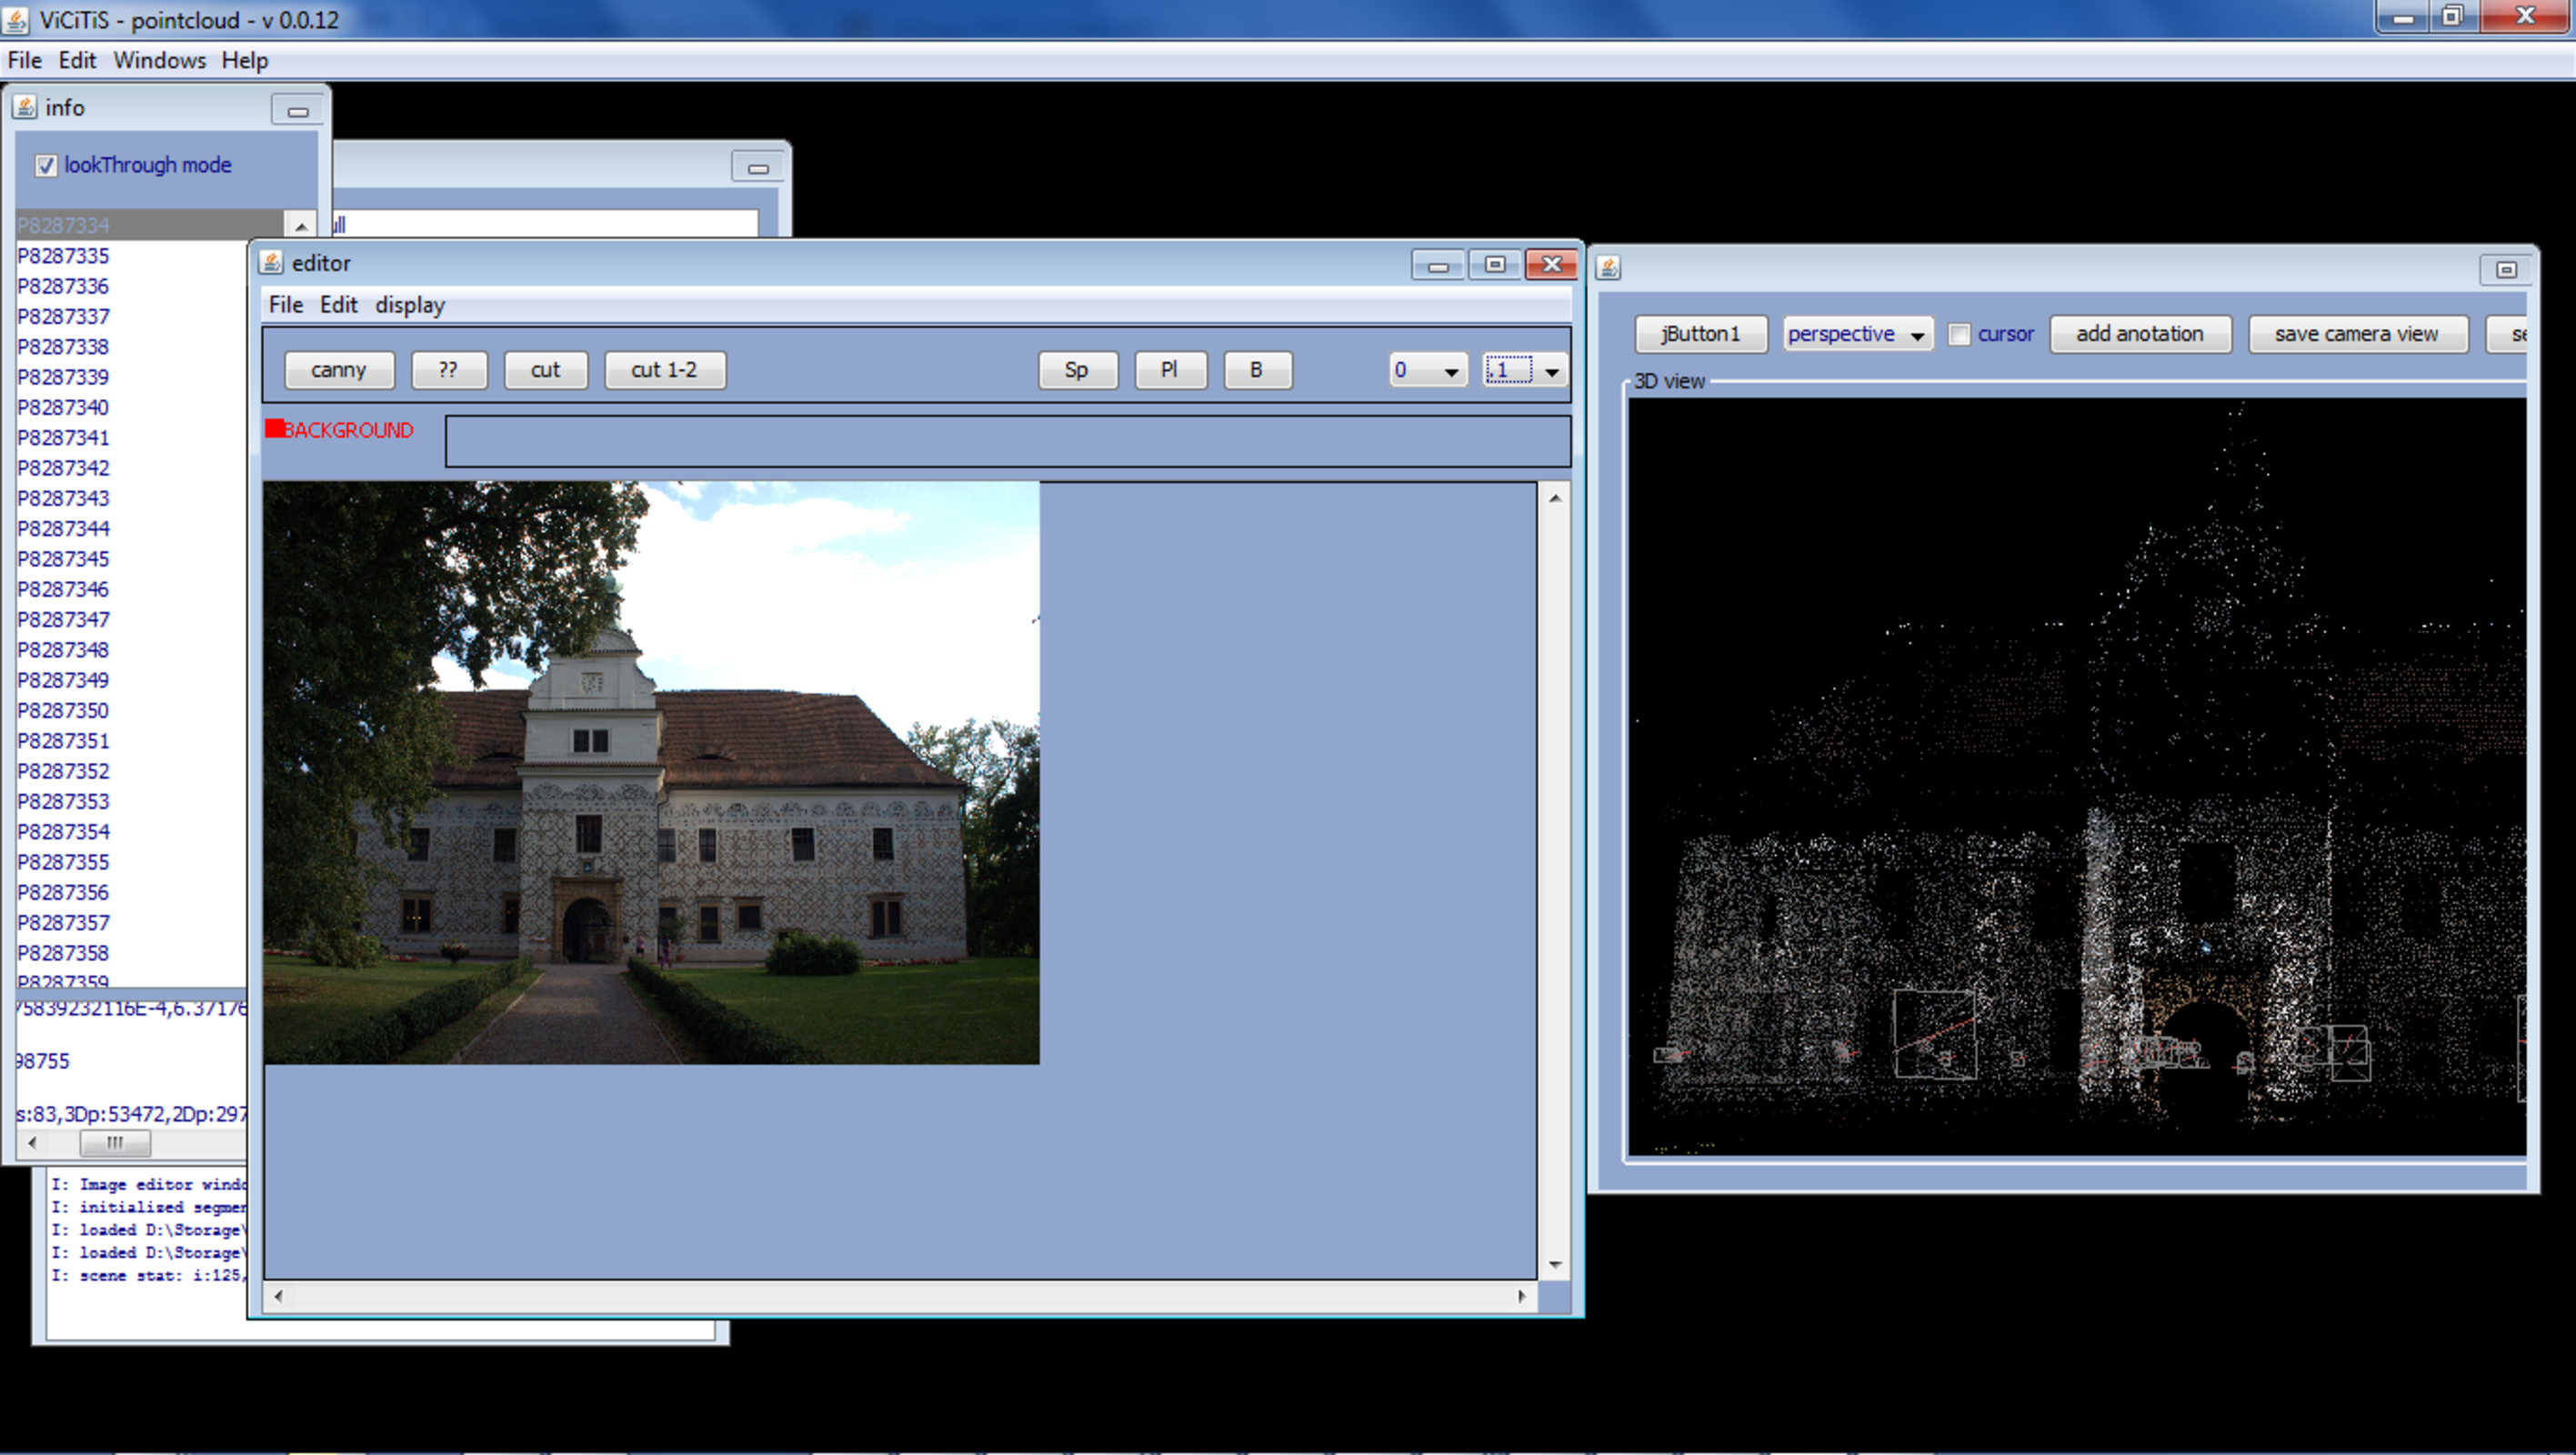
\includegraphics[width=15cm]{ilustrace/Il-1-1}
		\caption{Ilustrace znázorňující vzhled celé aplikace.}
		\label{fig:1-1}
	\end{center}
\end{figure}

\begin{figure}[]
	\begin{center}
		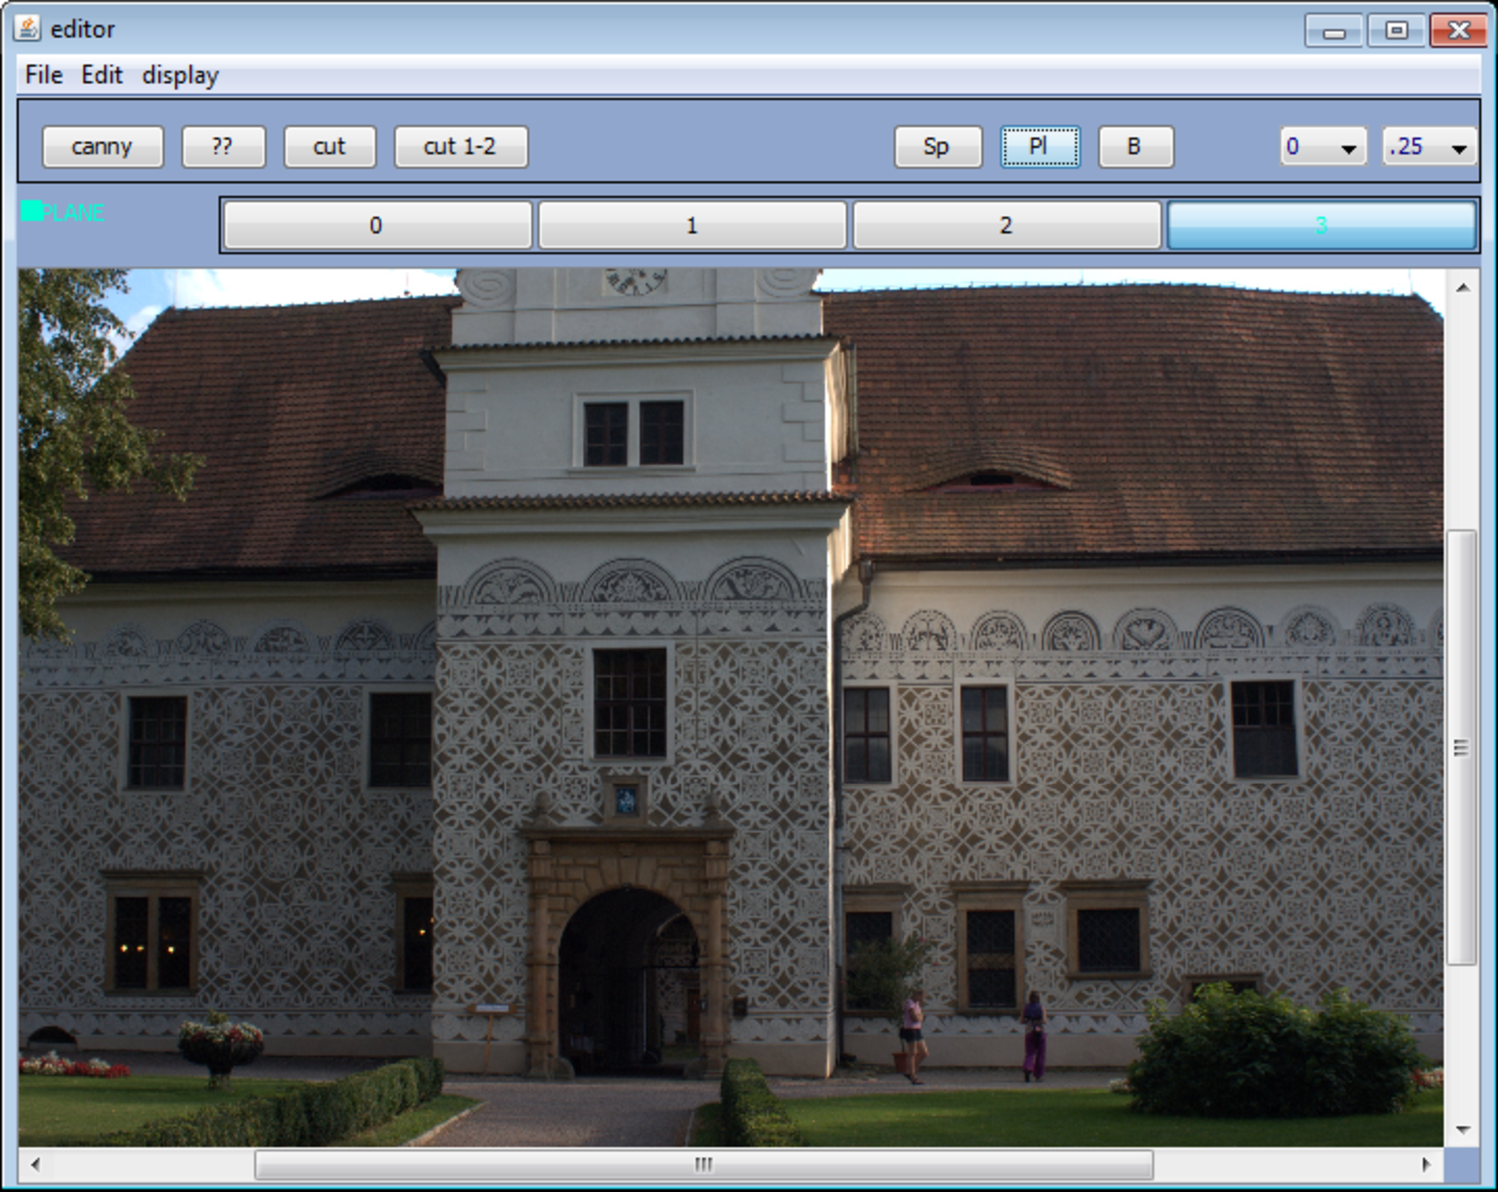
\includegraphics[width=14cm]{ilustrace/Il-1-2}
		\caption{Ilustrace znázorňující okno editoru fotografií.}
		\label{fig:1-2}
	\end{center}
\end{figure}

\begin{figure}[]
	\begin{center}
		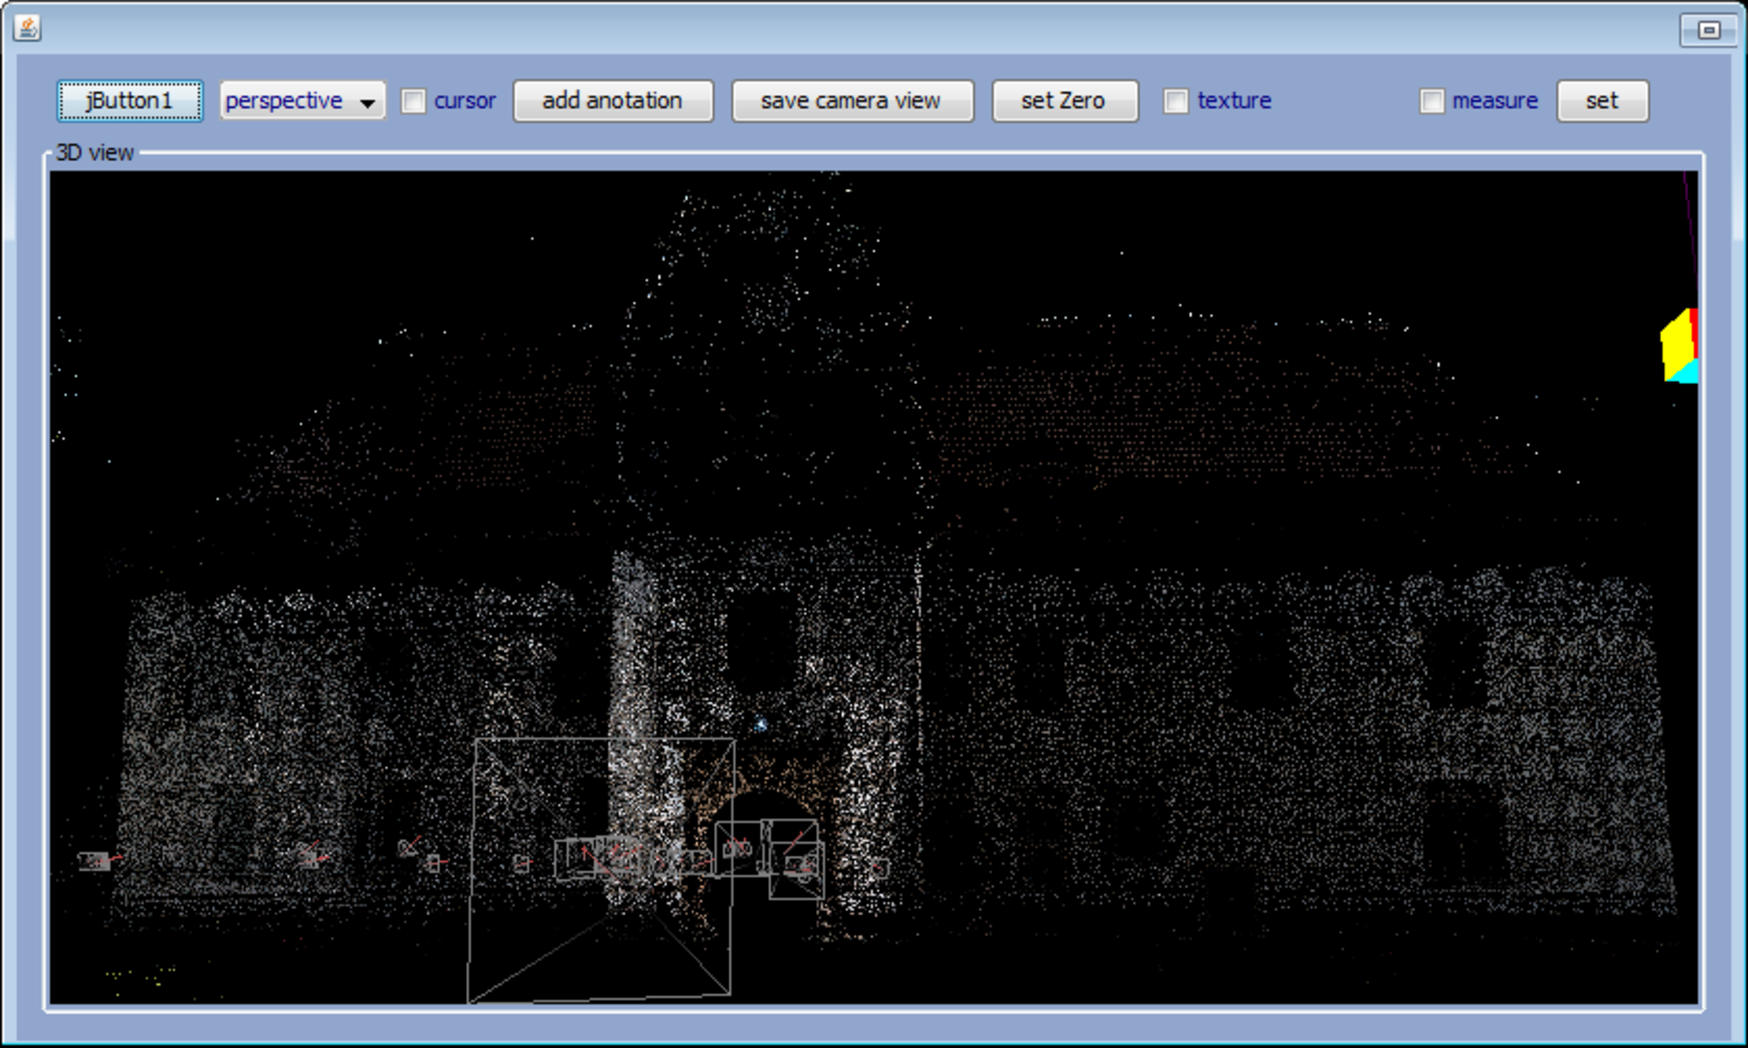
\includegraphics[width=13cm]{ilustrace/Il-1-3}
		\caption{Ilustrace znázorňující okno 3D scény.}
		\label{fig:1-3}
	\end{center}
\end{figure}

\begin{figure}[]
	\begin{center}
		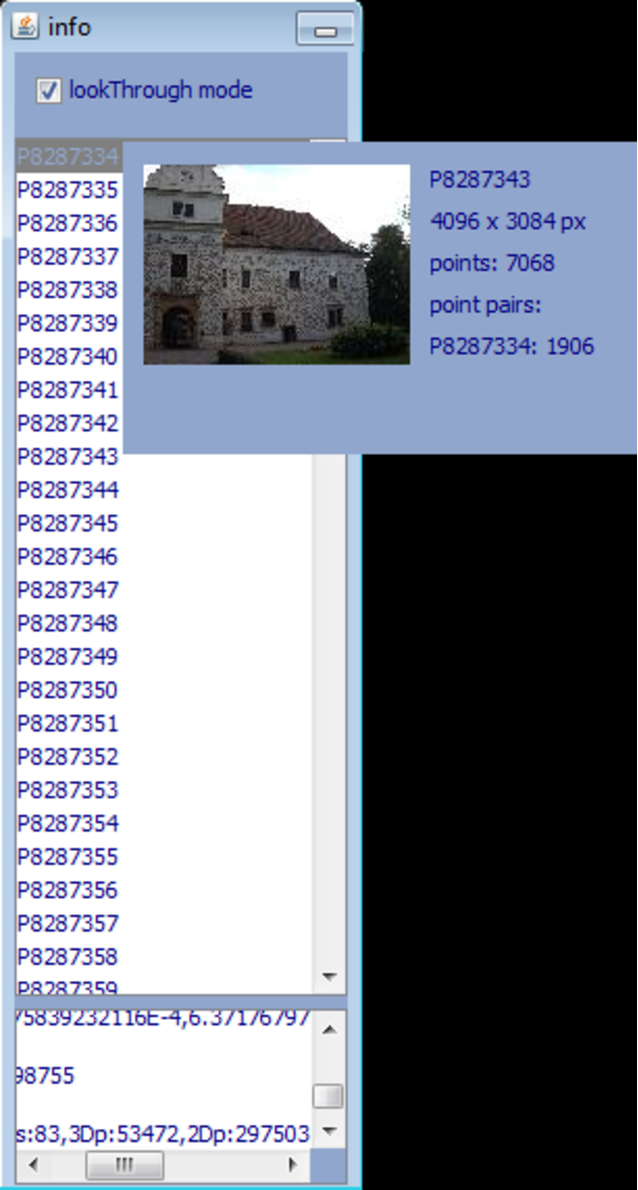
\includegraphics[width=6cm]{ilustrace/Il-1-4}
		\caption{Ilustrace znázorňující okno info panelu.}
		\label{fig:1-4}
	\end{center}
\end{figure}

\begin{figure}[]
	\begin{center}
		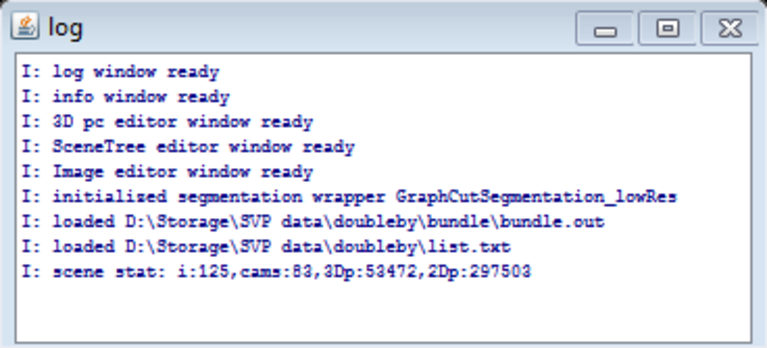
\includegraphics[width=10cm]{ilustrace/Il-1-5}
		\caption{Ilustrace znázorňující okno logu.}
		\label{fig:1-5}
	\end{center}
\end{figure}

\clearpage

\begin{figure}[t]
	\begin{center}
		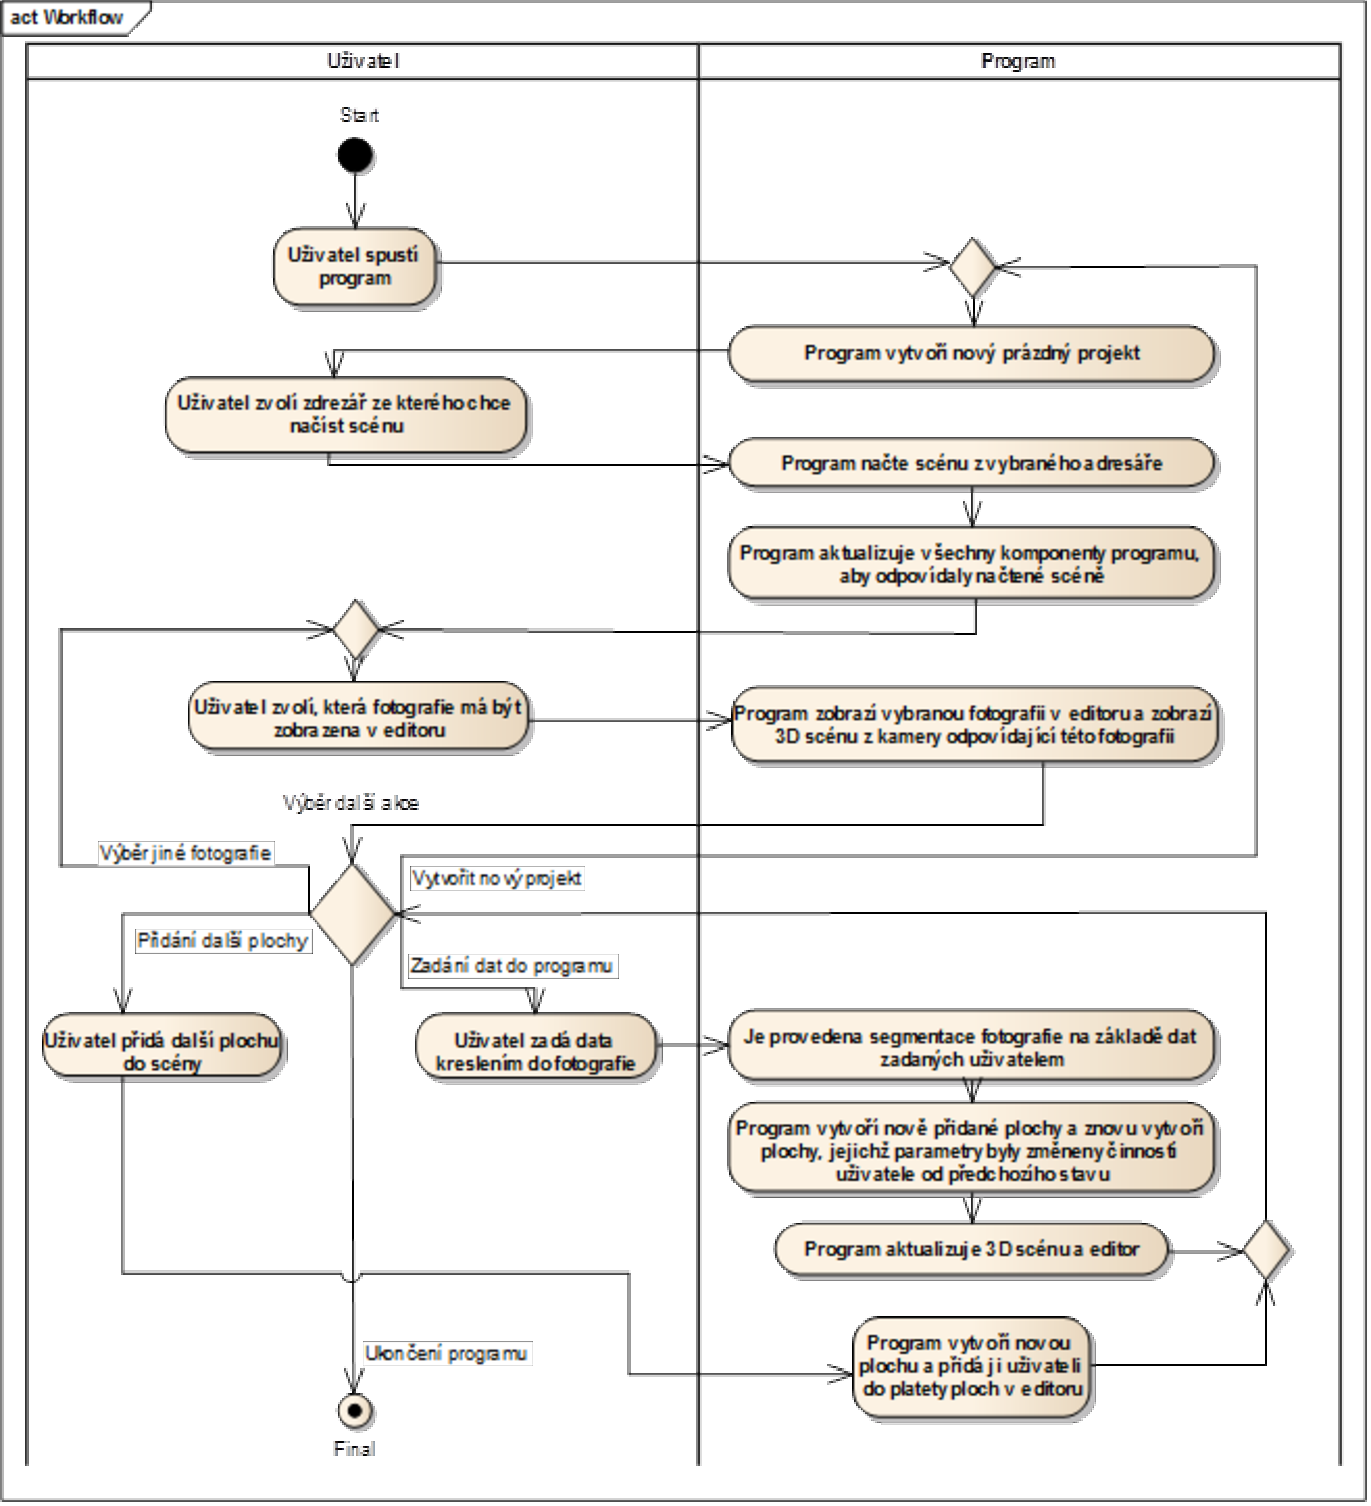
\includegraphics[width=14cm]{ilustrace/Workflow}
		\caption{Ilustrace znázorňující uživatelovy možnosti.}
		\label{fig:workflow}
	\end{center}
\end{figure}

\clearpage



\subsection{Možnosti uživatele}
Program se skládá především z editoru fotografie a 3D scény. Uživatel si může v editoru zobrazit libovolnou fotografii scény. Následně uživatel může přidat libovolné množství ploch.Pro zobrazení ploch ve 3D scéně je nezbytné, aby uživatel zadal pro danou plochu do fotografie data pro segmentaci fotografie. 
\paragraph{}
Tato data se zadávají kreslením pomocí kurzoru ve fotografii. K proběhnutí segmentace fotografie, uživatel musí zadat data alespoň pro dvě plochy v jedné fotografii. Když je zadáno dostatečné množství dat, je provedena segmentace fotografie. Tím získáme oblasti ve fotografii, které odpovídají jednotlivým plochám. Díky znalosti, kde se v dané fotografii nacházejí body získané při kalibraci scény, je možné určit, který bod odpovídá které ploše.
\paragraph{}
Tyto body program proloží rovinou a rovinu ořízne. Oříznuté roviny reprezentují plochy a jsou zobrazeny v 3D scéně. Uživatel také může nastavit, aby se některé plochy mezi sebou navzájem ořezávaly. To umožňuje vytvářet přesné rohy stěn a budov.

\begin{figure}[h]
	\begin{center}
		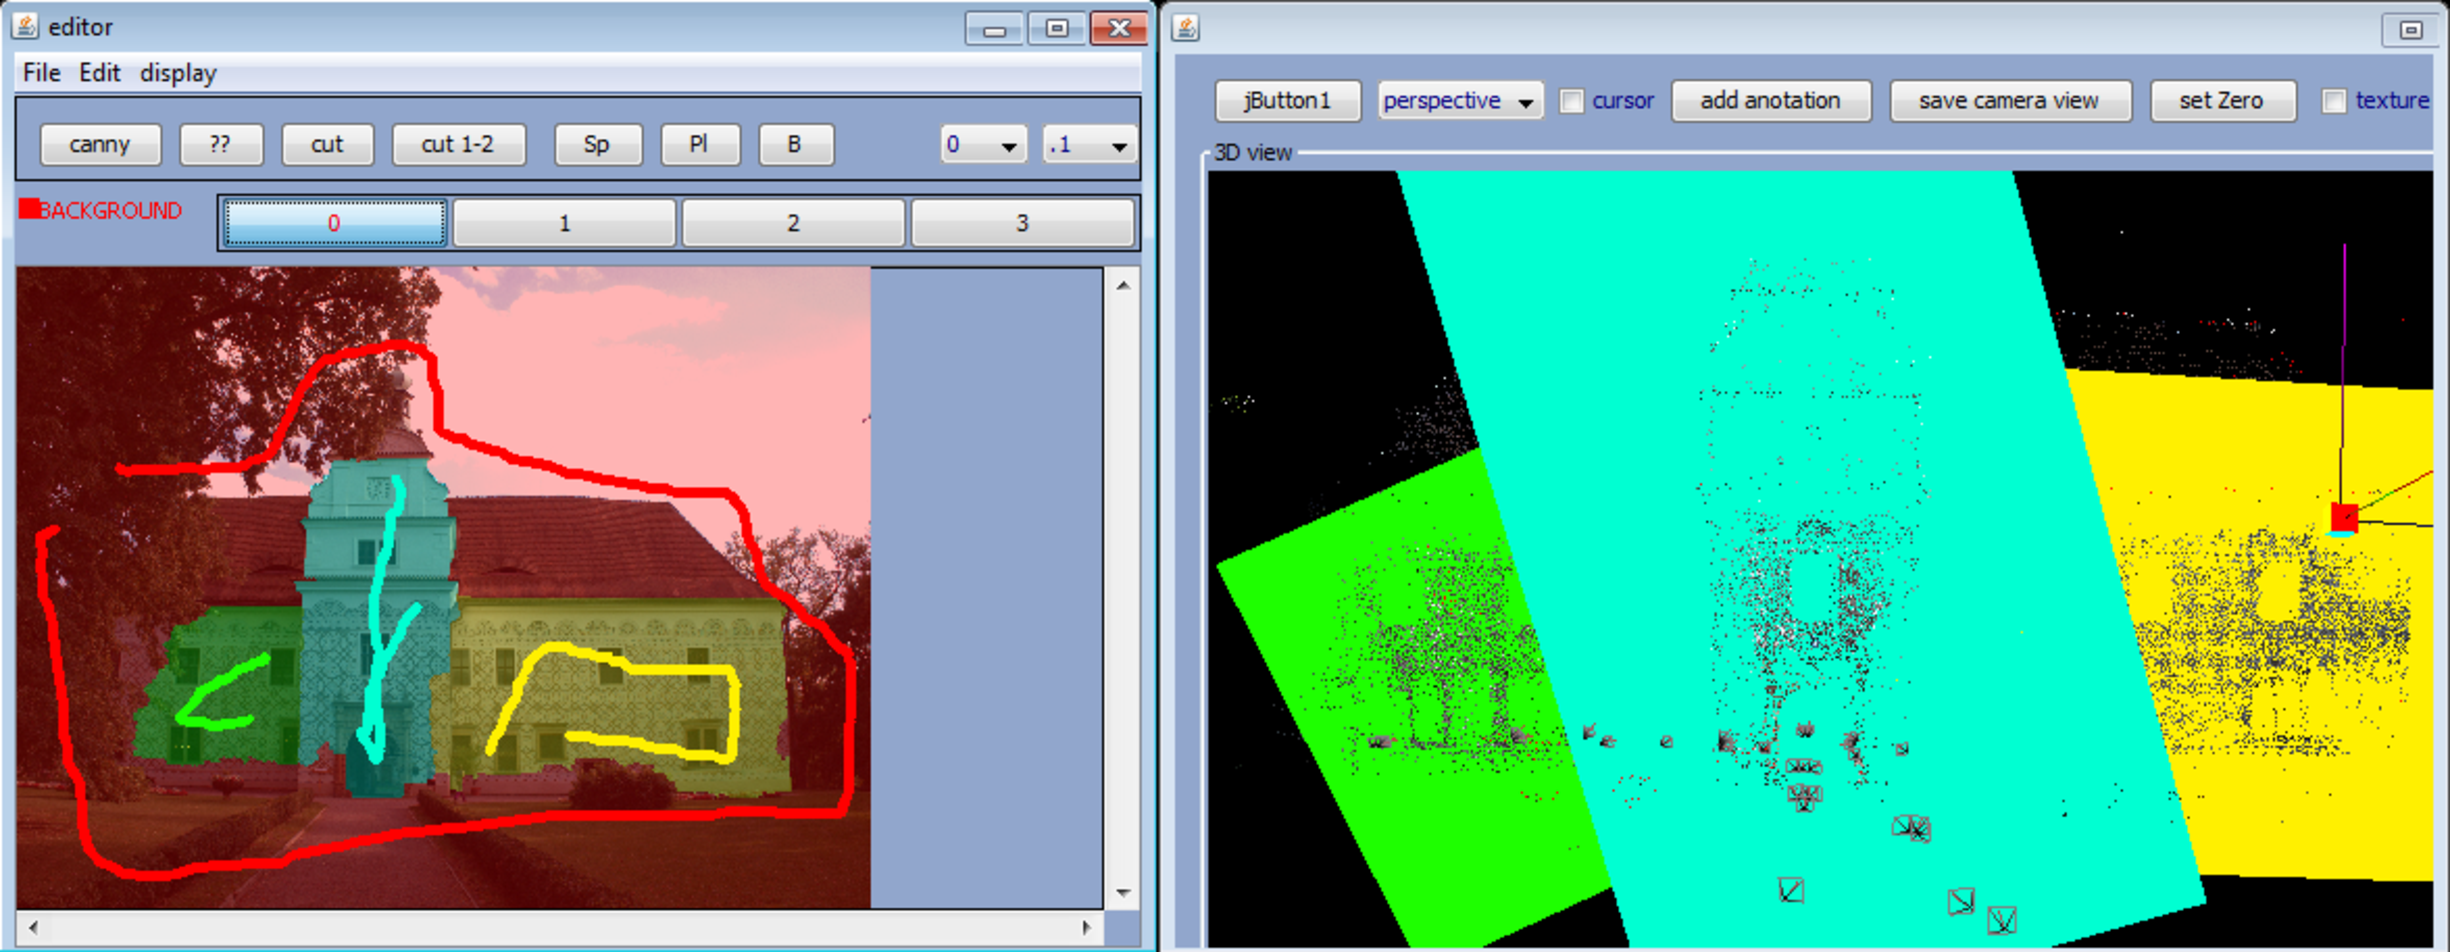
\includegraphics[width=15cm]{ilustrace/program/P-1}
		\caption{Ilustrace vytváření ploch. Uživatel v editoru (vlevo) zadal data pro 3 plochy (žlutá, zelená tyrkysová). Tyto plochy jsou zobrazeny ve 3D scéně (vpravo) }
		\label{fig:P-1}
	\end{center}
\end{figure}

\begin{figure}[]
	\begin{center}
		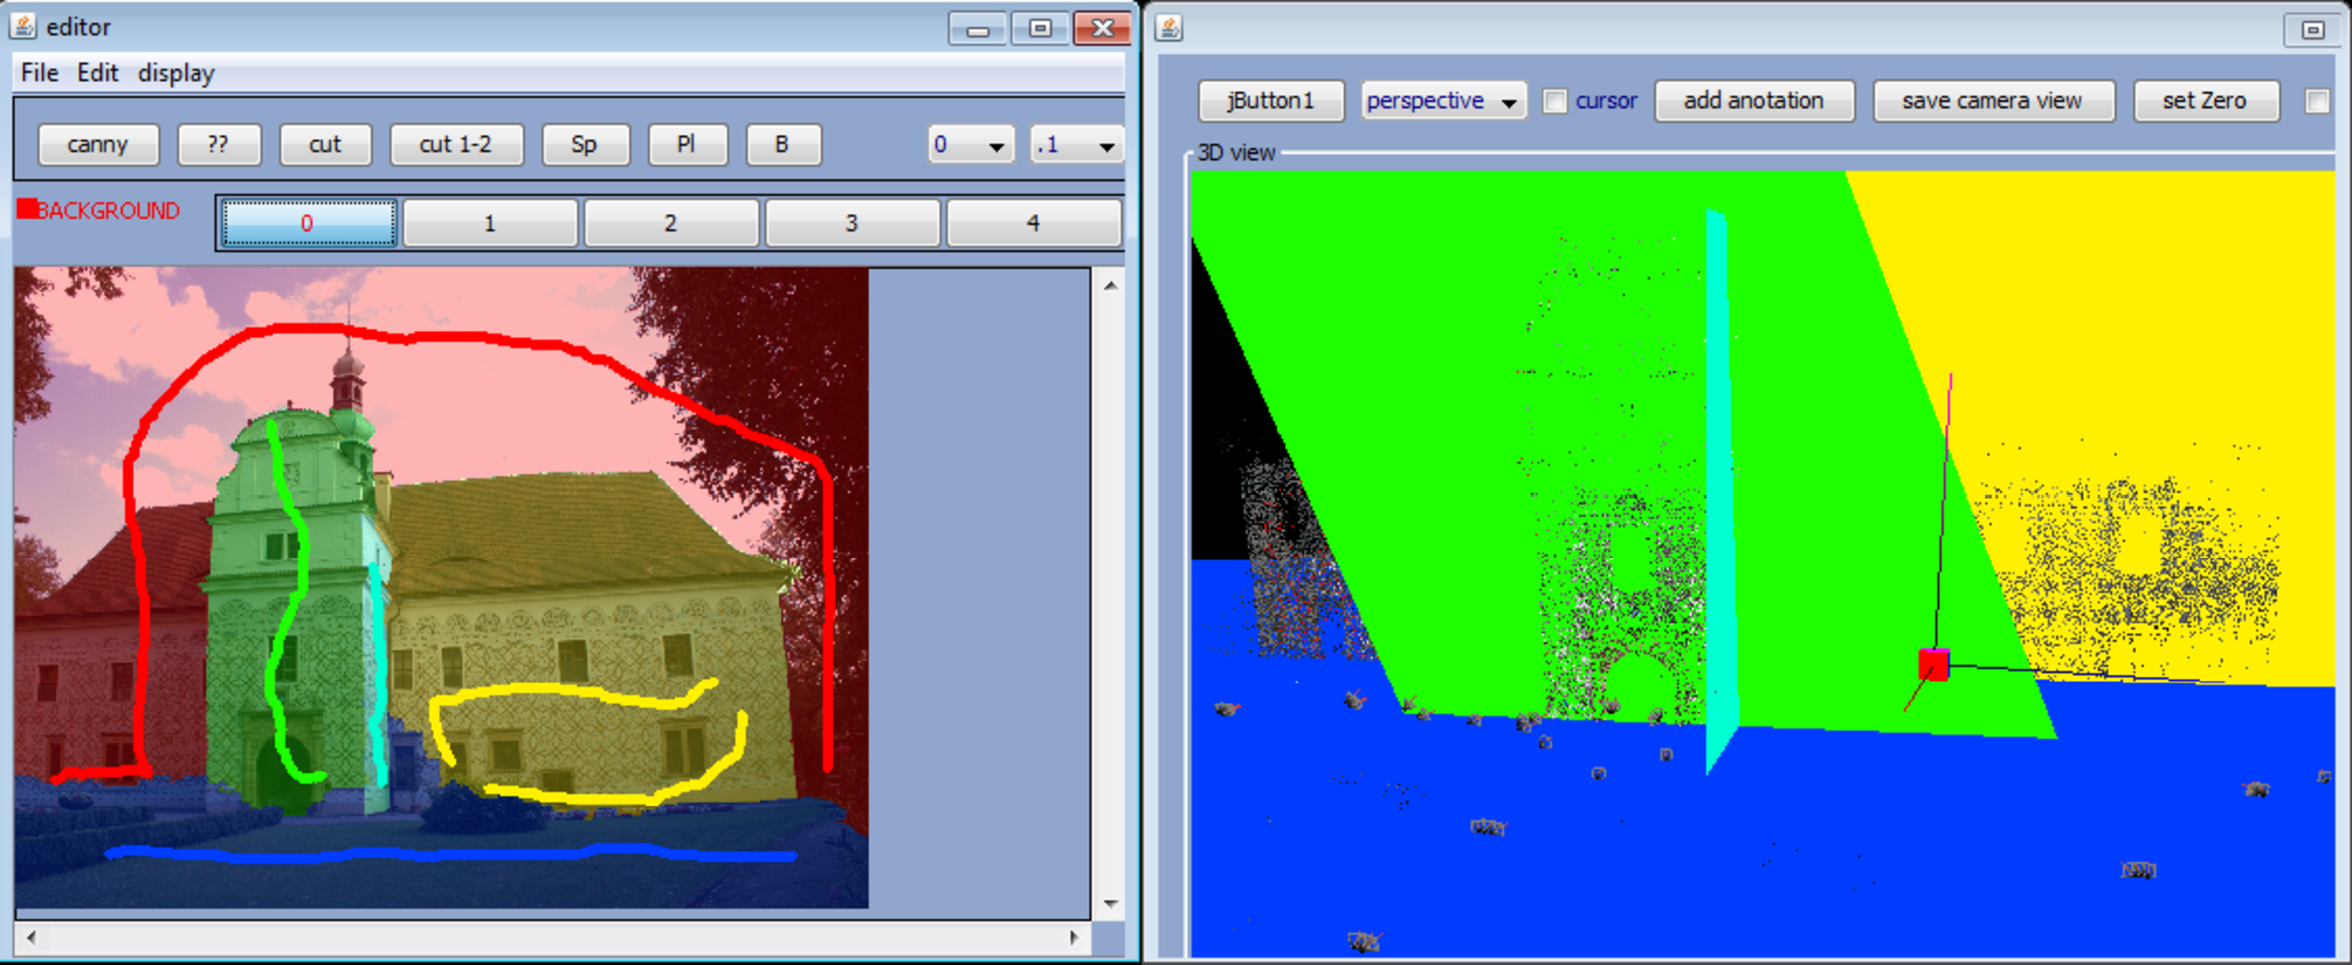
\includegraphics[width=15cm]{ilustrace/program/P-2}
		\caption{Ilustrace ořezávání ploch mezi sebou. Zde je možné vidět editor se zadanými daty pro 4 plochy do fotografie (vlevo) a 3D scénu kde tmavě modrá plocha ožezává žlutou, tyrkysovou a zelenou plochu (vpravo) }
		\label{fig:P-2}
	\end{center}
\end{figure}

\begin{figure}[]
	\begin{center}
		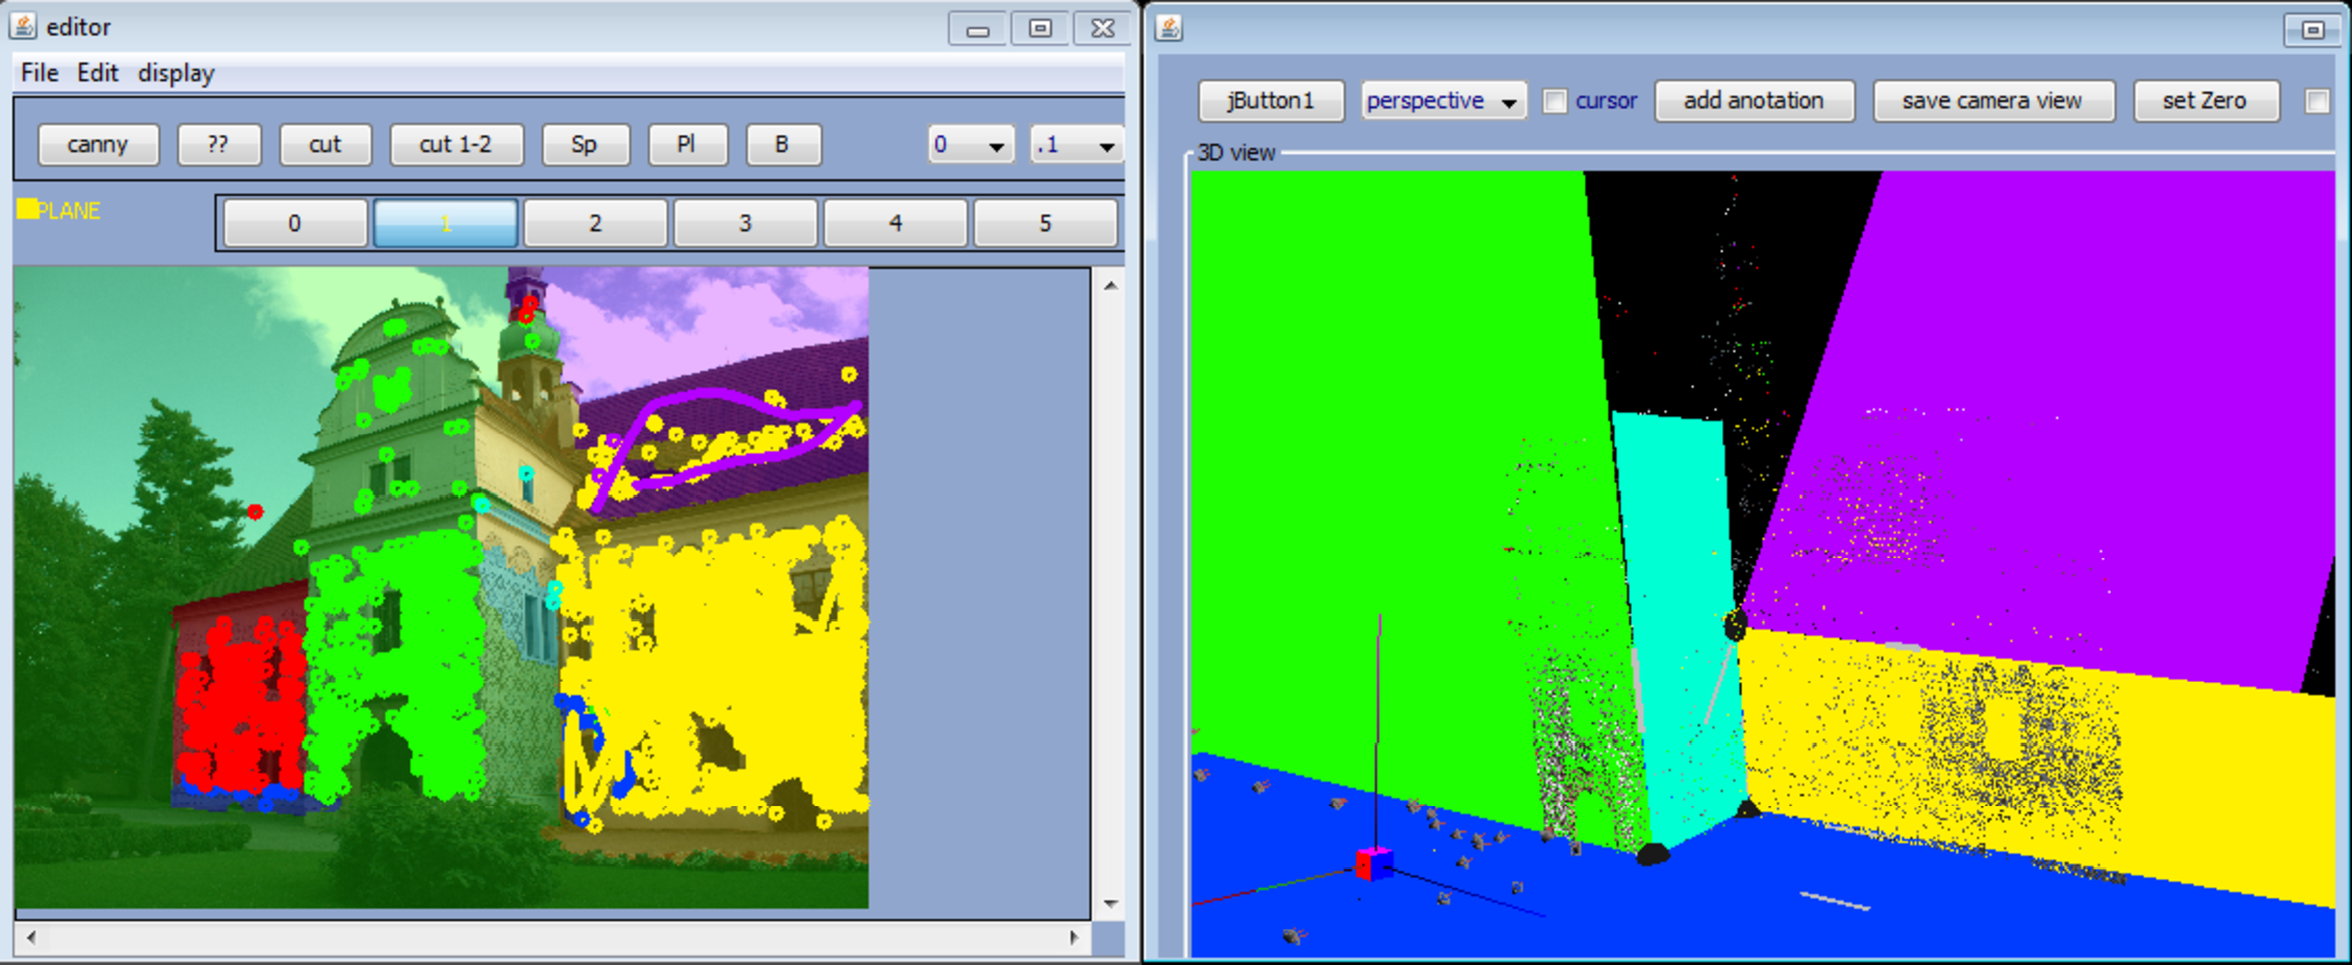
\includegraphics[width=15cm]{ilustrace/program/P-3}
		\caption{Ilustrace ořezávání ploch mezi sebou. Zde je možné vidět editor se zadanými daty pro 5 plochy do fotografie (vlevo) a 3D scénu kde jsou tyto navzájem se ořezávající plochy zobrazeny. }
		\label{fig:P-3}
	\end{center}
\end{figure}

\clearpage


\section{Důležité komponenty aplikace}
V této části se nachází popis základních tříd programu ArchiRec3D. Jsou zde popsány pouze větší třídy týkající se řešených problémů (\ref{cil}) 

\subsection{MDI\_pc\_gis}
Tato třída slouží ke spuštění celé aplikace. Při spuštění programu vytvoří hlavní okno a k němu vytvoří všechna další okna, která budou uživatelem používána. Okna, která jsou v tomto kroku vytvořena, jsou: Editor (třída MDI\_editor\_v1), 3D scéna (třída MDI\_pc\_3D), Info (třída MDI\_Info)a Log (třída MDI\_Log). Zároveň jsou tyto komponenty uloženy do statických proměnných třídy MDI\_app\_state.
\paragraph{} 
Tato třída také uživateli poskytuje možnost načítat data. Například scénu získanou programem Bundler. Načítání této scény je realizováno třídou BundlerLoader.

\subsection{BundlerLoader}
Třída realizující načítání dat získaných programem Bundler. Tato třída je jedním z řady loaderů použitých v aplikaci. Ze složky se scénou otevře soubor "bundle.out" a jeho obsah rozparsuje a uloží. Z tohoto souboru získá počet kamer, jejich transformace, ohniskovou vzdálenost a radial distortion parametry. Dále získá množinu 3D bodů, kde každý bod je reprezentován svou pozicí, barvou a seznamem kamer a pozic. Kamera je v seznamu, pokud v jí odpovídající fotografii byl bod nalezen a pozice odpovídá místu v dané fotografii. Dále je ze souboru "list.txt" získán seznam fotografií, které odpovídají kamerám (v daném pořadí). 

\subsection{MDI\_Info}
Třída pro vytvoření a obsluhu info okna. Toto okno obsahuje seznam fotografií, který je uživateli zobrazen jako seznam jejich názvů. Uživatel má možnost vybrat libovolnou z nich kliknutím na její jméno. Vybrání fotografie způsobí, že fotografie se nastaví jako aktuální ve statických proměnných třídy MDI\_app\_state, fotografie se zobrazí v editoru, a pokud je nastavena možnost LookThrough, použije se pro kameru pohledu transformace kamery, ze které byla daná fotografie vyfocena. Pokud uživatel kurzorem ukáže na název fotografie bez kliknutí, jsou zobrazeny informace o fotografii. Pokud je v danou chvíli vybrána jiná fotografie, zobrazí se informace o vztahu mezi fotografiemi. Informace obsahují zmenšený náhled fotografie, její název, počet bodů, které byly v této fotografii nalezeny při rekonstrukci a pokud už byla uživatelem vybrána nějaká fotografie, je zde zobrazeno kolik zaregistrovaných bodů tyto fotografie sdílí.

\subsection{MDI\_editor\_v1}
Třída pro vytvoření a obsluhu okna editoru fotografie. V okně tvořeném touto třídou je zobrazena uživatelem vybraná fotografie a uživatel s ní může manipulovat. Uživatel může například zvětšit nebo zmenšit fotografii, provést její rotaci o násobky 90 stupňů nebo ji posunout. Kromě fotografie si uživatel může nechat zobrazit dodatečné informace, jako například body zaregistrované v zobrazené fotografii, nebo segmentaci fotografie. 
\paragraph{}

\subsection{MDI\_app\_state}
Tato třída je vlastně kolekcí statických metod a statických proměnných. Udržuje se v ní uložen veškerý stav aplikace. Všechna okna, projekt, scéna, nastavení projektu a aplikace, uživatelem vybraná fotografie, instance všech kamer, instanci třídy SegmentationWrapper a další důležité komponenty. Tento způsob uložení dovoluje všem třídám přístup k datům scény a umožňuje komunikaci mezi jednotlivými komponentami.
\paragraph{}
Obsahuje především metody pro ukládání stavu jednotlivých oken (při ukončení aplikace se ukládá rozmístění, velikost a další informace o oknech) a také metody pro aktualizaci jednotlivých komponent programu\footnote{Například po vybrání jiné fotografie je nezbytné aktualizovat fotografii zobrazenou v editoru a změnit pohled ve 3D scéně, nebo po provedení segmentace fotografie je nutné vygenerovat nové plochy a zobrazit je ve 3D scéně}.

\subsection{MDI\_pc\_3D}
Tato třída slouží k vytvoření a obsluze okna s 3D scénou. Zobrazená scéna je složena z mračen bodů, kamer a ploch. Mračno bodů odpovídá bodům, které byly získány z importované scény. Kamery odpovídají kamerám importované scény a jsou reprezentovány jednoduchými objekty, které ukazují pozici a směr pohledu kamery. Plochy jsou zde reprezentovány barevnými\footnote{Barva je závislá na indexu plochy, tj. je závislá na pořadí, v jakém jsou plochy uživatelem přidány.} obdélníky. Scéna také může obsahovat body a anotace. Body z výše zmíněného mračna je možné vybrat kliknutím myši, pokud je zaškrtnuta možnost "cursor". Takto vybraný bod je označen a v tuto chvíli je možné tomuto bodu přidat anotaci, což je vlastně popisek, který se bude zobrazovat ve 3D scéně. Dále je zde možnost měřit vzdálenost mezi body. Měření se provádí tehdy, je-li kromě možnosti "cursor" zaškrtnuta i možnost "measure". Následně scéna udává informace o vzdálenosti mezi dvěma za sebou vybranými body ve scéně. Tato vzdálenost nereprezentuje skutečné vzdálenosti reálného objektu. Nástroj "set" umožňuje uživateli změnit měřítko scény. Pokud uživatel změřil vzdálenost mezi nějakými body ve scéně, je touto volbou uživateli zobrazeno, jak veliká tato vzdálenost je a uživatel má možnost aplikaci říci, na jakou hodnotu tuto vzdálenost chce nastavit. Tím dojde ke zvětšení/změnšení scény. Změna měřítka celé scény způsobí změnu v chování pohybu kamery. Uživatel má možnost svou kamerou ve scéně pohybovat a tím měnit pozici, ze které pozoruje scénu. Kamerou je možné posunout podél jejích os (pohyb v rovině XY pohybem myši a po ose Z kolečkem myši, vše v souřadnicích kamery), nebo rotovat kolem počátku scény. Vzdálenost, o kterou se kamera posune, ale není závislá na velikosti scény, tudíž ve větší scéně se bude zdát, že se kamera pohybuje pomaleji. 

\subsection{MDI\_Log}
Třída pro vytvoření a obsluhu okna s logem. V okně se zobrazují informace o tom, co program vykonal spolu s dalšími informacemi o provedené akci. Třída obsahuje pouze pár metod pro vložení textu do logu s ukazateli, zda je to informační text, error, nebo nějaký jiný typ textu.

\subsection{Image}
Tato třída reprezentuje fotografii, která patří k načtené scéně. Každá instance si uchovává rozměry fotografie, url, množinu 2D bodů, které byly v této fotografii zaregistrovány a odkaz na kameru, ze které byla fotografie získána.

\subsection{PinholeCamera}
Instance této třídy reprezentují jednotlivé kamery patřící ke scéně. V proměnných jsou udržovány informace jako translace, rotace nebo ohnisková vzdálenost. Zároveň si v jedné proměnné udržuje odkaz na fotografii (Image), který této kameře odpovídá. 

\subsection{SegmentationWrapper}
Tato třída slouží k odstínění uživatele od samotné segmentace fotografie. Nejdůležitější metody této třídy jsou segmentation a rebuildSceneAfterSegmentation. První z těchto metod deleguje segmentaci fotografie na konkrétní implementaci\footnote{Tříd řešících segmentaci fotografie je v aplikaci několik, všechny ale sdílejí interface GraphCutSegmentation}. Druhá metoda slouží k tomu, aby byla znovu vytvořena 3D scéna. K této metodě se také váže metoda reconstructPlane. V této metodě se nejprve pomocí instance třídy RansacPlaneFitting získá rovina odpovídající bodům ze segmentace. Následně se rovina uloží do instance třídy CSG\_Plane odpovídající této ploše a nakonec je do té samé instance uložena i geometrie této plochy získané pomocí metody findBestVisualisation4 třídy Plane3DUtils.

\subsection{RansacPlaneFitting}
Tato třída slouží k tomu, aby pro množinu 3D bodů byla nalezena co nejlepší možná rovina. K získání této roviny využívá ransac algoritmus.

\subsection{Plane3DUtils}
Tato třída obsahuje sadu statických metod pro práci s rovinami a pro vytváření geometrií. Jednou z nejdůležitějších metod této třídy je metoda findBestVizualization4, který slouží k vytvoření geometrie plochy z množiny bodů a roviny, ve které tato plocha má být. Tato metoda promítne výše zmíněnou množinu bodů do roviny a následně vytvoří nejmenší obalové těleso. Dále je zde například metoda getTransformFromPlaneToPlane001 který vytvoří transformaci takovou, že body ze zadané roviny budou transformovány do roviny xy. Tato metoda je využívána například ve výše zmíněné findBestVizualization4.

\subsection{Project}
Tato třída reprezentuje právě otevřený projekt. Při spuštění aplikace je projekt prázdný a každá další načtená scéna se do něj ukládá. Instance této třídy obsahuje především list instancí třídy SceneTr. Všechny scény, které projekt obsahuje, jsou zobrazeny ve 3D scéně, ale uživatel může pracovat v jednu chvíli pouze s jediným projektem.

\subsection{SceneTr}
Tato třída reprezentuje jednotlivé načtené scény. Nová instance se vytváří při každém importování nové scény a je přidána do projektu. Třída obaluje množiny mračen bodů, transformaci celé scény a jednu instanci třídy CSG .

\subsection{CSG}
Tato třída slouží jako kontejner pro množiny CSG objektů (CSG\_Plane, CSG\_Line, CSG\_Point, CSG\_Sphere), které patří k jedné konkrétní scéně. Třída obsahuje metody pro přístup k celým kolekcím s objekty nebo i k jednotlivým objektům (například přístup k instancím CSG\_Plane pomocí indexů ploch).

\subsection{CSG\_Plane}
Tato třída reprezentuje jednu konkrétní plochu. Obsahuje jak rovinu, která dané ploše odpovídá, tak i její geometrii reprezentovanou objektem GeometryArray\footnote{Instance této třídy uchovává informace o vrcholech, hranách a plochách trojrozměrného tělesa. Z GeometryArray se následně vytváří objekt, který se připojí ke grafu scény a je vykreslen v 3D scéně.}\cite{Java3DDoc}. Dále třída obsahuje barvu plochy a index této plochy. Index plochy odpovídá pořadí jejího vytvoření, kde první plocha má index 1.

\subsection{CSG3D}
Tato třída slouží jako kolekce statických metod pro vytváření konkrétních objektů, které budou zobrazeny ve 3D scéně z jednotlivých CSG objektů (CSG\_Plane/Line/Point/Sphere). Obsahuje především metodu createPlane, která z instance třídy CSG\_plane vytvoří zobrazitelný objekt. Tato metoda také vytváří materiál pro objekt a určuje, jakým způsobem bude výsledné těleso zobrazeno (zda těleso bude vyplněné nebo třeba pouze wireframe).

\clearpage

\begin{figure}[h]
	\begin{center}
		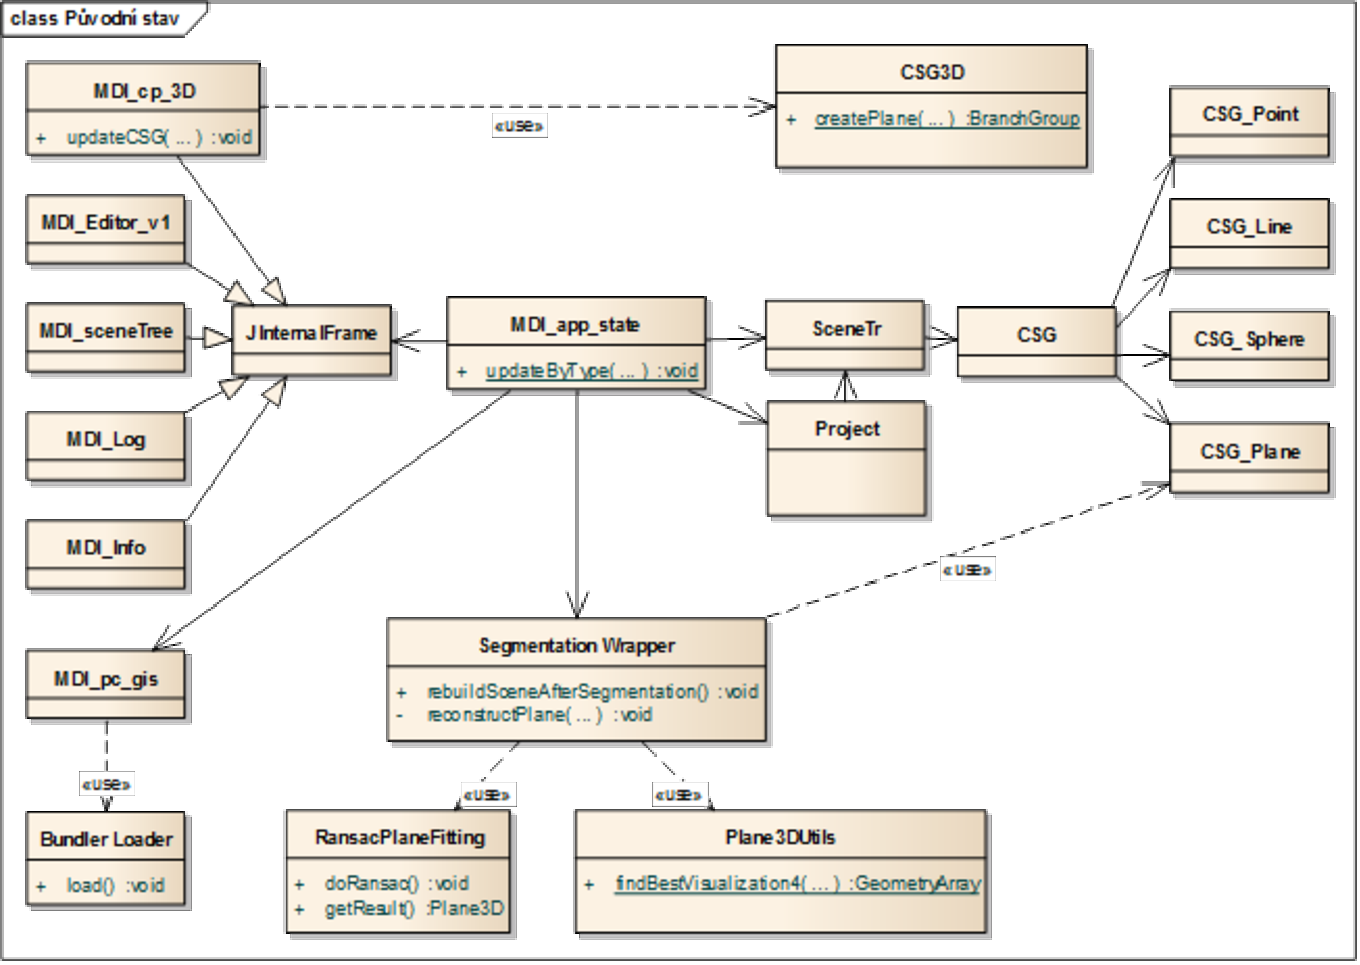
\includegraphics[width=15cm]{ilustrace/StateBefore}
		\caption{Ilustrace znázorňující základní třídy programu a jejich propojení mezi sebou.\protect\footnotemark}
		\label{fig:stateBefore}
	\end{center}
\end{figure}

\footnotetext{Tento diagram je značně zjednodušený. Jsou zde zobrazeny pouze třídy které souvisejí s problémy řešenými v této práci. Zároveň jsou vynechány atributy jednotlivých tříd a prakticky většina jejich metod. U tříd jsou zobrazeny pouze významené metody které jsou v textu této práce zmíněny. Pokud zobrazené metody mají parametry, jsou nahrazeny "...". Tato zjednodušení byla provedena v zájmu přehlednosti diagramu a aby nemusel být dělen na menší části.}


\section{Vytváření ploch}
\label{vytvareniPlochy}
Geometrie reprezentující plochy, které budou následně vykresleny ve 3D scéně, jsou uloženy v objektech třídy CSG\_Plane. Všechny tyto objekty jsou uloženy v instanci třídy CSG, která obaluje všechny ostatní objekty pro vykreslování ve 3D scéně. Instance CSG je uložena v instanci třídy SceneTr. Instance SceneTr je dostupná přes statickou proměnnou třídy MDI\_scene\_app. 
\paragraph{}
V aktuálním stavu je pro vytvoření ploch volána metoda rebuildSceneAfterSegmentation na instanci třídy Segmentation Wrapper. Zde je pro každou plochu zavolána metoda reconstructPlane s indexem plochy a množinou bodů, která patří dané ploše. 
\paragraph{}
V reconstructPlane je pomocí instance třídy RansacPlaneFitting získána rovina, která odpovídá zadaným bodům. Následně se z MDI\_app\_state získá instance CSG\_Plane s indexem odpovídajícím zadané hodnotě a je zavolána metoda findBestVisualisation4, jejíž výsledná geometrie (instance třídy GeometryArray) je uložena do dříve získané instance CSG\_Plane.

\begin{figure}[h]
	\begin{center}
		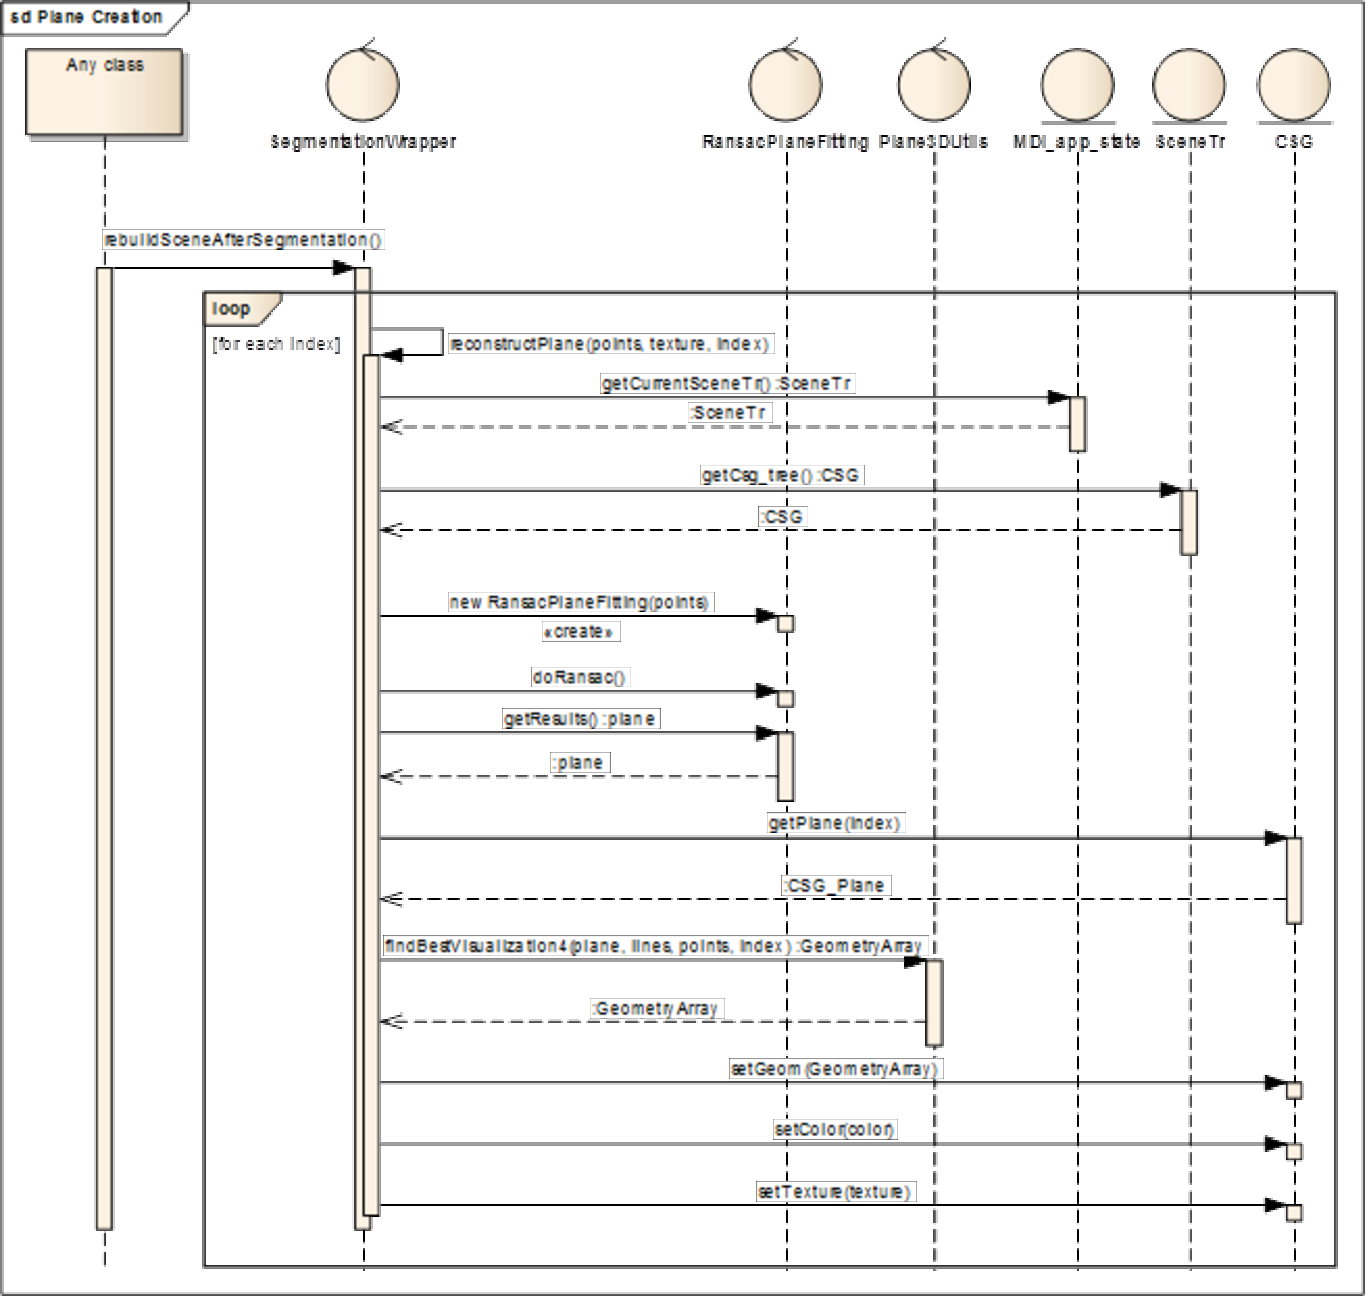
\includegraphics[width=15cm]{ilustrace/PlaneCreation}
		\caption{Diagram znázorňující rekonstrukci ploch po segmentaci}
		\label{fig:stateBefore}
	\end{center}
\end{figure}

\paragraph{}
V mětodě findBestVisualisation4 je nejprve vytvořena transformace T. Tato transformace je taková, že rovinu, jež byla metodě předána jako parametr (ta, jež byla získána pomocí instance třídy RansacPlaneFitting), transformuje do roviny $XY$. Což znamená, že když se tato transformace aplikuje na body v prostoru, jejich souřadnice Z bude označovat vzdálenost bodu od roviny. Tuto transformaci aplikujeme na body.  Poté je provedeno vynulování souřadnice $z$ u všech transformovaných bodů (jelikož by body měly odpovídat jedné rovné rovině a rovina je proložena těmito body, souřadnice $z$ by měla být minimální). Následně je vytvořeno obalové těleso pro množinu bodů. Pokud se jednotlivé plochy mají mezi sebou ořezávat, vezmou se přímky odpovídající průsečíkům jejich rovin. Pokud program nemá dostatečné množství přímek, jsou nalezeny $min$ a $max$ hodnoty souřadnic $x$ a $y$ bodů. Tyto hodnoty se zvětší a použijí se pro vytvoření přímek, které ve výsledku vytvoří obdélník kolem bodů. 
\paragraph{}
Když už je dostatek přímek, jsou nalezeny průsečíky přímek, přímky jsou rozděleny na segmenty. Tyto segmenty jsou ohodnoceny a je nalezena uzavřená cesta taková, že těleso, kterému je tato cesta hranicí, obsahuje všechny body a je nejmenší možné. Následně je na body definující tuto cestu aplikována inverzní transformace k transformaci T. Jelikož měly tyto body souřadnici $z$ rovnu nule, výsledné body budou v jedné rovině. Tyto body jsou poté vloženy do instance třídy GeometryInfo, která z nich vyrobí GeometryArray. GeometryArray je následně uložen do objektu odpovídající plochy. Z tohoto objektu se při vytváření 3D scény vytváří těleso, které je přidáno do grafu scény \footnote{Podrobnější informace o grafu scény v Java 3D Programming \cite{Java3DGuide}, kapitola 4} . 

\section{Importní modul pro VisualSFM}
\label{analyzaStart}
Jedním z cílů práce je vytvořit modul, jenž dovolí uživateli importovat do programu scénu získanou programem VisualSFM. 

\subsection{Účel modulu}
Aby uživatel mohl začít s programem pracovat, je nezbytné nejdřív importovat scénu. Data této scény jsou následně použita spolu se vstupy od uživatele pro vytváření trojrozměrného objektu, který bude reprezentovat rekonstruovaný objekt. Ve stávajícím stavu program dovoluje importovat pouze scénu generovanou programem Bundler, který je poměrně těžkopádný na použití. Program VisualSFM je k uživateli více přívětivý.

\subsection{Bundler a VisualSFM}
Oba tyto programy slouží k 3D rekonstrukci využívajíc Structure from Motion(viz. \ref{SFM}) Oba dva programy využívají jako vstup neuspořádanou množinu fotografií. Výstupem je adresář obsahující scénu a další dodatečná data.

\subsection{Structure from Motion}
\label{SFM}
Jde o způsob 3D rekonstrukce objektu podle fotografií, které rekonstruovaný objekt zachycují z různých úhlů. Podrobnější informace je možné získat například z Robust structure from motion using motion parallax\cite{Cipo}.

\subsection{Vstupní data programu}
Prostudováním výstupních dat z obou programů jsem došel k závěru, že rozdíl mezi výstupními daty obou programů je velmi malý. Základní soubor obsahující data ohledně kamer a bodů získaný z programu Bundler je "./bundle/bundle.out" a využívá formát "Bundle file v0.3". V datech z programu VisualSFM se informace o kamerách nacházejí v souboru "./bundle.rd.out" a mají naprosto stejný formát "Bundle file v0.3". Další data nezbytná pro scénu je seznam fotografií, které jsou v dané scéně použity a fotografie samotné.  Ve výstupu programu Bundler je seznam uložen v souboru "./list.txt" a obsahuje na začátku každého řádku cestu k fotografii a následně další parametry oddělené mezerami. Ve výstupu z programu VisualSFM je list uložen na stejném místě se stejným jménem. Jediný rozdíl je, že cesty k fotografiím nejsou násedovány výčtem parametrů, což ale nevadí, neboť tyto parametry ArchiRec3D nepoužívá. Další data, která program ještě používá, jsou klíčové body (viz. \ref{keypoints}), které jsou uloženy v souborech "*.key.gz", kde * je název fotografie, ke které klíčové body patří\footnote{k fotografii "test.jpg" bude patřit soubor s klíčovými body "test.key.gz"}. Tyto soubory ovšem výstup z programu VisualSFM neobsahuje.
\paragraph{}
Tato data se používají, když uživatel zvolí v editoru fotografie možnost zobrazit keypointy. Keypointy jsou poté vykreslovány do fotografie, ale nikde jinde se nepoužívají, a tudíž nijak neovlivňují segmentaci, rekonstrukci ani jiné důležité funkce programu. Program je zároveň ošetřen a kontroluje, zda tyto soubory existují před jejich načítáním, takže pokud chybějí, nenastane žádná komplikace.

\subsection{Klíčové body}
\label{keypoints}
Klíčové body jsou dvojrozměrné body, které byly ve fotografiích nalezeny při vytváření scény. Tyto body jsou poskytnuty pouze ve scéně generované programem Bundler. Klíčové body nejsou pro správnou funkci programu ArchiRec3D vyžadovány.

\section{Nástroj pro vytváření hranic ploch}
Jak již bylo v úvodu zmíněno, jedním z nových nástrojů programu bude nástroj pro vytvoření hranice ploch. 

\subsection{Aktuální stav programu}
V aktuálním stavu aplikace uživatel může do scény přidávat plochy, které prokládají množiny trojrozměrných bodů. Plocha ve scéně reprezentována obdélníkem, případně jiným tvarem, pokud se mezi sebou plochy ořezávají. Velikost tohoto útvaru je závislá na rozměrech kolmého průmětu množiny bodů, které této ploše patří, do roviny, ve které se tato plocha nachází\footnote{Vezmou se minimální a maximální hodnoty $x$ a $y$ souřadnic bodů. Tyto maxima a minima se následně upraví tak, aby výsledné těleso bylo větší než množina. Následně se z obdélníku tvořeného těmito body a z přímek pro ořezávání roviny vytvoří výsledný objekt plochy.}.
\paragraph{}
Toto není příliš vhodné, pokud by uživatel chtěl reprezentovat nějaké složitější útvary. Kromě toho je při každé úpravě scény nezbytné znovu vypočítat nejlepší hranice všech ploch ve scéně. Při větším množství ploch, které se mezi sebou vzájemně ořezávají, značně roste náročnost jedné aktualizace scény a aplikace se výrazně zpomaluje. 

\subsection{Cíl}
Mým cílem je tedy vytvořit nástroj, který by uživateli dovolil vytvořit plochu, jejíž tvar by přesně odpovídal uživatelovu přání. Na druhou stranu je potřeba vytvořit nástroj, který by byl pro uživatele pokud možno jednoduchý k použití, aby uživatele neodradil od používání programu a aby byla práce s programem efektivní. 

\subsection{Možnosti zadání hranice}
Jednou z možností je dát uživateli sadu primitiv, ze kterých by si mohl složit výslednou plochu. Reálné objekty ale většinou nemívají naprosto přesný tvar, který by odpovídal čtvercům, obdélníkům nebo třeba trojúhelníkům. Zároveň uživatel by tyto objekty zadával do fotografie, kde jsou objekty díky perspektivě zkresleny. To by ale znamenalo, že by uživatel musel tyto objekty nějakým způsobem upravovat/deformovat, protože by nebylo možné mu zajistit všechny možné tvary. Tyto úpravy by zvýšily náročnost zadávání hranice.
\paragraph{}
Další, pro uživatele mnohem příjemnější, možnost zadávání hranice by mohla být kreslením do scény. Toto by bylo pro uživatele poměrně přirozené a zajistilo by to uživateli, že hranice bude přesně odpovídat jeho přáním. Takto by byla hranice plochy velmi podrobná. I kdyby uživatel kreslil přímku, která by šla reprezentovat jen dvěma body, byla by reprezentována mnohonásobně větším množstvím bodů. Každý z těchto bodů by musel být při každé změně scény promítnut do roviny a výsledná geometrie plochy by byla také zbytečně velmi složitá. Zároveň by byl značný problém pro uživatele upravovat stávající hranici, kdyby během kreslení udělal nějakou chybu.
\paragraph{}
Způsob zadávání, který by odstranil nevýhody toho předchozího, by bylo zadávání pouze menšího množství bodů klikáním do fotografie. Tímto způsobem by uživatel zadal body pouze tam, kde je to potřeba. Tato možnost by také zvýšila přesnost rovných čar, které jsou v architektuře velmi častým jevem, ale snížila by se snadnost zadávání zakulacených hranic. Uživatel by musel zadat větší množství bodů. Na druhou stranu, přesnost by byla větší, neboť uživatel by měl čas v průběhu zadávání fotografii transformovat\footnote{zvětšit/zmenšit nebo posunout}, aby si zjednodušil zadávání. Zároveň by uživatel mohl zvolit, jak podrobně chce danou zakulacenou hranici reprezentovat. 

\subsection{Uložení hranice plochy}
\label{hraniceUlozeni}
Když bude uživatel body zadávat klikáním do fotografie, získáme uspořádanou množinu bodů. Hranice bude tvořena uzavřenou cestou úseček, které získáme spojováním každých dvou po sobě jdoucích bodů a prvního s posledním.  Zároveň aby mohla nějaká hranice být vytvořena, bude nezbytné, aby uživatel zadal alespoň 3 body, neboť trojúhelník je nejmenší\footnote{Nejmenším je zde myšleno těleso tvořeno nejmenším množstvím vrcholů.} možné těleso s plochou. Množina bodů tedy musí být uspořádaná a musí mít nejméně 3 prvky, jinak bude muset být použita neoříznutá plocha jako se tomu děje teď.
\paragraph{}
Zároveň bude nezbytné uložit si informaci o tom, ke které ploše daná množina bodů patří. Jelikož všechny body jedné množiny patří jedné ploše, není třeba, aby si každý bod udržovat tuto informaci. Toto propojení mezi množinou a plochou by bylo možné udržovat například tak, že každá množina by si ukládala index, který je pro každou plochu jedinečný. To by ale neřešilo problém, kam množinu uložit. Dále by šlo použít kolekci, kde by pro každou plochu byla uložena tato množina pod jejím indexem. Toto by ale vyžadovalo kolekci uložit na místo, kde by všechny třídy, které množiny bodů budou využívat, měli ke kolekci přístup. Zároveň tyto množiny, reprezentující hranice, jsou vlastnostmi jednotlivých ploch. Proto by bylo jistě výhodnější, aby tyto množiny byly uloženy u ploch, ke kterým patří. Instance třídy reprezentující plochy jsou přístupné díky třídě MDI\_app\_state.

\subsection{Model kamery}
\label{modelKamery}
V aplikaci je pro kameru použit Pinhole camera model\cite{MultipleViewGeometry} \cite{CameraModel}.  Uvažujeme tedy, že kamera nemá žádnou čočku a clona má v sobě nekonečně malý otvor, který propustí pouze jeden paprsek světla. 
\paragraph{}
Model (obr. \ref{fig:cameraModelA}) funguje tak, že máme optickou osu $o$ , což je přímka v prostoru. Na optické ose se nachází střed kamery $S$. Střed kamery odpovídá onomu malému otvoru v cloně. Optická osa bude shodá s osou $z$. Dále máme obrazovou rovinu $a$, která je rovnoběžná s rovinou $XY$, tj. je kolmá k optické ose. Obrazová rovina $a$ se nachází ve vzdálenosti $f$ od středu kamery, kde $f$ je ohnisková vzdálenost kamery.
\paragraph{}
Každý přicházející paprsek prochází středem kamery a dopadá na obrazovou rovinu $a$, kde vytváří obraz. Tento obraz je převrácený podle os $x$ a $y$ (jako počátek souřadného systému obrazu bereme průnik optické osy a obrazové roviny $a$, kde osa $z$ odpovídá směru optické osy). Velikost obrazu je přímo úměrná ohniskové vzdálenosti.

\begin{figure}[h]
	\begin{center}
		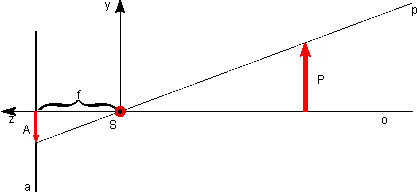
\includegraphics[width=10cm]{ilustrace/Il-3-1}
		\caption{Ilustrace Pinhole camera modelu. $O$ - optická osa, $z$ - osa $Z$, $y$ - osa $Y$, $f$ - ohnisková vzdálenost, $a$ - obrazová rovina, $S$ - střed kamery, $P$ - objekt, $A$ - průmět objektu $P$ na $a$, $p$ - promítací paprsek  (osa $X$ směřije k pozorovateli)}
		\label{fig:cameraModelA}
	\end{center}
\end{figure}

Představme si v tomto modelu ještě obrazovou rovinu $b$, rovnoběžnou s původní obrazovou rovinou (obr. \ref{fig:cameraModelB}). Obrazová rovina $b$ je posunuta od středu kamery také o vzdálenost $f$, ale na druhou stranu podle optické osy, než je obrazová rovina $a$. Jelikož tento model nepoužívá žádnou čočku, která by lámala paprsky, všechny přicházející paprsky jsou po celou dobu přímky. V tomto upraveném modelu všechny paprsky nejdříve prochází obrazovou rovinou $b$, na kterém vytvářejí obraz $B$. Následné pokračují dále jako v neupraveném modelu. Takto získaný obraz $B$ je středově souměrný s původním obrazem $A$ podle středu kamery. Obraz $B$ má oproti $A$ tu výhodu, že není převrácený.


\begin{figure}[h]
	\begin{center}
		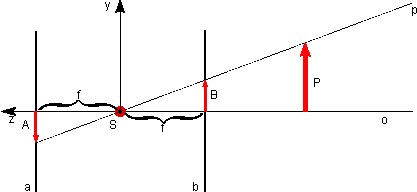
\includegraphics[width=10cm]{ilustrace/Il-4-1}
		\caption{Ilustrace Pinhole camera modelu. $O$ - optická osa, $z$ - osa $Z$, $y$ - osa $Y$, $f$ - ohnisková vzdálenost, $a$ - obrazová rovina, $b$ - přidaná obrazová rovina, $S$ - střed kamery, $P$ - objekt, $A$ - průmět objektu $P$ na $a$, $B$ - průmět objektu $P$ na $b$, $p$ - promítací paprsek  (osa $X$ směřije k pozorovateli)}
		\label{fig:cameraModelB}
	\end{center}
\end{figure}

\subsection{Promítnutí bodu}
Mějme tedy nějaký obraz $B$ v obrazové rovině $b$. Každý bod v obrazu $B$ reprezentuje přímku v prostoru. Vše, co je na této přímce, se v obrazu $B$ stane jediným bodem. Tato přímka prochází svým bodem v obrazu $B$ a středem kamery. Nyní nahraďme obraz $B$ nějakou fotografií z naší scény. Pokud tedy máme do fotografie přidán bod, můžeme snadno najít přímku ve 3D prostoru, po které se onen bod promítá. Stačí nám vzít střed kamery (souřadnice $(0,0,0)$) a bod zadaný do fotografie, kde souřadnice $x$ a $y$ odpovídají souřadnicím bodu ve fotografii vůči středu fotografie (střed fotografie je průsečík obrazové roviny $b$ a optické osy $o$) a souřadnice $z$ bude $-f$, kde $f$ je ohnisková vzdálenost kamery.  Přímka proložená těmito dvěma body bude reprezentovat promítací paprsek. Když tedy budeme promítat nějaký bod z fotografie do roviny, bude stačit vytvořit jeho promítací paprsek a pak spočítat průsečík paprsku s rovinou.

\subsection{Aplikace hranice plochy}
Když už máme plochu, označme si ji jako $R$, a její hranici, bude třeba tuto hranici aplikovat na $R$. Hranici $R$ máme uloženou jako uspořádanou množinu dvojrozměrných bodů. K oříznutí $R$ je ale nezbytné dostat tyto body do prostoru. $R$ je reprezentována jako rovina a množina bodů, které do ní patří. K tomu, abychom mohli body promítnout, potřebujeme informaci o tom, v jaké fotografii byl bod zadán. A pokud tuto informaci budeme udržovat pro každý bod hranice zvlášť, dovolí to uživateli zadávat body pro jednu hranici ve více než jedné fotografii. Toto by mohla být výhoda v případě, že část objektu, který uživatel rekonstruuje, je zakryt jiným objektem\footnote{Například roh budovy může být v jedné fotografii zakryt korunou stromu}.
\paragraph{}
Máme informaci o tom, ve které fotografii je bod zadán. Díky tomu máme informaci o pozici a natočení kamery, neboť každé fotografii odpovídá kamera, ze které byla tato fotografie získána.\footnote{Každé fotografii odpovídá přesně jedna kamera a každé kameře odpovídá přesně jedna fotografie. To také znamená, že pokud máme kameru, máme přístup k její fotografii a obráceně.} Také máme informaci o rovině, ve které leží plocha $R$ a do které potřebujeme získat průmět tohoto bodu. Bod tedy bude stačit promítnout pomocí kamery do této roviny, čímž získáme 3D bod. Když toto provedeme s každým bodem této hranice, získáme množinu 3D bodů, která bude jednoznačně reprezentovat oříznutou plochu $R$.
\paragraph{}
V každém případě bude nezbytné zobrazit v editoru fotografie zadané body i hranici tak, aby uživatel měl informace, kam bod zadal a jaké je jejich pořadí v hranici. 

\begin{figure}[h]
	\begin{center}
		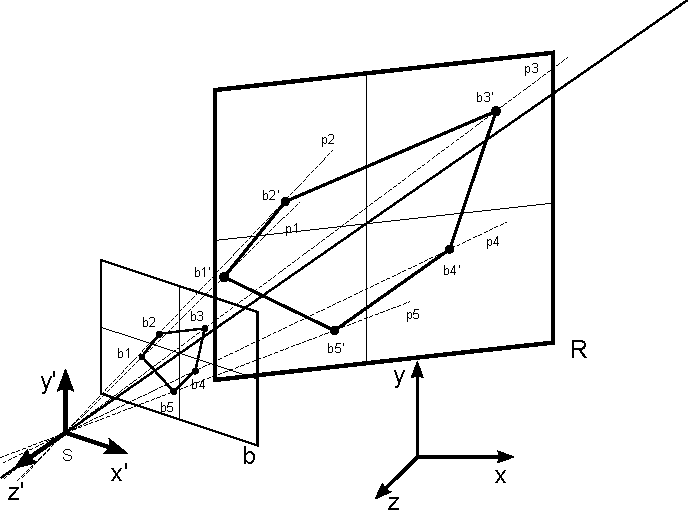
\includegraphics[width=10cm]{ilustrace/Il-10-1}
		\caption{Ilustrace promítání hranice na plochu. $x$,$y$,$z$ - osy světového souřadného systémy, $x'$,$y'$,$z'$ - osy kamerového souřadného systému, $S$ - střed kamery, $b$ - obrazová rovina kamery, $R$ - rovina do které promítáme, $b1$-$b5$ - promítané body, $p1$-$p5$ - promítací paprsky bodů $b1$-$b5$, $b1'$-$b5'$ - body $b1$-$b5$ promítnuté do roviny $R$ }
		\label{fig:10-1}
	\end{center}
\end{figure}

\subsection{Body ve více fotografiích}
Jak už jsem v předchozích odstavcích zmínil, uživatel bude moci zadávat body jedné hranice ve více pohledech/fotografiích.  Toto přináší problém v tom, že jiná fotografie byla focena z jiného místa jinou kamerou. Pokud tedy budeme mít zobrazenou fotografii a daný bod byl zadán v jiné fotografii, nebudeme schopni tento bod zobrazit. Tím pádem bude nezbytné body nejprve promítnout z kamery, která odpovídá fotografii, ve které byly zadány, do roviny plochy a poté zpět do kamery, jejíž fotografie je zrovna zobrazena v editoru. Zároveň by nejspíš bylo vhodné uživateli ukázat, zda daný bod byl v této fotografii zadán, nebo zda je promítnut z jiné fotografie.

\section{Zpřesňování hranice plochy}
Dalším nástrojem, který bude přidán do programu, bude nástroj pro zpřesňování hranice plochy. Primárním účelem tohoto nástroje je umožnit uživateli v případě, že udělal chybu při zadávání bodů, tuto chybu napravit. Dále tento nástroj umožní, že uživatel může nejdříve nepřesně zadat hranice ploch, čímž si zhruba načrtne jejich tvary a až následně přesně umístí zadané body na jejich správné pozice. 

\subsection{Způsob zpřesňování}
Pokud má být uživatel schopen z jiných pohledů (tj. v jiných fotografiích) zpřesňovat hranice ploch, bude nezbytné vytvořit nástroj, který uživateli dovolí změnit pozici daného bodu. To znamená, že uživatel bude muset být schopen nějakým nástrojem vybrat bod, který chce upravit a poté změnit jeho pozici. Nejvýhodnější způsob vybrání bodu, a zároveň i nejpohodlnější pro uživatele, bude kliknutí na bod, který chce vybrat.  Jelikož ale bod zabírá pouze jeden pixel ve fotografii, bude vhodnější vybrat bod nejblíže k místu, kde uživatel kliknul. Přemístění bodu bude nejlépe provedeno přetažením bodu z jednoho místa na druhé pomocí kurzoru, přičemž se nahradí původní bod novým bodem. V tuto chvíli bude muset být deaktivován nástroj pro kreslení do fotografie a především i nástroj, pro zadávání bodů kliknutím. Uživatel by totiž zároveň s úpravou bodů body přidával a zadával data pro segmentaci fotografie.
\paragraph{}
Vybraný bod bude muset být zobrazen jinak, aby uživatel věděl, zda opravdu vybral bod, který chtěl.

\subsection{Nepřesnosti mezi vykresleními}
Rovina, která je získána pomocí ransac algoritmu, ale není úplně přesná, neboť záleží na množině bodů, která je použita, a na náhodných vzorcích z této množiny. Tudíž bod, který v jedné fotografii leží přesně v rohu stěny, může být v jiné fotografii zobrazen na trochu jiném místě. Zároveň také pokud uživatel zadá bod hranice v jedné fotografii, v druhé fotografii se tento bod může zobrazit jinde. Uživatel tedy přesune tento bod ve druhé fotografii na správné místo. Pokud poté uživatel zobrazí první fotografii, bod bude na jiném místě. 

\subsection{Jeden bod ve více fotografiích}
\label{hraniceViceBodu}
Uživatel je ale přesvědčen, že obě dvě pozice bodu jsou ty správné. Proto by bylo vhodné, aby byly uloženy oba tyto body, pro každou fotografii jeden, a oba dva byly použity při promítání do roviny a vytváření jednoho trojrozměrného bodu.
\paragraph{}
Tato úprava ale bude vyžadovat, aby byla provedena změna v ukládání hranice. V oné uspořádané množině bodů (od teď budu nazývat body hranic nebo hraniční body), která reprezentuje hranici jedné plochy, nebudou uloženy 2D body, ale objekty reprezentující množiny bodů a fotografií, ve kterých byly ony body zadány.
\paragraph{}
Toto by ale mohlo přinést jeden problém. Pokud by uživatel jednou řekl, že v dané fotografii je bod správně, už by nemohl z dané fotografie bod odstranit, když by se rozhodl jinak. Proto bude třeba vytvořit nástroj, který uživateli dovolí říci aplikaci, že vybraný bod se z dané fotografie nemá promítat do scény. Tento nástroj by měl efekt pouze na body, které v dané fotografii byly zadány. Proto by nebylo špatné přidat tomuto nástroji funkci, že pokud bude použit na bod, který je do fotografie pouze promítnut, tak ho do fotografie přidá a bod bude použit při promítání.
\paragraph{}
Bude nezbytné odlišit od sebe body, které jsou do fotografie promítány a které byly do fotografie zadány.  

\section{Otexturování oříznuté plochy}
\label{texturovaniPlochy}
Pro přidání textury ploše bude nezbytné přidat nástroj, kterým uživatel programu řekne, kterou fotografii bude chtít pro texturování použít a především, že danou plochu chce otexturovat. Toto by šlo nejlépe provést tak, že bude přidáno tlačítko v editoru, které pro vytvoření textury použije aktuální fotografii.
\paragraph{}
Dále bude nezbytné vypočítat správné texturovací souřadnice. Toto by ovšem neměl být problém. 
\paragraph{}
Uživatel zadává hranici plochy podle nějakého objektu, který je na fotografii. Lze tedy předpokládat, že tento objekt na fotografii má nejen správný tvar, ale i vzhled a tak uživatel bude chtít použít texturu z tohoto místa. A jelikož máme body zadané do fotografie, kterou chceme na texturu použít, nebo máme body promítnuté do této fotografie, můžeme z nich a z rozměrů fotografie dopočítat texturovací souřadnice.

\section{Vytvoření trojrozměrného tělesa z plochy}
\label{analyzaEnd}

%\subsection{Popis nástroje}
\label{extrude}
Mým cílem je vytvořit nástroj, který by dovolil uživateli vytvořit z plochy 3D těleso. Objem tělesa by se vytvářel vytažením plochy do třetího rozměru. Tím by se původní plocha stala podstavou, druhou podstavou by byla kopie původní plochy a stěny by byly mezi dvěma body podstavy a jim odpovídajícími body v druhé podstavě. Druhá podstava by byla vytvořena z původní tak, že by se její body vzaly a přičetl by se k nim nějaký vektor (tento vektor od teď budu nazývat vektor posunutí), který by určoval směr i vzdálenost, o kterou mají být body posunuty.  Funkce tohoto nástroje bude zhruba odpovídat operaci "extrude", která je využívána například při 3D modelování. \cite{Extrude}

\begin{figure}[h]
	\begin{center}
		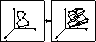
\includegraphics[width=10cm]{ilustrace/Il-2-3}
		\caption{Ilustrace vytváření trojrozměrného tělesa z oříznuté plochy.$x$,$y$,$z$ - osy světového souřadného systému, $A$ - oříznutá plocha,$v$ - vektor posunutí, $B$ - oříznutá plocha $A$ posunutá o vektor $v$.}
		\label{fig:10-1}
	\end{center}
\end{figure}

\subsection{Získání vektoru posunutí}
\label{vektorPosunu}
Jako vektor posunutí může být zvolena normála plochy, nebo třeba vektor odpovídající směru kamery. Každé z těchto řešení by přinášelo problém. 
\paragraph{}
Při použití normály by byl problém ten, že rovina získaná pomocí ransac algoritmu je pokaždé trochu jiná\footnote{Čím více jsou body použité na vytvoření roviny v jedné rovině, tím menší budou změny mezi plochami získanými při jednotlivých generacích.} tudíž vytažení objemu z plochy ve směru normály by při každé aktualizaci scény dávalo jiné výsledky.
\paragraph{}
Při použití směru kamery ale nastává jiný problém. Je velmi pravděpodobné, že uživatel bude chtít vytáhnout objem ve směru kolmém k základní ploše, nebo ve směru, který se ke kolmému směru blíží. V tomto případě by bylo potřeba použít fotografii, ve které budou vidět pouze podstavy výsledného tělesa a nebudou vidět boční stěny. (stěna by byla rovnoběžná se směrem kamery) a uživatel by v tu chvíli neměl žádné informace o oné stěně.To je ale problém, neboť uživatel bude muset měnit pohledy, aby viděl, jak přesně získané těleso pasuje na rekonstruovaný objekt. 
\paragraph{}
Třetí možnost by byla použít normálu ve chvíli prvního použití tohoto nástroje a neměnit ji při každé změně roviny plochy. V tomto případě je problém ten, že uživatel může na začátku omylem zadat plochu tak, že nebude vůbec odpovídat stěně, kterou má reprezentovat\footnote{Uživatel může zadat pro segmentaci body i z jiných stěn, nebo nezadá dost bodů. V tom případě bude mít stěna s nějvětší pravděpodobností jiné natočení i jinou pozici}. Z této plochy vytvoří trojrozměrné těleso.  Později si svou chybu uvědomí a nastaví plochu do správné roviny. Vektor posunutí bude stále nastaven na hodnotu normály ve chvíli, kdy nástroj použil. Proto bude potřeba dovolit uživateli změnit vektor posunutí a nastavit ho na hodnotu normály plochy v dané chvíli. S možností nastavit vektor na aktuální hodnotu normály plochy je toto řešení nejvýhodnější z výše zmíněných.
\paragraph{}
Dalším problémem je fakt, že ne vždy jsou směr pohledu kamery, nebo normála tím pravým. Proto by bylo třeba uživateli dovolit změnit směr tohoto vektoru, který bude použit pro vytažení objemu z plochy.

\subsection{Zobrazení v editoru fotografie}
\label{zobrazeniExtrude}
Pro práci s tímto nástrojem bude uživatel potřebovat nějakou zpětnou vazbu. Takovou, která by mu pomohla s nastavením správné délky a směru vektoru, o který se mají body posunout. Mohly by být uživateli zobrazeny všechny body těles, ne pouze body z původních ploch. Toto by ale mohlo být pro uživatele velmi matoucí, protože by ve scéně přibylo značné množství bodů. Proto by bylo vhodné zobrazit jen menší množství bodů. Například jen body patřící právě vybrané ploše. Také bude nezbytné odlišit body zadané do zobrazené fotografie, body zadané v jiné fotografii a promítnuté do této fotografie a také body, na které byl aplikován vektor posunutí, a pak byly promítnuty do fotografie.

\section{Texturování trojrozměrného tělesa}
Dále bude třeba vyřešit, jak spojit toto těleso s texturou, která byla aplikována na původní plochu. 

\subsection{Účel tohoto nástroje}
\label{teturovaniTelesa}
Tento nástroj je určen především k tomu, aby byl člověk schopen dosáhnout konkrétního tvaru, i když pro jeho rekonstrukci není dostatek dat, nebo tvaru, který neodpovídá jedné rovině. Toto by mohlo být využito například pro římsy, nebo jiné útvary, které mají po celé své délce stejný tvar. Další možností aplikace by byla například tašková střecha.
\paragraph{}
Takovéto útvary, například stěny s římsou, by byly nejdříve vytvořeny jako plochy v rovině kolmé k té, ve které se budou nacházet. Tím vznikne podstava budoucího trojrozměrného tělesa. Poté se z plochy vytvoří trojrozměrné těleso. Boční stěny tohoto tělesa budou reprezentovat danou stěnu s římsou. Následně uživatel bude pravděpodobně chtít toto těleso využít jako obyčejnou plochu a promítnout na ní texturu. To znamená, že uživatel vlastně použije pouze některé z bočních stěn tělesa. V tomto případě bude pro uživatele nejvhodnější promítnout texturu z pohledu kolmého na onu rekonstruovanou stěnu stejně tak, jako při promítání na obyčejnou plochu.
\paragraph{}
Takto bychom promítli všechny body tělesa do fotografie, pomocí které se texturuje. Problém může nastat v případě, že se uhel mezi normálou texturované stěny a vektorem pohledu kamery blíží k $90^{\circ}$. To by způsobilo mapování celé stěny na malé množství pixelů\footnote{Toto malé množství pixelů by bylo roztaženo po celé stěně a tak by na ní vznikly barevné šmouhy.}. Dále by mohl nastat problém při vytváření složitých těles. Čím složitější těleso by uživatel vytvářel, tím hůře by textura seděla.
\paragraph{}
Pokud by uživatel chtěl správně otexturovat všechny strany tělesa, bylo by vyžadováno využití nějakého obalového tělesa, přes které by se textura mapovala, nebo by uživatel musel mapovat texturu na každou stěnu tělesa zvlášť. Toto by uživateli značně komplikovalo jeho práci a ztrácela by se hlavní myšlenka programu. To, aby byl co nejjednodušší na použití uživatelem.
\paragraph{}
Zároveň by bylo nezbytné pro texturu použít více než jen jednu fotografii, neboť by chyběly všechny strany tělesa, které jsou na fotografii odvráceny. Toto by uživateli značně komplikovalo texturování i poměrně jednoduchého tělesa. 
\paragraph{}
Vzhledem k tomu, že nástroj má být jednoduchý a efektivní a implementace tohoto nástroje není mým úkolem, použiji první možnost. Body tělesa budou promítnuty do jedné fotografie a z těchto průmětů budou vypočítány texturovací souřadnice.

%
%
%
\chapter{Návrh}
V této části popíši návrh řešení problémů zmíněných v předchozích kapitolách (\ref{analyzaStart} - \ref{analyzaEnd}). 

\section{Importní modul pro VisualSFM}
\label{navrhStart}

%\subsection{Proces načtení}
Načtení dat do programu se provádí volbou Import Bundler v hlavním okně programu. Na tento element je posluchačem navázána obslužná funkce. Obslužná funkce nechá uživatele vybrat adresář, ze kterého chce scénu načíst, a cestu k tomuto adresáři použije spolu s konstantami k vytvoření cest k jednotlivým souborům, které se budou načítat. Poté je vytvořena instance třídy BundlerLoader, které jsou předány tyto cesty, odkud načítat scénu a metodou load je scéna načtena a následně je uložena do statických proměnných třídy MDI\_app\_state.  
Jelikož se data získaná z obou programů vlastně liší pouze adresářovou strukturou a názvy souborů, bude stačit použít metodu pro načítání dat získaných Bundlerem a pouze nahradit konstanty, které jsou využívány při vytváření správných cest.

\section{Nástroj pro vytváření hranic ploch}

\subsection{Zadávání hranice}
\label{cycle}
Hranici plochy bude uživatel zadávat do editoru fotografie. To znamená, že bude nezbytné upravit třídu MDI\_editor\_v1.
\paragraph{} 
V aktuálním stavu programu je při zvolení plochy z palety ploch automaticky aktivován nástroj pro kreslení do fotografie. Tímto nástrojem uživatel zadává data pro segmentaci fotografie. Jak už jsem dříve zmínil, tento nástroj bude nezbytné deaktivovat při zadávání bodů a následně i při úpravě bodů. Proto je nezbytné přidat možnost pro uživatele - přepínat mezi jednotlivými nástroji. 
\paragraph{}
V jednu chvíli tedy bude moci být aktivní pouze jeden nástroj. Pro výběr jednoho prvku z n nejlépe odpovídá RadioButton, kde jediný vybraný prvek bude odpovídat právě vybranému nástroji. Další možností by bylo využít tlačítko k cyklickému přepínání mezi nástroji.
\paragraph{}
Výhodou první možnosti je například rychlá možnost přepínání, pokud má člověk více stavů. Nevýhodou první možnosti je lineárně rostoucí velikost s přibývajícím počtem nástrojů. Výhody druhé možnosti jsou konstantní velikost. Na druhou stranu čas vybrání správného nástroje roste s přibývajícím množstvím nástrojů.
\paragraph{}
V tomto případě je velikost GUI poměrně omezená, neboť zvětšování panelu nástrojů by vedlo k zmenšování pracovní plochy editoru. Zároveň budou k dispozici pouze tři nástroje, takže cyklické procházení nástrojů nebude uživatele příliš zdržovat. Kromě toho se dá předpokládat, že uživatel nejdříve zadá data pro segmentaci fotografií, poté zadá hranice jednotlivých ploch a nakonec zpřesní pozici vrcholů těchto ploch, tudíž nebude muset příliš přepínat mezi nástroji. Z důvodu ušetření prostoru tedy volím cyklické procházení nástrojů.

\subsection{Nástroje}
Události myši, které editor registruje, jsou "click", "drag" a "release". V každé z obslužných metod pro tyto události je napevno připojena akce, která bude vykonána. Proto bude třeba přidat do obslužných metod switch, který bude pomocí vybraného nástroje rozhodovat, která část kódu bude zavolána. Toto umožní v budoucnosti relativně snadné přidávání dalších nástrojů, když každý nástroj bude od ostatních kompletně oddělen. Kompletní oddělení nástrojů od sebe sice způsobí vznik duplicitního kódu\footnote{Jednou z těchto duplicit může být například transformace pozice kurzoru vůči oknu do pozice vůči fotografii.}, ale těchto částí bude pouze malé množství.

\subsection{Zpracování události}
Při kliknutí do fotografie je vygenerována událost, se kterou je zavolána obslužná metoda. Z události získáme pozici kurzoru v době kliknutí.Pozice kurzoru je vůči oknu editoru. Tento bod musí být nejdříve zpracován, aby mohl být použit k promítnutí do roviny. Fotografie v editoru totiž může být zvětšená/zmenšená, otočena o násobky $90^{\circ}$ a posunutá v osách $x$ a $y$. Tyto transformace jsou uloženy jako instance třídy AffineTransform. Tato transformace se využívá pro správné vykreslení objektů do fotografie. Editor si zároveň uchovává i inverzní transformaci k této transformaci pro případ zadávání dat. Tudíž aplikujeme inverzní transformaci na zadaný bod. Nyní ještě zbývá převrátit osu y a bod je připraven k uložení.

\subsection{Uložení hranice}
Jak vyplývá z předchozích částí ( \ref{hraniceUlozeni} a \ref{hraniceViceBodu} ), hranice by měla být uložena jako uspořádaná množina hraničních bodů. Každý z hraničních bodů bude uchovávat množinu 2D bodů, kde ke každému z těchto bodů bude přiřazena právě jedna kamera (kamera odpovídající fotografii, ve které byl bod zadán). Tato množina bodů a kamer nemá omezenou velikost, ale musí obsahovat alespoň jednu dvojici kamera-bod. Dvojice bude možné do množiny přidávat i odebírat, ale každá kamera může být v množině nejvýše jedenkrát. Pro vykreslování bodů do fotografií bude nezbytné, aby bylo možné zjistit, jestli pro danou kameru už v množině nějaká dvojice tuto kameru obsahující a pokud ano, tak získat tento bod. Dále pro výpočet průměru průmětů bodů bude třeba moci iterovat přes všechny dvojice. Dle mého názoru tomuto nejlépe odpovídá HashMapa, kde kamera bude klíčem a 2D bod hodnotou. Díky HashMapě bude rychlé zjišťování, zda je už daný klíč (kamera) použit, i bez nutnosti iterovat přes všechny prvky množiny. 
\paragraph{}
Jak bylo dříve zmíněno (\ref{hraniceUlozeni}), tato množina hraničních bodů by měla být uložena v objektu plochy. Objekt plochy je třídy CSG\_Plane a ke správné instanci je možné se dostat přes právě používanou scénu uloženou v MDI\_app\_state.

\subsection{Aplikace hranice}
Dalším krokem je promítnutí hranice na plochu. Jak už jsem výše zmínil, plocha je reprezentována množinou bodů a rovinou. Rovina je reprezentována čtyřmi parametry $a$, $b$, $c$, $d$, které odpovídají parametrům obecné rovnice roviny, tj. $a*x+b*y+c*z+d=0$.
\paragraph{}
Také jsme schopni promítnout bod z fotografie pomocí její kamery. K tomu ale bude nezbytné transformovat body hranice, neboť byly zadány v jiné souřadné soustavě.

\subsection{Transformace bodu a kamery}
\label{promitnuti}
Body hranice byly zadány vůči oknu editoru, kde počátek souřadné soustavy je v levém horním rohu, kladná osa $X$ směřuje vpravo a kladná osa $Y$ směřuje dolu. Nejdříve bude nezbytné transformovat 2D bod hranice tak, aby jeho souřadnice byly vůči středu fotografie. Toho dosáhneme posunutím bodu o polovinu šířky fotografie po ose $X$ a o polovinu výšky fotografie v ose $Y$. Dále bude třeba obrátit osu $Y$ tak, aby její kladná část směřovala vzhůru, k čemuž nám postačí změnit znaménko $y$ souřadnice bodu. Tyto transformace bude vhodné použít už při ukládání bodu, který uživatel zadal, neboť promítání se bude vykonávat po každé provedené změně ve scéně a bylo by zbytečné pokaždé provádět tuto transformaci. To znamená, že všechny hraniční body budou mít souřadnice vůči středu fotografie, do které byly zadány.
\paragraph{}
Nyní, abychom mohli vytvořit promítací přímku $p$, budeme potřebovat z bodu hranice, který si označíme jako bod $H$, vytvořit trojrozměrný bod, který použijeme při promítání. Tento bod si označme jako bod $P$. Jak už bylo zmíněno dříve \ref{modelKamery}, body, které budou použity pro promítání, jsou v obrazové rovině $b$. Tato rovina $b$ je kolmá na osu $Z$ v souřadné soustavě kamery a je od středu kamery posunuta o vzdálenost $f$ v záporném směru osy $Z$. Vzdálenost $f$, tedy ohnisková vzdálenost kamery, tedy bude určovat souřadnici $z$ bodu $P$, neboť pozice bodu v obrazové rovině nemůže ovlivnit souřadnici $z$\footnote{Obrazová rovina je rovnoběžná s rovinou $XY$ v soustavě kamery.}. Nyní je potřeba získat hodnoty souřadnic $x$ a $y$ bodu $P$. Ty snadno získáme z bodu $H$. Souřadnice tohoto bodu ani nebude třeba nijak dále upravovat, neboť ohnisková vzdálenost je ve stejných jednotkách jako souřadnice bodu ve fotografii. To znamená, že z bodu $H$ se souřadnicemi $(x, y)$ vytvoříme bod $P$ tak, že bodu $H$ přidáme souřadnici $z$. Souřadnice bodu $P$ tedy budou $(x, y, -f)$. Promítací přímku získáme tak, že proložíme přímku bodem $(0, 0, 0)$, který odpovídá středu kamery, a bodem $P$.
\paragraph{}
V předchozím odstavci jsme vše řešili v souřadné soustavě kamery, ale pro další použití budeme potřebovat promítací přímku ve světových souřadnicích. Jelikož je přímka určena dvěma body, stačí transformovat oba řídící body přímky, tj. střed kamery a promítací bod $P$, pomocí transformací kamery a následně jimi proložit přímku. Když už získáme tuto přímku, snadno dopočítáme její průsečík s rovinou.

\subsection{Nalezení 3D bodu reprezentujícího hraniční bod}
\label{hraniceJedenBod}
Máme tedy rovinu a hranici plochy. Hranice každé plochy je uspořádaná množina hraničních bodů, kde každý z těchto objektů udržuje množinu dvojic kamera-bod. Pokud tedy pro každou dvojici kamera-bod promítneme onen bod onou kamerou do roviny plochy, získáme 3D bod. Když už máme pro daný hraniční bod pro všechny dvojice kamera-bod získány 3D body, bude třeba získat jeden bod, který bude tuto množinu 3D bodů reprezentovat. Jako tento jediný bod jsem se rozhodl použít těžiště množiny bodů\footnote{Rozdíly v pozici těchto bodů by v rámci scény měly být minimální, pokud uživatel zadává dobrá data. Čím horší data uživatel bude zadávat, tím nepřesnější výsledky bude program dávat.}. Tímto způsobem získáme pro každý hraniční bod v hranici jeden trojrozměrný bod. Tento bod můžeme použít pro vytvoření finální geometrie. 

\subsection{Vytváření geometrie}
\label{volbaMetody}
Momentálně je geometrie plochy vytvářena ve statické metodě findBestVisualization4 třídy Plane3Dutils. Tato metoda je volána v metodě reconstructPlane třídy SegmentationWrapper, kde je metodě findBestVisualization4 předána rovina, body, ořezávací přímky\footnote{Přímka reprezentující průsečík dvou ploch, které se mají navzájem ořezávat.} a index plochy, která je vytvářena. Výsledek findBestVisualization4 je uložen do odpovídající instance třídy CSG\_Plane. 
\paragraph{}
Proto bude třeba vytvořit metodu, která promítne hranici do roviny a použije získané body k vytvoření geometrie. Momentálně je k vytvoření geometrie používán objekt GeometryInfo, který dovoluje vytváření nekonvexních těles zadáním jejich hranice. Z tohoto objektu je vytvořen objekt GeometryArray, který reprezentuje geometrii výsledné plochy a je možné z něj vytvořit objekt zobrazitelný ve scéně.
\paragraph{}
Která z těchto metod bude v reconstructPlane zavolána pro vytvoření geometrie, se zvolí na základě toho, zda je zadáno dostatečné množství bodů do hranice, tj. alespoň $3$ body. 

\subsection{Zobrazení hranice v editoru}
Celá hranice plochy je tvořena hraničními body. Každý bod hranice je zadán v n různých fotografiích a každý z těchto bodů hranice bude třeba vykreslit ve fotografii zobrazené v editoru. Pokud je hraniční bod zadán v zobrazené fotografii, můžeme ho použít. Pokud zadán nebyl, budeme muset vzít hraniční bod a promítnout ho do zobrazené fotografie.  To znamená, že budeme potřebovat 3D reprezentaci hraničního bodu (viz. \ref{hraniceJedenBod}). K promítnutí 3D reprezentace hraničního bodu do fotografie bude možné použít obdobný princip, jakým byl bod promítnut z fotografie do roviny (\ref{promitnuti}).

\subsection{Promítnutí do fotografie}
\label{promitaniDoFotografie}
Máme 3D bod $B$, který budeme promítat, a máme i kameru fotografie, do které ho budeme promítat. Pro toto promítání můžeme opět využít upravený Pinhole Camera Model(viz. \ref{modelKamery}). Střed kamery $S$ získáme z objektu kamery. Paprsek získáme tak, že vytvoříme přímku procházející bodem $S$ a bodem $B$. Nyní bude třeba získat rovinu odpovídající obrazové rovině $b$. K tomu potřebujeme jeden bod v této rovině a normálu roviny. Pokud bychom měli bod, odpovídající průniku obrazové roviny $b$ a optické osy (osa $Z$ v souřadném systému kamery), budeme mít jak bod v oné rovině, tak dokážeme spočítat normálový vektor s pomocí středu kamery. Tento bod ovšem dokážeme získat a označíme si ho $O$.  Je to totiž bod $(0,0,-f)$ v souřadnicích kamery. To znamená, že stačí aplikovat transformace kamery a získáme světové souřadnice tohoto bodu $O$. Stejnou transformaci aplikujeme i na střed kamery $S$. Odečtením bodů $O$ a $S$ získáme normálu roviny, jako bod v rovině použijeme bod $O$. Takto můžeme vytvořit rovnici obrazové roviny $b$. Parametry $a$, $b$ a $c$ získáme z normály a $d$ vypočteme pomocí bodu $O$. Nyní vytvoříme přímku mezi promítaným bodem a středem kamery a najdeme průsečík s obrazovou rovinou $b$. Tento průsečík si označíme, jako bod $P$. Na bod $P$ aplikujeme inverzní transformaci k transformaci kamery a tím získáme bod $P'$. Takto získáme souřadnice bodu $P$ v souřadném systému kamery. Bod $P'$ bude mít souřadnici z rovnu $-f$ a souřadnice $x$,$y$ budou pozice promítnutého bodu vůči středu fotografie.
\paragraph{}
Výše zmíněný způsob promítání není jediný. Celé promítání je možné reprezentovat jako maticové násobení.

\subsection{Promítnutí do fotografie (maticově)}
\label{promitaniMat}
Z bodu $B$, což je nějaký 3D bod ve světových souřadnicích, potřebujeme získat 2D bod $P'$ v souřadnicích fotografie. Pro tuto projekci je nezbytné použít homogenní souřadnice(vice v kapitole \ref{homog}) a výsledná projekce lze vyjádřit následující rovnicí.

$
\begin{bmatrix}
	Px \\
	Py \\
	1
\end{bmatrix}
=
C
\times
\begin{bmatrix}
Bx \\
By \\
Bz \\
1
\end{bmatrix}
$

$Px$ a $Py$ jsou souřadnice promítnutého bodu (bod $P'$) vůči středu fotografie, $Bx$,$By$,$Bz$ jsou souřadnice promítaného bodu (bod $B$) vůči světovému souřadném systému a $C$ je promítací matice $3\times4$. Matici $C$ je možné rozdělit na matici $I$ a $E$, kde matici $I$ budeme označovat jako vnitřní parametry kamery\footnote{z anglického "Intrinsic parameters/matrix"} a matici $E$ budeme označovat jako vnější parametry kamery\footnote{z anglického "Extrinsic parameters/matrix"}. Matice $I$ má rozměry $3\times4$, matice $E$ má rozměry $4\times4$ a platí, že $C = I \times E$.
\paragraph{}
Jelikož v našem případě nedochází ke zkosení fotografie, pixely jsou čtvercové a optická osa prochází středem fotografie, můžeme matici $I$ zjednodušit do následujícího tvaru.
 
 $$
 I
 =
 \begin{bmatrix}
 	f & 0 & 0 & 0 \\
 	0 & f & 0 & 0 \\
 	0 & 0 & 1 & 0
 \end{bmatrix}
 $$
 V tomto pípadě parametr $f$ je ohnisková vzdálenost, který je vyjádřeana v pixelech. Matici $E$ můžeme vyjádřit jako součin dvou matic $T$ a $R$, kde obě matice jsou rozměrů $4\times4$. V tomto případě matice $T$ označuje translaci\footnote{Parametry $tx$, $ty$ a $tz$ označují souřadnice počátku světové souřadné soustavy v kamerových souřadnicích.  Více informací o translaci v Moderní počítačová grafika\cite{Zara}, část E, kapitola 21.3.1} a matice $R$ znamená rotaci\footnote{Parametry $r_{i,j}$ reprezentují rotační matici. Více informací o rotaci v Moderní počítačová grafika\cite{Zara}, část E, kapitola 21.3.2}.
 $$
 E = T \times R
 $$
 
 $$
 E
 =
  \begin{bmatrix}
  1 & 0 & 0 & tx\\
  0 & 1 & 0 & ty\\
  0 & 0 & 1 & tz\\
  0 & 0 & 0 & 1
  \end{bmatrix}
  \times
  \begin{bmatrix}
  r_{1,1} & r_{1,2} & r_{1,3} & 0\\
  r_{2,1} & r_{2,2} & r_{2,3} & 0\\
  r_{3,1} & r_{3,2} & r_{3,3} & 0\\
  0 & 0 & 0 & 1
  \end{bmatrix}
 $$
 Důležité je zmínit, že matice $T$ a $R$, tudíž i matice $E$, nereprezentují transformaci kamery vůči světové souřadné soustavě, ale transformaci světového souřadného systému vůči kameře. To znamená, že bod ve smětových souřadnicích vynásobený zleva maticí E bude transformován do systému kamery. Následně se takto transformovaný bod zleva vynásobí maticí I a tím získáme souřadnice promítnutého bodu ve fotografii.
 
\subsection{Homogenní souřadnice}
\label{homog}
Homogenní souřadnice\cite{Zara} jsou způsob reprezentace 2D a 3D bodů. Máme-li bod $A$, kteý je v kartézských souřadnicích vyjádřen jako $A = (Ax ,Ay)$, bude tento bod vyjádřen v homogenních souřadnicích jako $(x, y, z)$ přičemž platí, že $Ax = \frac{x}{z},Ay = \frac{y}{z}$ a zároveň platí, že $z \neq 0$\footnote{Pokud dvojrozměrnému bodu v kartézských souřadnicích $A = (Ax, Ay)$ odpovídá bod v homogenních souřadnicích $A' = (A'x, A'y, A'z)$, potom platí, že $A = (\frac{A'x}{A'z},\frac{A'y}{A'z})$ a $A' = (kAx, kAy, k), k\in\mathbb{R}-{0}$}. 
\paragraph{}
Obdobně je tomu i u trojrozměrných bodů, které jsou rozšířeny o složku $w$. Potom z trojrozměrného bodu v kartézských souřadnicích B = (Bx, By, Bz) bude v homogenních souřadnicích bod B = (x, y, z, w) přičemž bude platit že $Bx = \frac{x}{w},By = \frac{y}{w},Bz = \frac{z}{w}$ a $w \neq 0$.
\paragraph{}
Tato reprezentace je využívána především kvůli tomu, že homogenní souřadnice nám dovolují reprezentovat posunutí maticovým násobením (to v kartézských souřadnicích není možné, zde je nutné použít sčítání). Druhou výhodou, kterou nám homogenní souřadnice přinášejí je to, že bod v homogenních souřadnicích vlastně reprezentuje přímku procházející středem souřadného systému v o jednu dimenzi vyšším prostoru\footnote{Toho je využito přávě při promítání do fotografie při použití matic (viz. \ref{promitaniMat}).}) \footnote{Více informací o homogenních souřadnicích v Moderní počítačová grafika\cite{Zara}, část E, kapitola 21.1}.  
 
 
\begin{figure}[]
	\begin{center}
		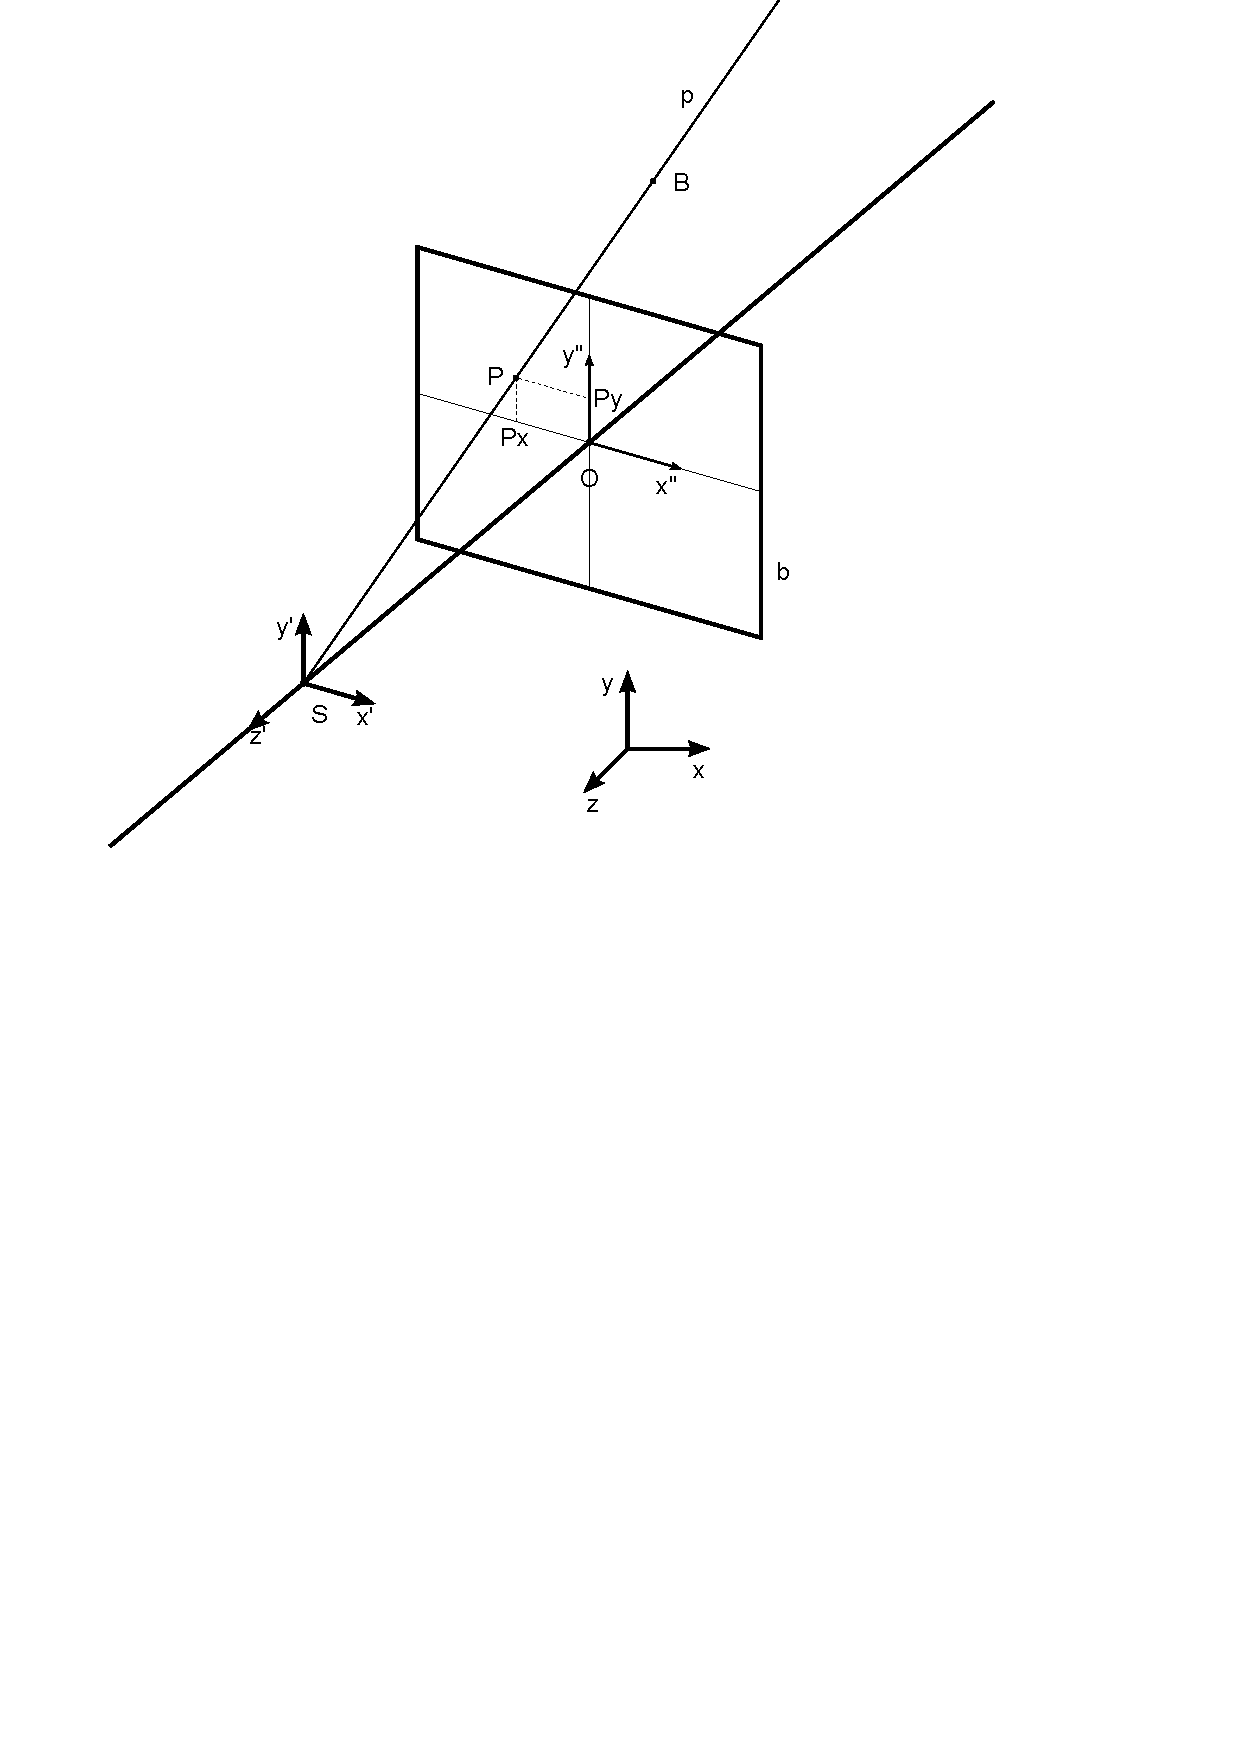
\includegraphics[width=10cm]{ilustrace/Il-6-1}
		\caption{Ilustrace promítání 3D bodu do fotografie. $x$,$y$,$z$ - osy světového souřadného systému, $x'$,$y'$,$z'$ - osy souřadného systému kamery, $x''$,$y''$,$z''$ - osy souřadného systému fotografie, $b$ - obrazová rovina, $B$ - promítaný bod, $S$ - střed kamery, $O$ - průsečík optické osy s rovinou $b$ a také počátek souřadného systému fotografie, $p$ - promítací paprsek procházející bodem $B$ a středem kamery $S$, $P$ - průsečík promítacího paprsku $p$ a roviny $b$, $Px$,$Py$ - souřadnice bodu P v souřadné soustavě fotografie.}
		\label{fig:6-1}
	\end{center}
\end{figure}

\clearpage

\subsection{Transformace bodu pro zobrazení v editoru}
Nyní vytvoříme 2D bod z transformovaného bodu $P$ zahozením složky $z$ a transformujeme ho do souřadnic fotografie tak, že posuneme osy $x$ a $y$ a osu $y$ převrátíme. Nakonec aplikujeme transformaci fotografie. Takto získáme přesnou pozici bodu v okně editoru fotografie.


\begin{figure}[]
	\begin{center}
		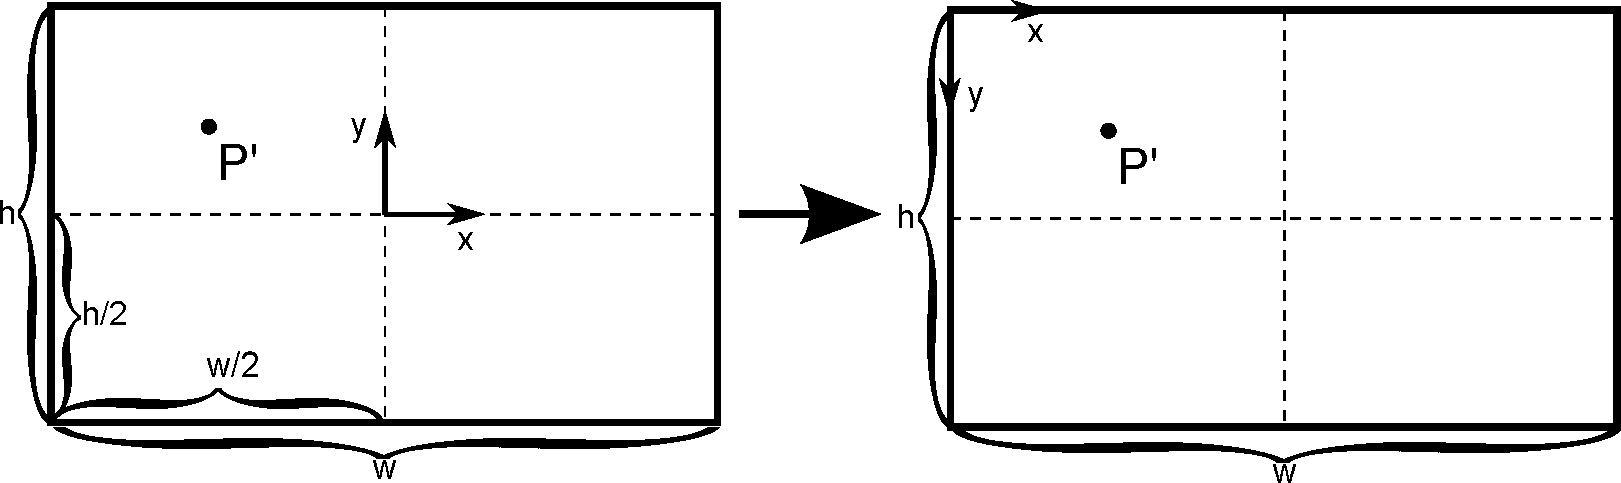
\includegraphics[width=13cm]{ilustrace/Il-7-1}
		\caption{Ilustrace transformace souřadnic bodu. $P'$ - bod promítnutý do fotografie, $h$ - výška fotografie, $w$ - šířka fotografie}
		\label{fig:7-1}
	\end{center}
\end{figure}

\subsection{Barva hranice}
Pro určení barvy plochy je použit barevný model HSB. Pokud uvažujeme, že barevný tón (hue), sytost (saturation) i jas (brightness) nabývají hodnot z intervalu $<0,1>$, tak pro rovinu s indexem i je barevný tón nastaven na hodnotu $(i*40/255) mod (1)$ a sytost i jas jsou nastaveny na maximum. 

\subsection{Způsob zobrazení hranice a jejich bodů}
Nejvhodnější bude zobrazit body hranice a spojnice mezi nimi. Spojnice reprezentované úsečkami budou spojovat vždy dva sousední body. Aby uživatel měl nějaké informace o počátku a konci hranice, první bod s posledním nebude spojen. Toto umožní uživateli poznat, mezi které dva body bude přidán další bod.

\subsection{Způsob vykreslování v editoru}
\label{vykresleni}
Hlavní problém je v tom, jakým způsobem body a hranice vykreslit. V editoru fotografií se vše vykresluje po jednotlivých vrstvách. Nejspodnější vrstva je fotografie. Na ní je vykreslena poloprůhledná vrstva dávající uživateli informace o segmentaci fotografie. Každý segment odpovídající jedné ploše má barvu odpovídající této ploše. Přes tuto vrstvu se zobrazují obrazce nakreslené uživatelem, když zadával data pro segmentaci.
\paragraph{}
Body a hranice bude vhodné vykreslovat v úplně nejvyšší vrstvě, neboť jsou to nejmenší objekty a neměly by být překryty. Problém zmíněný výše je ale ten, jak zvolit barvy, aby body byly vidět.
\paragraph{}
Například máme plochu, které odpovídá žlutá barva. Hranici této plochy budeme pravděpodobně zadávat na oblasti, která odpovídá této ploše. To znamená, že oblast bude ve fotografii po segmentaci překryta poloprůhlednou žlutou vrstvou. Následně se může stát, že v místě bodu bude obrazec nakreslený uživatelem, který bude žlutý a neprůhledný. Pokud bychom bod vykreslili žlutou barvou, buď nebude vidět vůbec, a nebo ho bude díky poloprůhledné vrstvě špatně vidět. 

\subsection{Řešení viditelnosti}
Logické řešení by bylo použít inverzní barvu. Ta by byla kontrastní k barvě plochy a bod by byl výborně vidět. Uživatel ale nemusí znát ke každé barvě její inverzní barvu a bylo by to pro něj matoucí. Zároveň by se mohlo stát, že inverzní barva bude odpovídat barvě jiné plochy a kdyby uživatel zadal bod do oblasti této plochy, opět by nebyl vidět.
\paragraph{}
Proto nejvhodnější bude použít bod v barvě odpovídající ploše a dát mu kontrastní okraj, například z inverzní barvy. Případ, že by inverzní barva byla shodná s původní, nastat nemůže. To by vyžadovalo, aby sytost původní barvy byla minimální a jas měl hodnotu $0,5$. Jelikož sytost i jas původní barvy jsou vždy $1$, tj. maximum, tento problém nenastane.  Dále bychom mohli použít okraj v odstínech šedi, neboť žádné z rovin nebudou tyto barvy odpovídat.
\paragraph{}
Dále musíme rozlišit, zda byl zobrazovaný bod zadán v zobrazené fotografii, nebo zda je do ní pouze promítán. Zadaný bod tedy bude vykreslen s okrajem v inverzní barvě a promítaný bod s šedivým okrajem. Takto uživatel snadno pozná, který z bodů byl v zobrazené fotografii zadán a který ne. 

\section{Zpřesňování hranice plochy}
Do editoru fotografie bude nutné přidat další nástroj. Při používání tohoto nástroje musí být vypnuty nástroje pro kreslení do fotografie i pro zadávání bodů. Bude tedy přidán do cyklického přepínání mezi nástroji.

\subsection{Výběr bodu}
Nejprve bude třeba vybrat bod hranice, který se bude upravovat. Podle dřívější kapitoly bod bude vybrán kliknutím poblíž něj. Toto vybírání bodů se bude provádět pouze mezi body, které patří do plochy, která je momentálně vybrána. To sníží počet bodů, mezi kterými se bude vybírat, a lépe se budou vybírat body, které jsou velmi blízko jiných bodů.
\subsection{Změna pozice bodu}
V metodě obsluhující událost "click" tedy bude potřeba promítnout všechny body dané plochy do fotografie, která je zobrazena v editoru. Následně se nalezne nejbližší bod k pozici kurzoru v době kliknutí a tento bod se nastaví jako vybraný.  
\paragraph{}
Na vybraný bod bude vhodné uchovávat referenci přímo v editoru fotografie.
\paragraph{}
Nyní pokud uživatel stiskne libovolné tlačítko myši a pohne s myší, vybraný bod by se měl nastavit na pozici kurzoru. To znamená, že bude třeba upravit metodu obsluhující událost "drag". Zde bude třeba zjistit, zda vybraný bod hranice už byl v této fotografii zadán. Pokud ano, nastavit pozici bodu tohoto bodu v této fotografii na pozici kurzoru a pokud ne, přidat hraničnímu bodu pro tuto fotografii bod odpovídající pozici kurzoru. Tato událost je volána při změně pozice kurzoru, proto je volána mnohokrát během přemisťování bodu.  I když je v tuto chvíli potřeba překreslovat okno editoru, aby uživatel měl přehled o aktuální pozici bodu, není vhodné pokaždé upravovat 3D scénu, jejíž vytváření je náročnější. Bude vhodné upravit ještě metodu obsluhující událost "release", aby byla zavolána aktualizace 3D scény. Takto se 3D scéna znovu vytvoří, až uživatel pustí tažený bod.

\subsection{Nástroj pro změnu stavu bodu}
\label{fixaceBodu}
Dále bude třeba vytvořit nástroj, který umožní odebrání  vybraného hraničního bodu z fotografie, pokud v ní byl zadán, nebo přidání bodu a fotografie do vybraného hraničního bodu, pokud do fotografie zadán nebyl. Pro toto bude vhodné přidat do editoru tlačítko, které umožní změnu těchto dvou stavů. V případě, že vybraný hraniční bod nebyl v této fotografii zadán, přidá se mu dvojice kamera-bod, kde kamera bude odpovídat zobrazené fotografii a bod bude průmět vybraného bodu do zobrazené fotografie. Pokud byl bod zadán v této fotografii a byl zadán i v jiných fotografiích, bude vybraný hraniční bod odstraněn ze zobrazené fotografie. Pokud je vybraný bod zadán pouze v této fotografii, nemůže být odebrán, protože by vybraný bod nebyl zadán v žádné fotografii a nebylo by možné jej promítnout do roviny plochy. 

\subsection{Nepřesnost}
Jak už jsem dříve zmínil, když je jeden bod zadán ve více fotografiích a výsledný 3D bod (dále jen průměrný bod) se vypočítává jako těžiště průmětů všech těchto bodů do roviny, začínají zde vznikat nepřesnosti. Přesněji řečeno pokud je v zobrazené fotografii zadán bod, průmět průměrného bodu se může zobrazit na úplně jiném místě, než bod zadaný uživatelem. Tuto nepřesnost je uživateli nezbytné nějak naznačit, aby věděl, že něco nezadal přesně, nebo že možná něco zadal chybně.
\paragraph{}
Problémem je jak uživatele informovat o nepřesnosti a její velikosti bez toho, aby bylo přes fotografii vykreslováno příliš mnoho informací. Kromě věcí zmíněných dříve (viz. \ref{vykresleni}), budou vykreslovány body a hranice, které uživatel zadal, a následně i body tělesa, pokud jsou některé z ploch rozšířeny o třetí rozměr \ref{zobrazeniExtrude}.
\paragraph{}
Zobrazením pozice bodu, kam se průměrný bod do fotografie promítne, by přidalo další bod do fotografie a nebylo by úplně jasné, ke kterému bodu patří\footnote{Průměrný bod může promítnout prakticky kdekoliv, pokud body jemu odpovídající byly v jiných fotografiích zadány na velmi odlišných místech.}, a především by to uživatele vedlo k tomu, aby přesunul daný bod do místa, kam se průměrný bod promítá. Tímto by snížil odchylku bodu ve fotografii od průmětu průměrného bodu, což ale nemusí problém řešit, neboť špatně umístěné mohou být body v jiných fotografiích, nebo může být chyba v rovině této plochy\footnote{rovina může mít málo bodů, nebo může obsahovat i body které patří jiné části scény}. 
\paragraph{}
Tato nepřesnost by šla vyjádřit například vykreslením kružnice kolem bodu, kde poloměr kružnice bude vzdálenost od průmětu průměrného bodu. Takto bude uživateli graficky znázorněno, jak moc se body od sebe liší. Ke kterému bodu daná kružnice patří, zjistí snadno, neboť onen bod je středem této kružnice.  Uživatel na první pohled pozná, zda je s některým z těchto bodů problém, protože veliká kružnice bude jen těžko přehlédnutelná. Také do fotografie nepřibude příliš mnoho dalších věcí. Především pokud budou kružnice zobrazeny pouze u vybrané plochy.

\section{Otexturování oříznuté plochy}

\subsection{Uložení textury}
Jelikož textura je jedna z vlastností ploch, měla by být uložena ve třídě plochu reprezentující. Touto třídou je CSG\_Plane.  

\subsection{Texturovací nástroj}
Bude třeba vytvořit nástroj v editoru fotografie. Jak bylo zmíněno dříve (\ref{texturovaniPlochy}), vhodným řešením bude tlačítko. Po jeho stisknutí se na vybranou plochu aplikuje textura z fotografie zobrazené v editoru. V metodě obsluhující událost stisknutí bude nezbytné vzít fotografii zobrazenou v editoru a pomocí ní texturu vytvořit. Jelikož je zde fotografie načtená, bylo by zbytečné ukládat pouze objekt třídy Image. Tento objekt sice fotografii reprezentuje, ale neuchovává ji načtenou, což znamená, že by bylo při použití nezbytné fotografii znovu načíst. Načtená fotografie je uložena v proměnné currentRaster (instance třídy BufferedImage). Takto jsme schopni pomocí instance třídy TextureLoader získat z dat uložených v currentRaster instanci třídy Texture, kterou budeme moci použít přímo při vytváření plochy. Takto získanou texturu poté uložíme do objektu odpovídajícímu ploše.

\subsection{Vytváření plochy a aplikace textury}
Objekt reprezentující plochu, který bude zobrazen ve 3D scéně, je vytvářen ve třídě CSG3D v metodě createPlane. V této metodě je využíván objekt GeometryArray\footnote{Tento objekt GeometryArray je vytvářen a ukládán do instance CSG\_Plane v metodě reconstructPlane, kde dochází ořezávání roviny pomocí hranice. viz. \ref{vytvareniPlochy}} odpovídající plochy a je tu i vytvářen materiál a celkový vzhled výsledné plochy. Zde bude třeba z používané instance CSG\_Plane vzít uloženou texturu a aplikovat ji. To se provede připojením objektu textury k instanci Appearance. Instance trídy Appearance je zde vytvářena a reprezentuje výsledný vzhled objektu.

\subsection{Texturovací souřadnice}
\label{texturovacíSouřadnice}
Každému 3D bodu použitému k vytvoření výsledné plochy bude nezbytné vypočítat texturovací souřadnice u a v tak, aby se správné vrcholy plochy mapovaly na správná místa v textuře. K tomu nám poslouží promítání 3D bodu do fotografie, které je využíváno při zobrazování bodů(viz. \ref{promitaniDoFotografie}). To znamená, že budeme kromě textury u objektu plochy uchovávat i informaci, ze které fotografie texturujeme, abychom měli přístup ke kameře odpovídající této fotografii. Díky této kameře budeme moci promítnout body hranice do fotografie a získat texturovací souřadnice. Takto získané souřadnice bude nezbytné přepočítat, neboť texturovací souřadnice u a v nabývají hodnot v intervalu $<0,1>$.  Promítnutím bodu do fotografie získáme 2D bod se souřadnicemi vůči středu fotografie (viz. obrázek \ref{fig:6-1}). Proto bude nezbytné k souřadnicím $x$ a $y$ bodu přičíst polovinu šířky, respektive výšky fotografie. Tím získáme souřadnice bodu vůči levému dolnímu rohu fotografie.  Následně vydělíme souřadnice $x$ a $y$ šířkou, respektive výškou fotografie, čímž ze souřadnic $x$ a $y$ získáme texturovací souřadnice $u$ a $v$ daného bodu. 

\begin{figure}[h]
	\begin{center}
		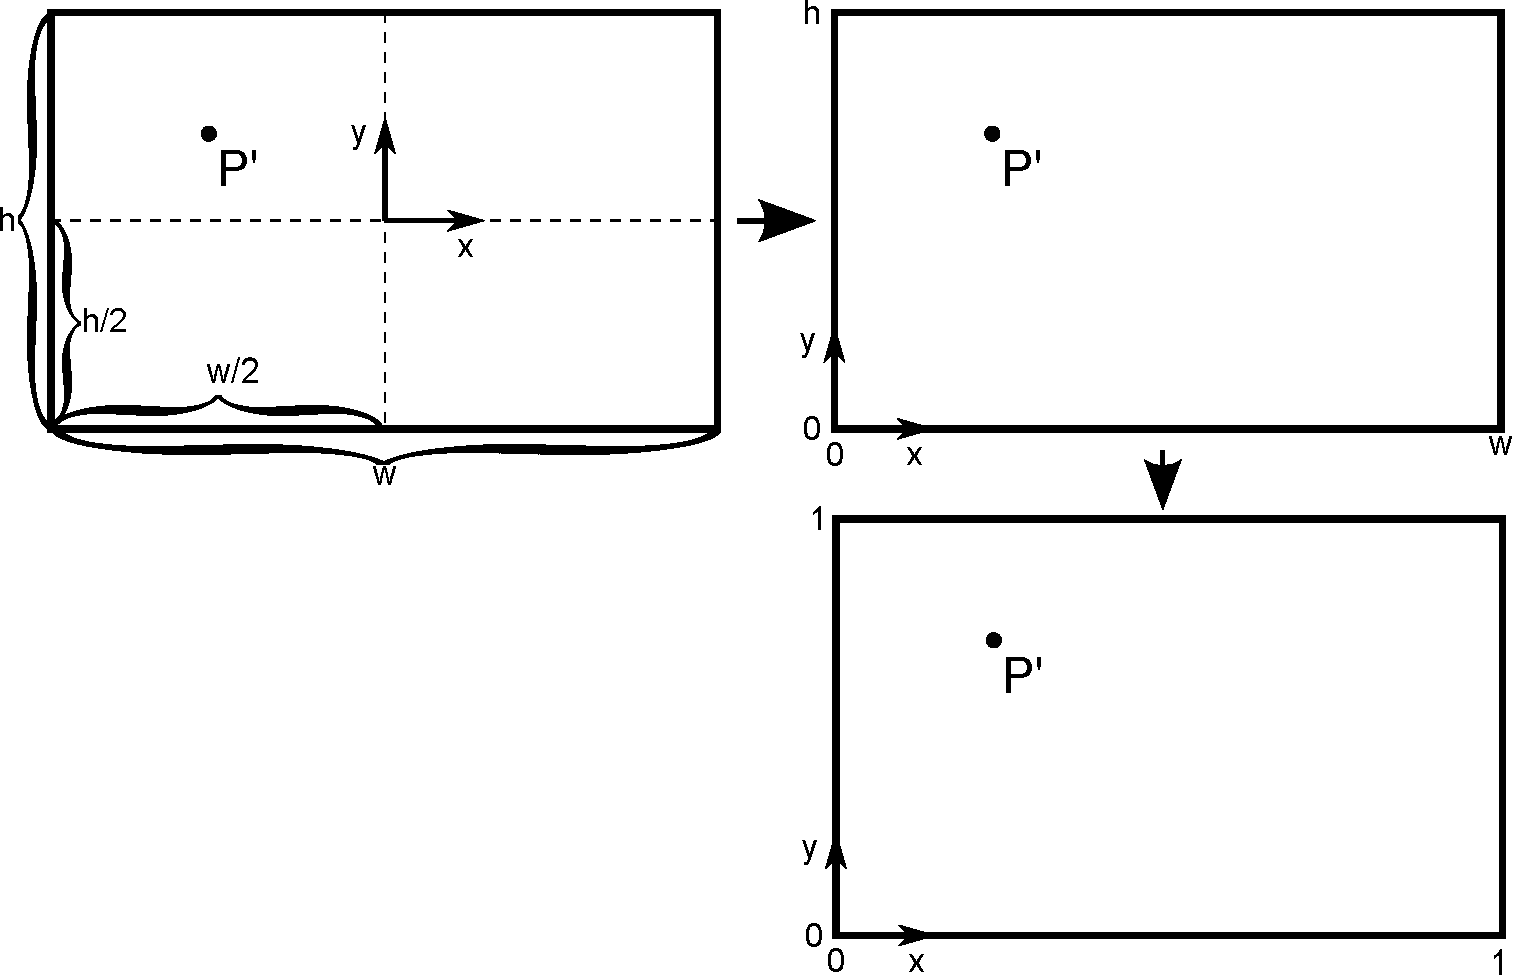
\includegraphics[width=13cm]{ilustrace/Il-8-1}
		\caption{Ilustrace transformace souřadnic bodu. $x$,$y$ - osy souřadného systému, který transformujeme, $P'$ - bod promítnutý do fotografie, $w$ - šířka fotografie, $h$ - výška fotografie.}
		\label{fig:8-1}
	\end{center}
\end{figure}

\subsection{Aplikace texturovacích souřadnic}
Texturovací souřadnice se zadávají ke každému bodu při vytváření geometrie plochy. Takže k metodě, která bude zajišťovat ořezávání plochy pomocí hranice, přidáme i tento výpočet texturovacích souřadnic.  Následně se vypočítané texturovací souřadnice uloží do objektu GeometryInfo.

\section{Vytvoření trojrozměrného tělesa z plochy}
\label{navrhEnd}
Jak bylo zmíněno dříve (viz. \ref{extrude}), při vytváření trojrozměrného tělesa se původní plocha stane podstavou tohoto tělesa, kopie podstavy posunutá o nějaký vektor bude druhou podstavou a tyto podstavy budou spojeny bočními stěnami. Dále (\ref{vektorPosunu}) jsme dospěli k tomu, že jako základ tohoto vektoru se použije normála plochy, ze které těleso vytváříme, a uživatel dále tento vektor upraví, pokud bude chtít. Úpravami je zde myšlena změna velikosti vektoru a také změna jeho směru.  

\subsection{Nástroj pro vytvoření tělesa}
Pro vytvoření tělesa z oříznuté plochy potřebujeme znát pouze informace o dané ploše. Konkrétně její normálový vektor. Nejvhodnější tedy bude přidat do GUI editoru tlačítko, po jehož stisknutí bude z plochy, která je vybrána v paletě ploch, vytvořeno trojrozměrné těleso. Normálu plochy použijeme jako vektor, kterým posuneme body druhé podstavy.
\paragraph{}
Dále bude třeba přidat, jak bylo zmíněno dříve (\ref{vektorPosunu}), možnost tento vektor nastavit na aktuální hodnotu normály plochy. K tomuto účelu přidáme další tlačítko.

\subsection{Změna směru a velikosti vektoru}
Aby uživatel nebyl omezen pouze směrem a velikostí vektoru, bude třeba umožnit mu změnit jeho hodnoty. Pro velikost vektoru bude stačit, aby uživatel zadal hodnotu, na kterou chce nastavit velikost vektoru. Jelikož vektor byl získán z normály plochy, tak má jednotkovou velikost. To znamená, že vynásobením tohoto vektoru hodnotou zadanou uživatelem mu nastavíme správnou délku. 
\paragraph{}
Změna směru už bude trochu složitější, neboť pro uživatele musí být jasné, jak se jeho práce s tímto nástrojem projeví na výsledné podobě tělesa.

\subsection{Způsob změny směru vektoru}
\label{rotace}
Jednou z možností by bylo nechat uživatele, ať zadá osu, okolo které chce rotovat vektorem a o kolik stupňů s ním chce rotovat. To by ale nebylo pro uživatele snadné a vyžadovalo by to od něj dobrou prostorovou představivost a také by bylo třeba najít způsob, jak by získal přesné parametry výše zmíněné osy. Stejně tak umožnit uživateli vektorem rotovat podle os $X$, $Y$ a $Z$ v určitém pořadí by způsobovalo komplikace a nebylo by pro uživatele snadné dostat vektor do správné pozice. Zároveň by velmi záleželo na pořadí transformací, které by uživateli nemuselo vyhovovat.
\paragraph{}
Dle mého názoru bude nejlepší použít něco, co uživatel zná z běžného života. Například pohyb vykonávaný při otáčení hlavy. Tím myslím dovolit uživateli rotovat vektorem kolem osy odpovídající směru vzhůru a také rotovat kolem osy kolmé k rovině tvořené osou směřující vzhůru a rotovaným vektorem. Toto by odpovídalo otáčení hlavou ze strany na stranu a nahoru/dolů. Jelikož je toto pohyb, který lidé vykonávají prakticky neustále, mělo by být pro uživatele poměrně snadné představit si výslednou transformaci vektoru.
\paragraph{}
Uživatel tedy bude muset zadat velikost vektoru, úhel, o který vektorem otočit okolo osy směřující vzhůru (který budeme označovat jako úhel $yaw$), a úhel, o který zvednou vektor od roviny kolmé na osu směřující vzhůru (který budeme označovat jako úhel $pitch$).  

\begin{figure}[h]
	\begin{center}
		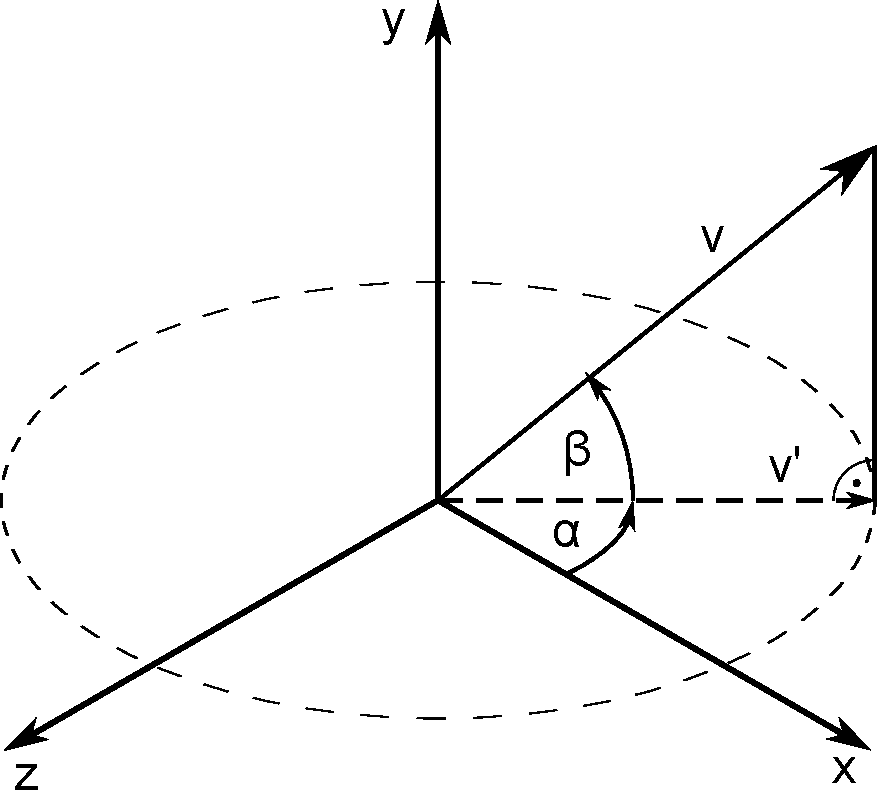
\includegraphics[width=10cm]{ilustrace/Il-9-1}
		\caption{Ilustrace rotace vektorem posunutí. $x$,$y$,$z$ - osy souřadného systému, v - vektor posunutí, $v'$ - kolmý průmět $v$ do roviny $XZ$, $\alpha$ - úhel označující velikost rotace v kolem osy Y, $\beta$ - úhel označující velikost odklonu v od roviny $XZ$, pro změnu směru vektoru bude k úhlu $\alpha$ přičtena hodnota úhlu $yaw$, kterou zadá uživatel, k úhlu $\beta$ bude přičtena hodnota úhlu $pitch$}
		\label{fig:9-1}
	\end{center}
\end{figure}

\subsection{Orientace scény}
Problém ovšem nastává v tom, jak určit vektor vzhůru.
\paragraph{}
Scéna získaná programem Bundler obsahuje kamery přibližně v rovine $XZ$ a kladná část osy $Y$ míří přibližně vzhůru. Scéna z programu VisualSFM má kamery také přibližně v rovině $XZ$, ale celá scéna je otočena kolem osy $X$ o $180^{\circ}$, takže pro scénu jsou osy $Y$ a $Z$ převráceny. Přesnou orientaci scény nejsme schopni získat z pozice ani z orientace kamer. I kdyby byly kamery přesně v jedné rovině, tak bychom stále nemohli říci, že tato rovina je rovnoběžná se zemí, neboť rekonstruovaný objekt mohl být focen ze svahu. 
\paragraph{}
Možností by bylo nechat uživatele, aby zadal vektor směřující vzhůru, ale to by uživateli zbytečně přidělávalo další starost, neboť by musel sám zadávat hodnoty vektoru.
\paragraph{}
Zvolím proto rovinu $XZ$ jako zemi a kladnou část osy $Y$ jako směr vzhůru. To znamená, že rotace ve scéně z programu VisualSFM budou prováděny na druhou stranu než ve scéně z programu Bundler, ale to by uživateli nemělo činit problém.

\subsection{Zadání úprav vektoru}
Bude třeba, aby uživatel zadal 3 hodnoty (velikost a 2 úhly). Kvůli přesnosti budou vyžadována desetinná čísla. 
\paragraph{}
Jednou z možností je použít textová pole, kam uživatel napíše hodnotu, která se má použít. Takto zadaný řetězec znaků se následně přeparsuje na hodnotu. Problém nastane, pokud uživatel zadá cokoliv jiného než desetinné číslo.
\paragraph{}
Další možností by bylo použít slider. Táhlo, kterým by uživatel nastavil konkrétní hodnotu. Tato možnost by umožnila rychlejší nastavení hodnot, ale s menší přesností. Problém této možnosti je v nezbytnosti rozsahu, v jakém může slider nabývat hodnot. V případě úhlů toto není problém, jelikož nabývají hodnot od $0^{\circ}$ do $360^{\circ}$, ale vzdálenost omezená není. U vzdálenosti by bylo třeba nastavit nějakou základní hodnotu a v případě, že by uživatel potřeboval větší rozsah (dojel by sliderem na maximální hodnotu) zvětšila by se maximální hodnota a slider by se aktualizoval na nový stav. Dalším problémem je velikost slideru. Čím větší bude, tím přesnější bude hodnota zadaná uživatelem, ale tím více místa v GUI zabere.
\paragraph{}
Obě tyto možnosti mají nějaká pro a proti. Každému uživateli může vyhovovat jiný nástroj. Proto použiji pro velikost vektoru textové pole a pro úhly jak textová pole, tak slidery. Tato varianta bude ovšem vyžadovat zvětšení okna editoru, aby se do něj vešla nová textová pole a slidery. Zároveň bude nezbytné synchronizovat textová pole pro úhly s jejich slidery, aby vždy ukazovali stejné hodnoty. 

\subsection{Uložení hodnot}
Každá plocha bude potřebovat vektor, 2 úhly a velikost výsledného vektoru, abychom mohli vytvořit trojrozměrné těleso. Tyto proměnné bude třeba přidat do třídy reprezentující plochy, tj. CSG\_Plane.
\paragraph{}
Také bude vhodné přidat proměnné pro úhly a vzdálenost do třídy editoru, tj. MDI\_editor\_v1. Díky tomu bude možné snadno synchronizovat vybranou plochu se stavem GUI. Zároveň nám toto dovolí návrat k poslední správné hodnotě, pokud uživatel zadá do textového pole nečíselnou hodnotu\footnote{Teoreticky by bylo možné použít data slideru pro uchování hodnoty úhlu, ale hodnoty slideru mohou být pouze celá čísla. I když určíme, že jedna jednotka na slideru odpovídá například $0.1^{\circ}$ otočení vektoru, nebude slider nabývat takového množství hodnot jako například datový typ float.}.

\subsection{Aktualizace GUI}
Také bude nezbytné provádět aktualizace hodnot v GUI editoru, pokud uživatel zvolí jinou plochu v paletě ploch. V tu chvíli je potřeba nastavit hodnoty obou úhlů i vzdálenost v editoru na hodnoty vybrané plochy. Pokud z plochy není vytvořeno trojrozměrné těleso, nastavily by se základní hodnoty, tj. velikost vektoru rovna jedné a úhly rovny nule. 

\subsection{Uložení geometrie trojrozměrného tělesa}
Místo geometrie jedné plochy teď bude potřeba vytvářet geometrii celého tělesa. Jak už jsem zmínil dríve (\ref{volbaMetody}), způsob vytváření geometrie je volen v metodě reconstructPlane třídy SegmentationWrapper. Odtud je volána konkrétní metoda vytvářející geometrii a její výsledek se ukládá do instance plochy.
\paragraph{}
Pokud tedy plocha má hranici tvořenou z n bodů, celé těleso bude mít n+2 stran. Pokud se tedy místo jednoho objektu GeometryArray vytvoří pole s $n+2$ objekty GeometryArray, bude možné využít stávající algoritmy pro vytváření 3D scény. Znamenalo by to tedy, že by byl třída CSG\_Plane měla kromě jedné proměnné typu GeometryArray uchovávající geometrii plochy ještě jedno pole typu GeometryArray[], které by uchovávalo druhou podstavu tělesa a boční stěny.

\subsection{Vytváření geometrie trojrozměrného tělesa}
Nyní potřebujeme vytvořit pole instancí GeometryArray, které reprezentuje trojrozměrné těleso. K tomu potřebujeme množinu 3D reprezentací bodů hranice dané plochy. Ty obstaráme obdobným způsobem, jako při ořezávání plochy pomocí hranice (viz. \ref{hraniceJedenBod}). Dále bude třeba znát vektor, který bude použit a úpravy, které na něj uživatel použit. To znamená 2 úhly\footnote{úhly $yaw$ a $pitch$} a délku vektoru.
\paragraph{}
Potřebujeme z původního vektoru vypočítat výsledný vektor. Nejprve se na vektor aplikuje rotace kolem obecné osy\footnote{Podrobnější informace o rotaci kolem obecné osy v Moderní počítačová grafika\cite{Zara}, část E, kapitola 21.3.3.} o úhel $pitch$. Tuto osu získáme vektorovým součinem mezi vektorem, který transformujeme a vektorem vzhůru, tj. osou $Y$. Tato rotace vlastně změní úhel mezi transformovaným vektorem a rovinou $XZ$.  Dále aplikujeme rotaci kolem osy $Y$ o úhel $yaw$ a výsledný vektor vynásobíme velikostí, kterou jsme získali od uživatele. Tímto jsme získali vektor posunutí.
\paragraph{}
Množinu trojrozměrných bodů, tj. průměrných bodů hranice, použijeme jako body první podstavy. Body druhé podstavy získáme z bodů první podstavy, ke kterým přičteme výše zmíněný vektor posunutí.
\paragraph{}
Pro vytváření jednotlivých instancí GeometryArray použijeme třídu GeometryInfo jako při vytváření plochy. Pro geometrii první podstavy použijeme neposunuté body. Pro geometrii druhé podstavy použijeme posunuté body. A pro boční stěny využijeme vždy dva po sobě jdoucí posunuté body a jim odpovídající neposunuté body (první a poslední bod jsou také brány jako po sobě jdoucí body). 

\subsection{Výpočet texturovacích souřadnic trojrozměrného tělesa}
Podle výsledku části \ref{teturovaniTelesa} bude trojrozměrné těleso texturováno tak, že trojrozměrné body tělesa budou promítnuty do fotografie a takto získané souřadnice budou převedeny na texturovací souřadnice jako v části \ref{texturovacíSouřadnice}. Takto získané texturovací souřadnice budou přidány ke geometriím při jejich vytváření.

\subsection{Zobrazení tělesa ve scéně}
Pro připojení geometrie plochy ke scéně slouží metoda createPlane třídy CSG3D. Tuto metodu bude třeba upravit tak, že kromě vytváření plochy zjistí, zda má být vytvořeno i trojrozměrné těleso z plochy. Pokud ano, vytvoří všechny zbylé stěny tohoto tělesa, připojí k nim materiál a vzhled, který je připojován k původní ploše a následně připojí tyto stěny ke scéně.


%
%
%
\chapter{Implementace}
V této části práce popíši implementaci vybraných tříd a metod, které byly navrhnuty v předchozích kapitolách (\ref{navrhStart} - \ref{navrhEnd}).

\section{Importní modul pro VisualSFM}
Do nabídky v hlavním okně programu jsem k Import Bundler přidal možnost Import VisualSFM. Dále jsem vytvořil metodu loadScene(String path) která jako parametr přijímá cestu k souboru s informacemi o kamerách a bodech ("bundle.out" nebo "bundle.rd.out") a její obsah je kopií obslužné metody pro načítáí dat z Bundleru. Nyní obsluha obou GUI elementů (Import bundler, Import VisualSFM) volá loadScene, ale každá s jiným parametrem. Tímto způsobem jsem se vyhnul duplicitám v kódu. 
\paragraph{}
V budoucnu tudíž může nastat problém, pokud by se změnil formát výstupních dat v jednom z těchto programů. V tom případě bude nutné obsluhu těchto elementů opět rozdělit.

\section{Nejvýznamnějsí změny v aplikaci}
Ze všech implementovaných věcí jsem vybral pouze ty části, které významně ovlivnily funkce, vnitřní struktury nebo vzhled programu. 

\subsection{Reprezentace hranice plochy}
Vytvořil jsem třídu PointBorder, která reprezentuje jeden bod hranice. Tento bod si uchovává informaci, ve kterých fotografiích byl zadán a na jakých pozicích byl zadán.  Také má informaci do které roviny bude promítán. Dále tato třída obsahuje metody pro promítání jednotlivých hraničních bodů i jejich kolekcí do roviny, nebo pro promítání trojrozměrných bodů do fotografií. Dalšími metodami jsou například metody pro výpočty texturovacích souřadnic, přidání dalších fotografií, ve kterých byl bod zadán a pozic, na kterých byl zadán, a také odstraňování těchto informací.
\paragraph{}
Při promítání je tento hraniční bod promítnut do roviny ze všech fotografií, ve kterých byl zadán. Výsledný trojrozměrný bod je získán jako těžiště promítnutých bodů. Při obráceném postupu, tj. při promítání bodu do fotografie, se použije trojrozměrný bod, který je následně promítnut do fotografie.

\subsection{Promítání bodů kamerou}
Také bylo nezbytné vytvořit novou metodu project2DPoint2 ve třídě PinholeCamera\footnote{Původní metoda project2DPoint neprováděla projekci tak, jak se dalo od metody s tímto názvem očekávat. Z důvodu, že je tato metoda používána v jiných třídách, rozhodl jsem se raději implementovat novou metodu místo upravování stávající metody.}. Tato metoda vytváří z 2D bodu přímku, kde přímka odpovídá promítacímu paprsku (\ref{modelKamery}).

\subsection{Vytváření geometrie ploch}
Ve třídě Plane3Dutil jsem k metodě findBestVisualization4 vytvořil další dvě metody planeWithBorder a planeWithBorderAndExtrusion. Metoda planeWithBorder slouží k vytvoření geometrie plochy oříznuté hranicí. Metoda planeWithBorderAndExtrusion slouží k vytvoření geometrií reprezentujících trojrozměrné těleso vytvořené z plochy. První z těchto metod pro svou funkci vyžaduje, aby byla ploše zadána hranice z alespoň 3 bodů. Druhá metoda navíc vyžaduje, aby měla plocha nastaveny hodnoty pro vytvoření vektoru posunutí(viz. \ref{vektorPosunu}).  
\paragraph{}
Z těchto tří metod je v metodě reconstructPlane třídy SegmentationWrapper vybíráno na základě dat, která uživatel zadal.

\subsection{Zobrazení ploch v 3D scéně}
Jelikož nyní plocha nemusí být tvořena pouze jednou geometrií, ale může z ní být vytvořeno trojrozměrné těleso, bylo nezbytné upravit metodu createPlane ve třídě CSG3D.  Nyní tato metoda, pokud bylo z plochy vytvořeno trojrozměrné těleso, vytváří všechny stěny tohoto tělesa a připojuje je ke grafu scény.

\subsection{Nástroje přidané do editoru}
Do editoru fotografie jsem vytvořil k existujícímu nástroji pro kreslení do fotografie také nástroje pro zadávání bodů hranice, upravování bodů hranice, texturování plochy a vytváření trojrozměrného tělesa z plochy.

\subsection{Změny v GUI editoru}
Kvůli přidání dalších nástrojů do editoru bylo nezbytné provést řadu změn v GUI editoru. Do horní lišty jsem přidal možnost změny používaného nástroje, tlačítko pro otexturování právě vybrané plochy a možnost zafixovat nebo uvolnit bod ve fotografii (\ref{{fixaceBodu}}). 
\paragraph{}
Dále jsem přidal postranní panel pro vytváření trojrozměrného tělesa. Tento panel obsahuje dva slidery a jim dvě odpovídající textové pole pro nastavení úhlů. Dále je zde textové pole pro nastavení velikosti vektoru posunutí, tlačítko pro vytvoření trojrozměrného tělesa a také tlačítko pro nastavení základu vektoru posunutí na aktuální normálu plochy, kterou upravujeme.  

\subsection{Otestování a úprava editoru}
Po otestování nástroje pro vytváření tělesa z plochy jsem ještě přidal k postrannímu panelu checkBox "auto-extrude". Pokud je checkBox zaškrtnut, při jakýchkoliv změnách provedených v komponentách postranního panelu jsou změny okamžitě aplikovány na trojrozměrné těleso vytvořené z plochy. Tuto změnu jsem provedl z důvodu, že pokud se uživatel snaží nastavit přesné úhly, ale nemá velmi dobrý odhad, bude potřebovat aplikovat tyto změny několikrát. Uživatel by musel při každé této změně stisknout tlačítko, ale to by ho značně zdržovalo \footnote{Pro každou změnu by musel uživatel změnit pozici kurzoru, stisknout tlačítko a znovu upravit hodnotu. Toto by mu spotřebovalo hodně času obyčejnými činnostmi.}.

\begin{figure}[h]
	\begin{center}
		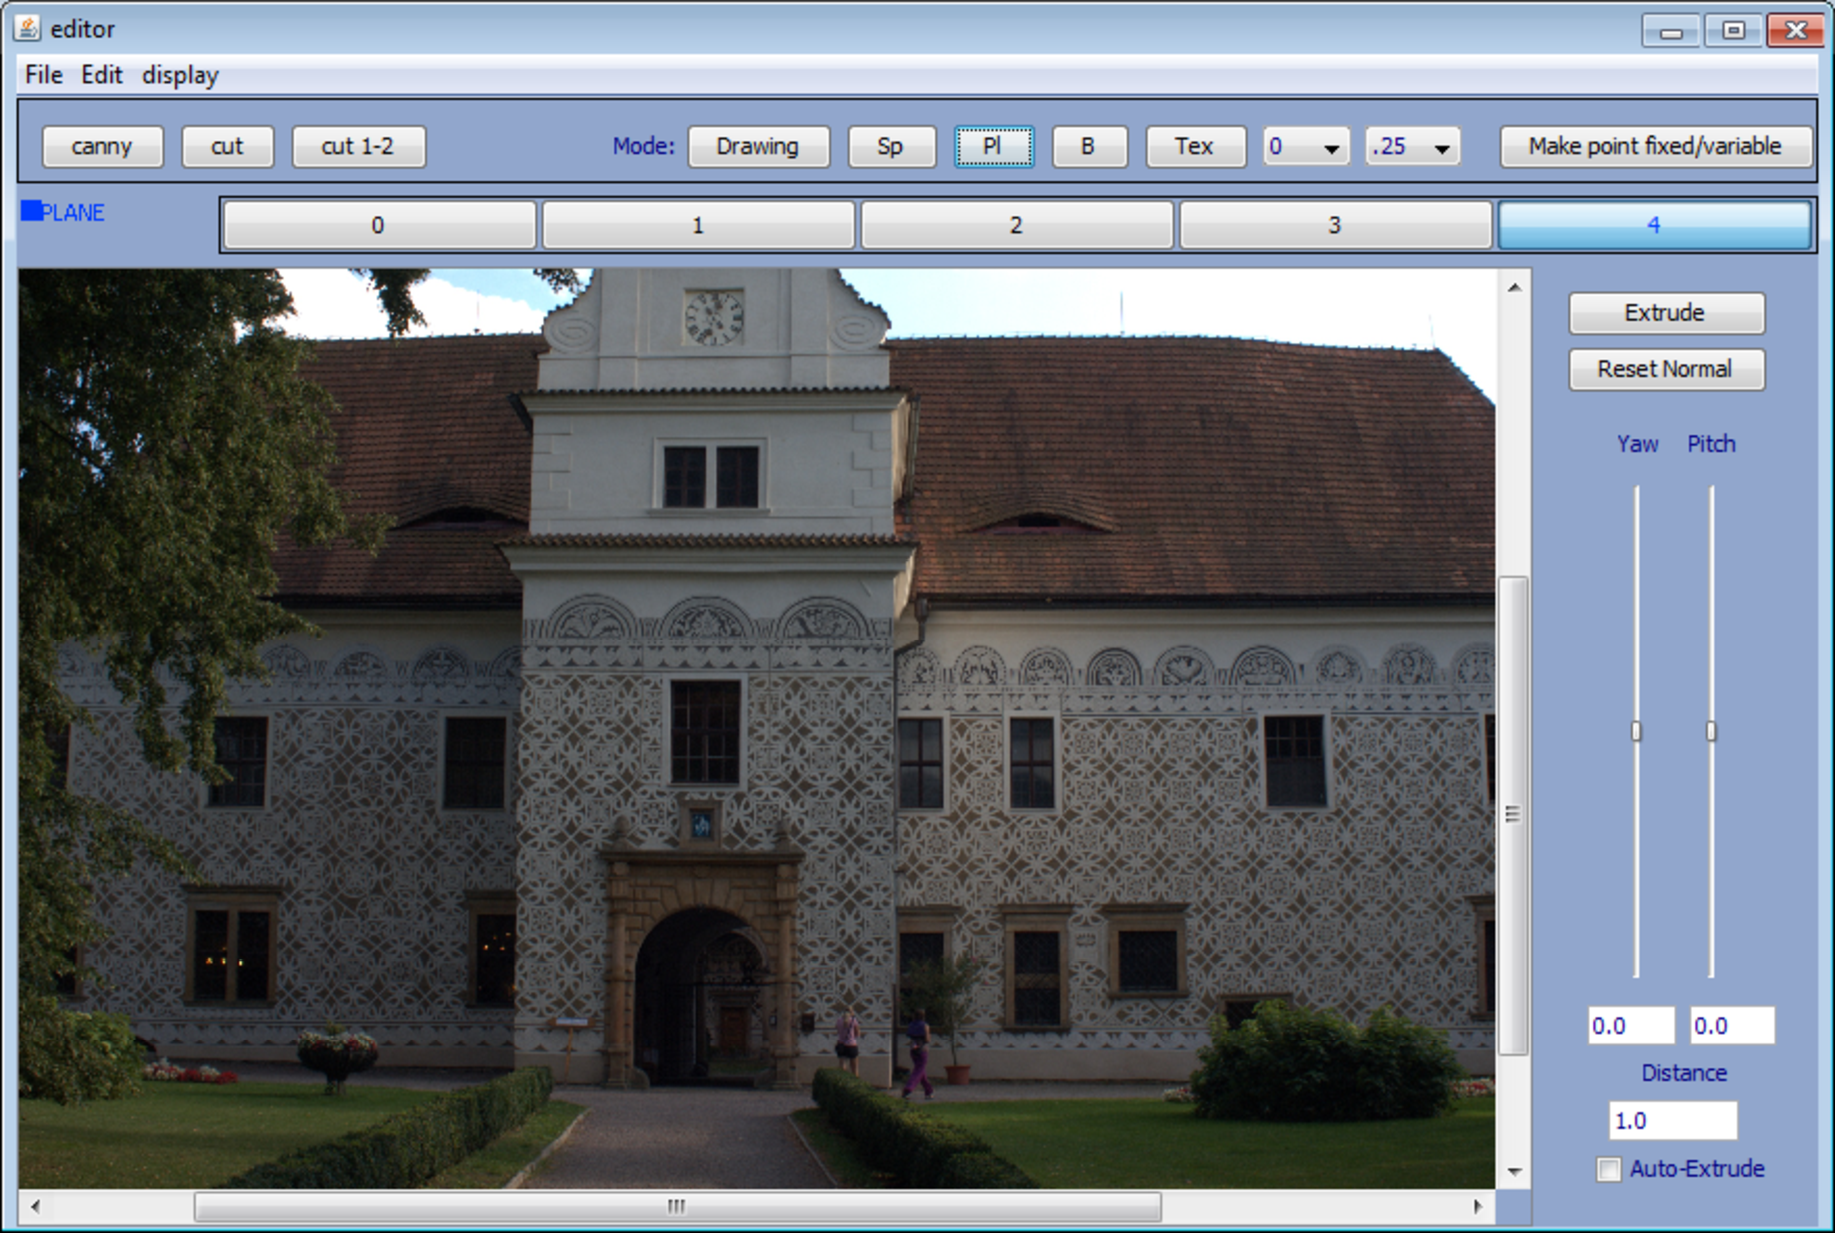
\includegraphics[width=10cm]{ilustrace/Il-5-1}
		\caption{Ilustrace znázorňující upravené okno editoru fotografie.}
		\label{fig:5-1}
	\end{center}
\end{figure}

\subsection{Otestování vytváření trojrozměrného tělesa plochy}
Po otestování nástroje pro vytváření trojrozměrných těles z plochy jsem se rozhodl k provedení drobné změny v GUI okna s 3D scénou. Do GUI jsem přidal checkBox označený jako" wireframe". Zároveň jsem provedl změnu v metodě, která vytváří vzhled objektu, jenž bude zobrazen ve scéně. Pokud je checkBox vybrán, všechny objekty (plochy i trojrozměrná tělesa) budou zobrazovány jako wireframe\footnote{Nejsou vykreslovány plochy, ale pouze hrany tělesa.}. K tomuto rozhodnutí mě vedl fakt, že jelikož ve scéně nejsou žádná světla a všechny objekty mají konstantní barvu, je poměrně obtížné od sebe rozeznat jednotlivé stěny tělesa a hrany mezi nimi, neboť mají konstantní barvy (v případě, že nejsou texturovány). Wireframe mód umožňuje uživateli lepší orientaci ve scéně a jednodušší nastavení vektoru posunutí pro vytváření trojrozměrného tělesa z plochy.

\section{Testování}
I když to nebylo v zadání mé práce, provedl jsem testy s uživateli. Toto testování jsem provedl se třemi uživateli a bylo nezbytné upravit podmínky testování. Upravení podmínek bylo nezbytné, neboť program je pouze experimentální. V GUI velmi často chybějí popisky tlačítek a některé nástroje z původní verze programu musely být uživatelům vysvětleny. Šlo především o testování, zda uživatel dokáže najít a správně použít nástroje přidané v rámci této práce. Dalším cílem testování bylo zjistit, jestli uživatelé budou schopni bez větších problémů nástroje používat, když už je vyzkoušeli a vědí, jak fungují. Zde šlo především o nástroj pro vytváření trojrozměrného tělesa z plochy a nástroje pro úpravy vektoru posunutí. Očekával jsem, že tato část by mohla být značný problém pro lidi se špatnou prostorovou představivostí\footnote{Proto jsem volil pro testování uživatele, kteří mají s prostorovou představivostí problém.}. 
\section{Výsledky testování}
V této kapitole popíši prolémy nalezené při testování a také návrhy, jak by bylo možné prolémy odstranit.

\subsection{1. nález - cyklický výběr nástrojů}
Prvním problémem, na který všichni tři uživatelé narazili bylo cyklické přepínání nástroji (\ref{cycle}). Pouze jediný z testujících uživatelů sám přišel na to, že je možné nástroje přepínat, ale jen proto, že zkoušel všechna tlačítka programu aby věděl, co dělají. Když už uživatelé o cyklickém přepínání věděli, dokázali tento výěr bez problémů použít.
\paragraph{}
Řešením problému by mohlo být přidání tlačítek, kde každému nástroji by odpovídalo jedno. Další řešení, stejně prostorově úsporné jako cyklický výběr, je použití "dropdown menu". Takto by uživatelé mohli snadno vybrat nástroj i v případě, že by jich v budoucnosti bylo větší množství. Zároveň většina uživatelů je zvyklá na klasické "dropdown menu"\footnote{Klasickým je myšleno běžné zobrazení, kde je vedle vybrané položky zobrazena šipka směřující dolů. }, což by je hned upozornilo na to, že zde mohou něco vybírat.

\subsection{2. nález - fotografie}
S tímto problémem se setkali všichni uživatelé, kteří program testovali. Když uživatel pracuje ve více fotografiích, především když zadává hranice ploch a následně je upravuje ve více fotografiích, pomalu začne ztrácet přehled o tom, ve které fotografii něco upravil. Problém značně zpomaluje uživatele při práci, když scéna obsahuje několik desítek fotografií a uživatel upravuje dříve zadané body. 
\paragraph{}
Efektivním řešením tohoto problému by bylo označování fotografií v Info panelu, pokud bylo do této fotografie něco přidáno, nebo v ní bylo něco upraveno. 

\subsection{3. nález - pohyb ve 3D scéně}
Uživatelé měli poměrně veliký problém s pohybem ve 3D scéně. Především problém s rotováním pohledové kamery kolem středu souřadné soustavy scény. Další problém byl v tom, že se uživatelům často otočila kamera podle její osy $Z$ a uživatelé nemohli přijít na to, jak kameru natočit zpět.
\paragraph{}
Tento problém by bylo snadné vyřešit tím, že by uživatelům bylo umožněno rotovat pohledovou kamerou vůči středu její souřadné soustavy.

\subsection{4. nález - nástroje v editoru}
Dva ze tří testujících uživatelů meli problém především s tím, že při jakémkoliv kliknutí do fotografie byla provedena nějaká činnost. I když se snažili pouze dostat okno s editorem do popředí. Zároveň se uživatelé snažili pohybovat s fotografií v editoru pomocí myši místo pomocí "scroll barů".
\paragraph{}
Toto by bylo možné vyřešit přidáním neutrálního nástroje, který nebude dělat nic při kliknutí do fotografie, nebo ještě lépe přidáním nástroje, který dovolí posun fotografie myší. 

\subsection{Menší problémy}
Černé označení vybraného bodu může být trochu matoucí pro některé uživatele. Dva z testujících uživatelů si mysleli, že vybraný bod byl odstraněn. Dále u vybraného bodu není poznat, zda je zadán ve zobrazené fotografii, nebo zda je do ní pouze promítán, když není vidět okraj bodu.
\paragraph{}
Uživatelé se snažili fotografii v editoru zvětšovat a změnšovat pomocí kolečka myši. To pouze způsobovalo posun fotografie v editoru.
\paragraph{}
Nástroj pro zvětšování a změnšování fotografie má na výběr pouze velmi omezené množství hodnot. To bránilo především při zmenšování fotografie k nastavení požadované velikosti\footnote{Pro hodnotu zvětšení 0.25 byla fotografie ještě příliš veliká, ale pro hodnotu 0.1 byla fotografie už příliš malá.}. Toto by bylo možné vyřešit zvětšováním a změnšováním fotografie pomocí otáčení kolečka myši, kde by se procházelo větší množství hodnot.

\subsection{Záver testování}
Všechny výše zmíněné nálezy by bylo vhodné v budoucnu odstranit, ale žádný z nich není tak vážný, že by bránil v použití aplikace.
\paragraph{}
Hlavní problém, který se vyskytl, byl ten, že uživatelé testující program měli problém spojit si správný nástroj s činností, kterou měli vykonat. To bylo výrazně ovlivněno tím, že uživatelé nebyli obeznámeni s pojmy jako například "textura" nebo "extrude". Také úroveň angličtiny některých testujících uživatelů nebyla příliš vysoká. Takže není možné říci, že tento problém byl způsobe pouze programem, ale bylo by vhodné se na něj v budoucnu více zaměřit a podle toho upravit GUI. Především nástroje pro rotaci a zvětšení/změnšení fotografie nejsou popsány vůbec a nástroj pro přidání dalších ploch je popsán "Pl" což uživateli, který s programem dřív nepracoval, nic neřekne.
\paragraph{}
Během testování bylo také zjištěno, že když uživatelé přišli na to, jak používat nástroj pro vytváření 3D tělesa z plochy a nástroj pro úpravu vektoru posunutí, už jim nedělalo prakticky žádný problém s jeho použitím\footnote{Když uživatelé přišli na analogii mezi rotací vektorem a pohybem hlavy (viz. \ref{rotace}), dokázali upravit směr vektoru ve velmi krátkém čase bez jediného problému.}.  

%
%
%
\chapter{Závěr}
Program předtím umožňoval uživateli prokládání množin bodů plochami a ořezávání ploch mezi sebou. Toto bylo vhodné pro poměrně jednoduché modely budov. Nyní uživatel může vytvářet stěny s poměrně složitými tvary, které budou přesně odpovídat jeho přáním. Dále může na tyto stěny aplikovat texturu z libovolné fotografie, kterou má k dispozici ve scéně. Navíc je uživatel schopen vytvářet trojrozměrné objekty k reprezentaci složitějších tvarů jako jsou římsy, sloupy nebo střechy. S těmito nástroji už je uživatel schopen vytvářet poměrně složité objekty a budovy v krátkém čase. Všechny nástroje, které byly do programu přidány jsou poměrně efektivní, když uživatel ví, jak nástroje fungují a jak s nimi pracovat. Zároveň množství přidaných nástrojů není veliké, takže by nemělo dojít k tomu, že by se uživatel v aplikaci ztrácel.

\clearpage

\begin{figure}[]
	\begin{center}
		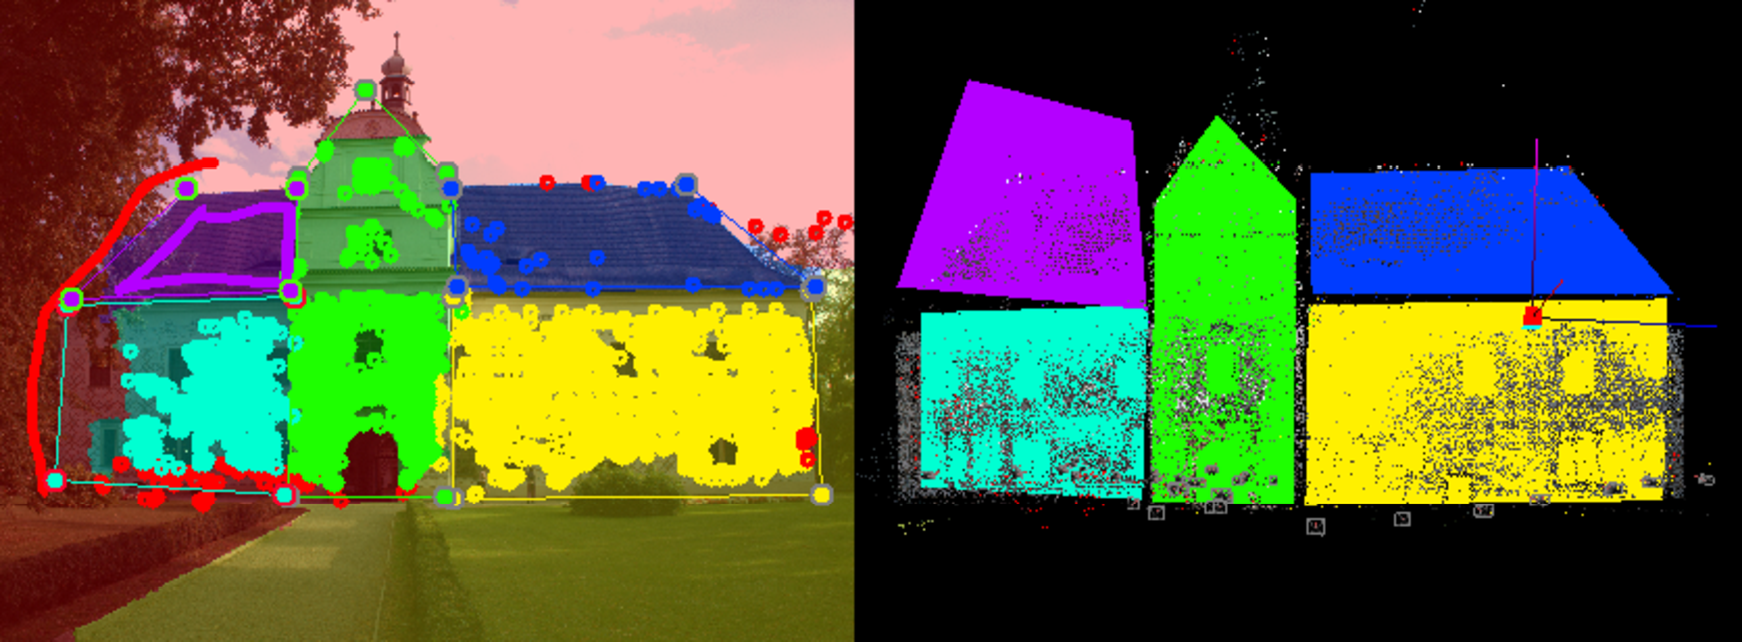
\includegraphics[width=15cm]{ilustrace/program/P-4}
		\caption{Ilustrace ploch s aplikovanými hranicemi. Vlevo je možné vidět fotografii s daty pro vytvoření ploch a hranicemi zadanými pro jednotlivé plochy. Vpravo je vidět 3D scénu s plochami oříznutými podle hranic.}
		\label{fig:P-4}
	\end{center}
\end{figure}

\begin{figure}[]
	\begin{center}
		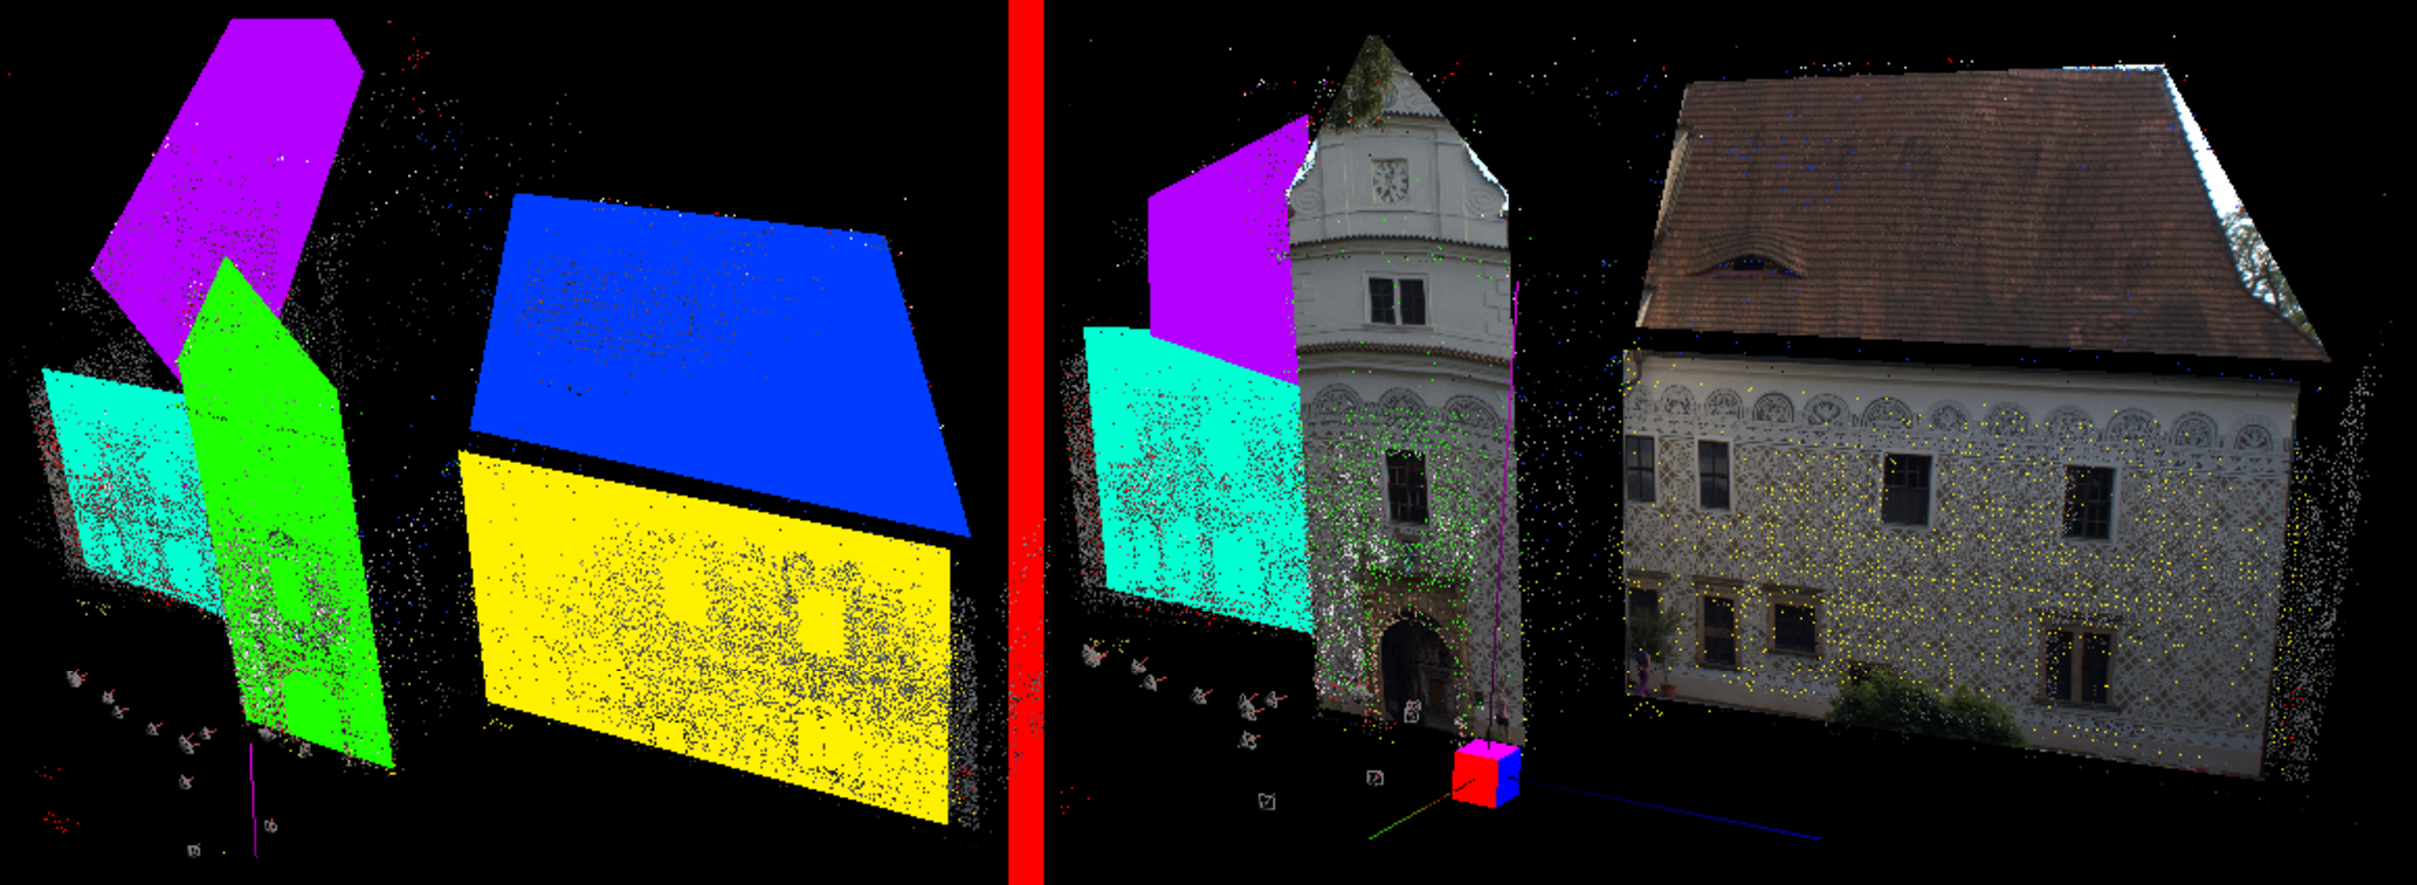
\includegraphics[width=15cm]{ilustrace/program/P-5}
		\caption{Ilustrace otexturovaných ploch. Vlevo je možné vidět 3D scénu před aplikováním textury a vpravo je na tmavěmodrou, žlutou a zelenou oříznutou plochu aplikována textura z jedné z fotografií. Oříznuté plochy jsou schodné s plochami z obrázku \ref{fig:P-4}), jen každá svéna je zobrazena z jiného úhlu.(Zde je dobře vidět jak fialová plocha má pokaždé jiný sklon, to je způsobeno tím, že byly ploše přiřazeny i body, které by do ní patřit neměly. Plocha se poté s každým novým vygenerováním značně změní.)}
		\label{fig:P-5}
	\end{center}
\end{figure}

\begin{figure}[]
	\begin{center}
		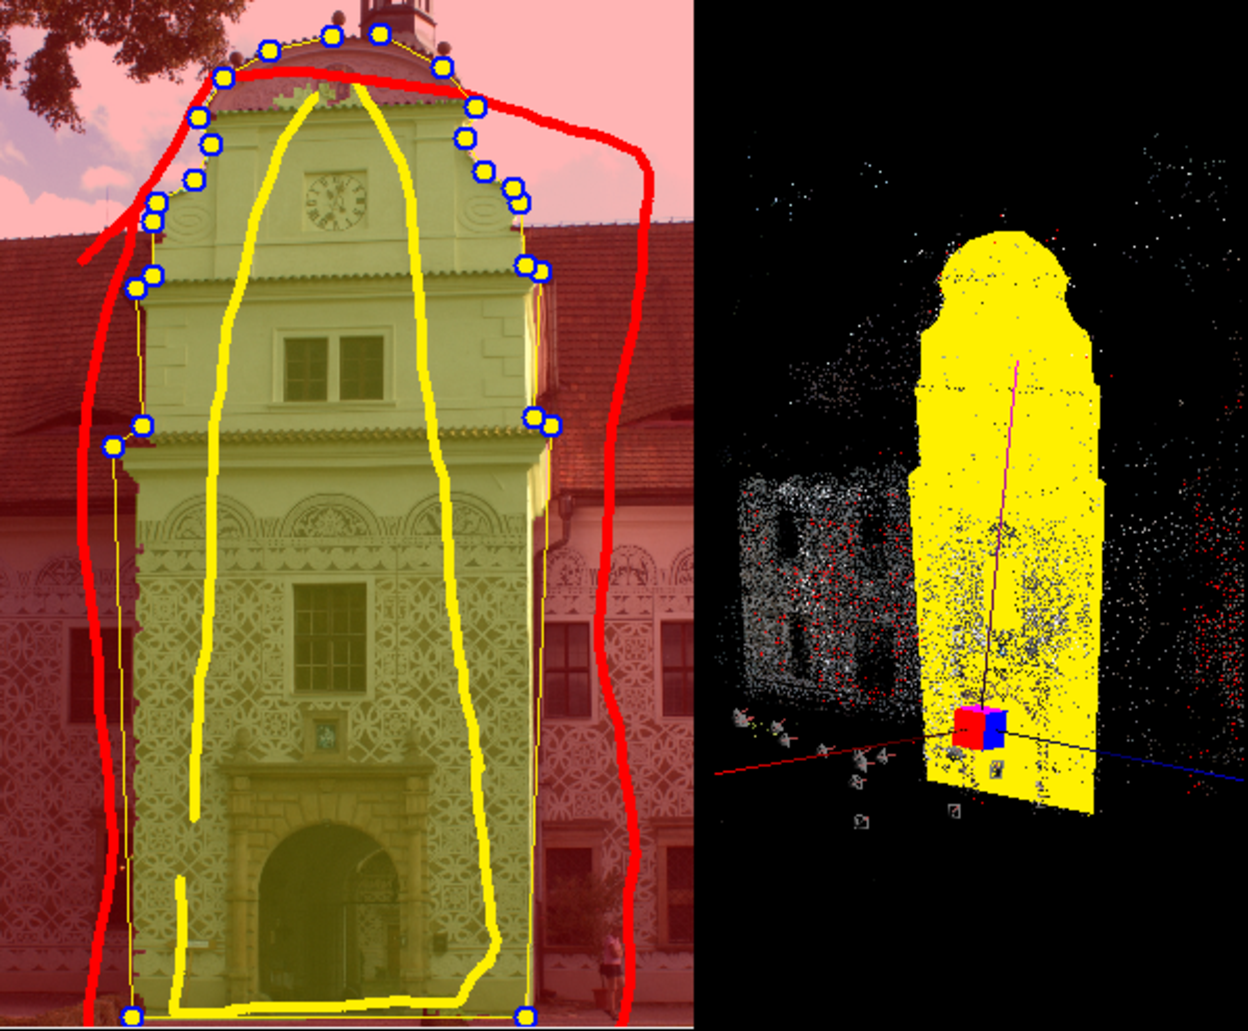
\includegraphics[width=15cm]{ilustrace/program/P-6}
		\caption{Ilustrace použití složitější hranice. Vlevo je fotografie v editoru s hranicí. Vpravo je plocha s aplikovanou hranicí ve 3D scéně.}
		\label{fig:P-6}
	\end{center}
\end{figure}

\begin{figure}[]
	\begin{center}
		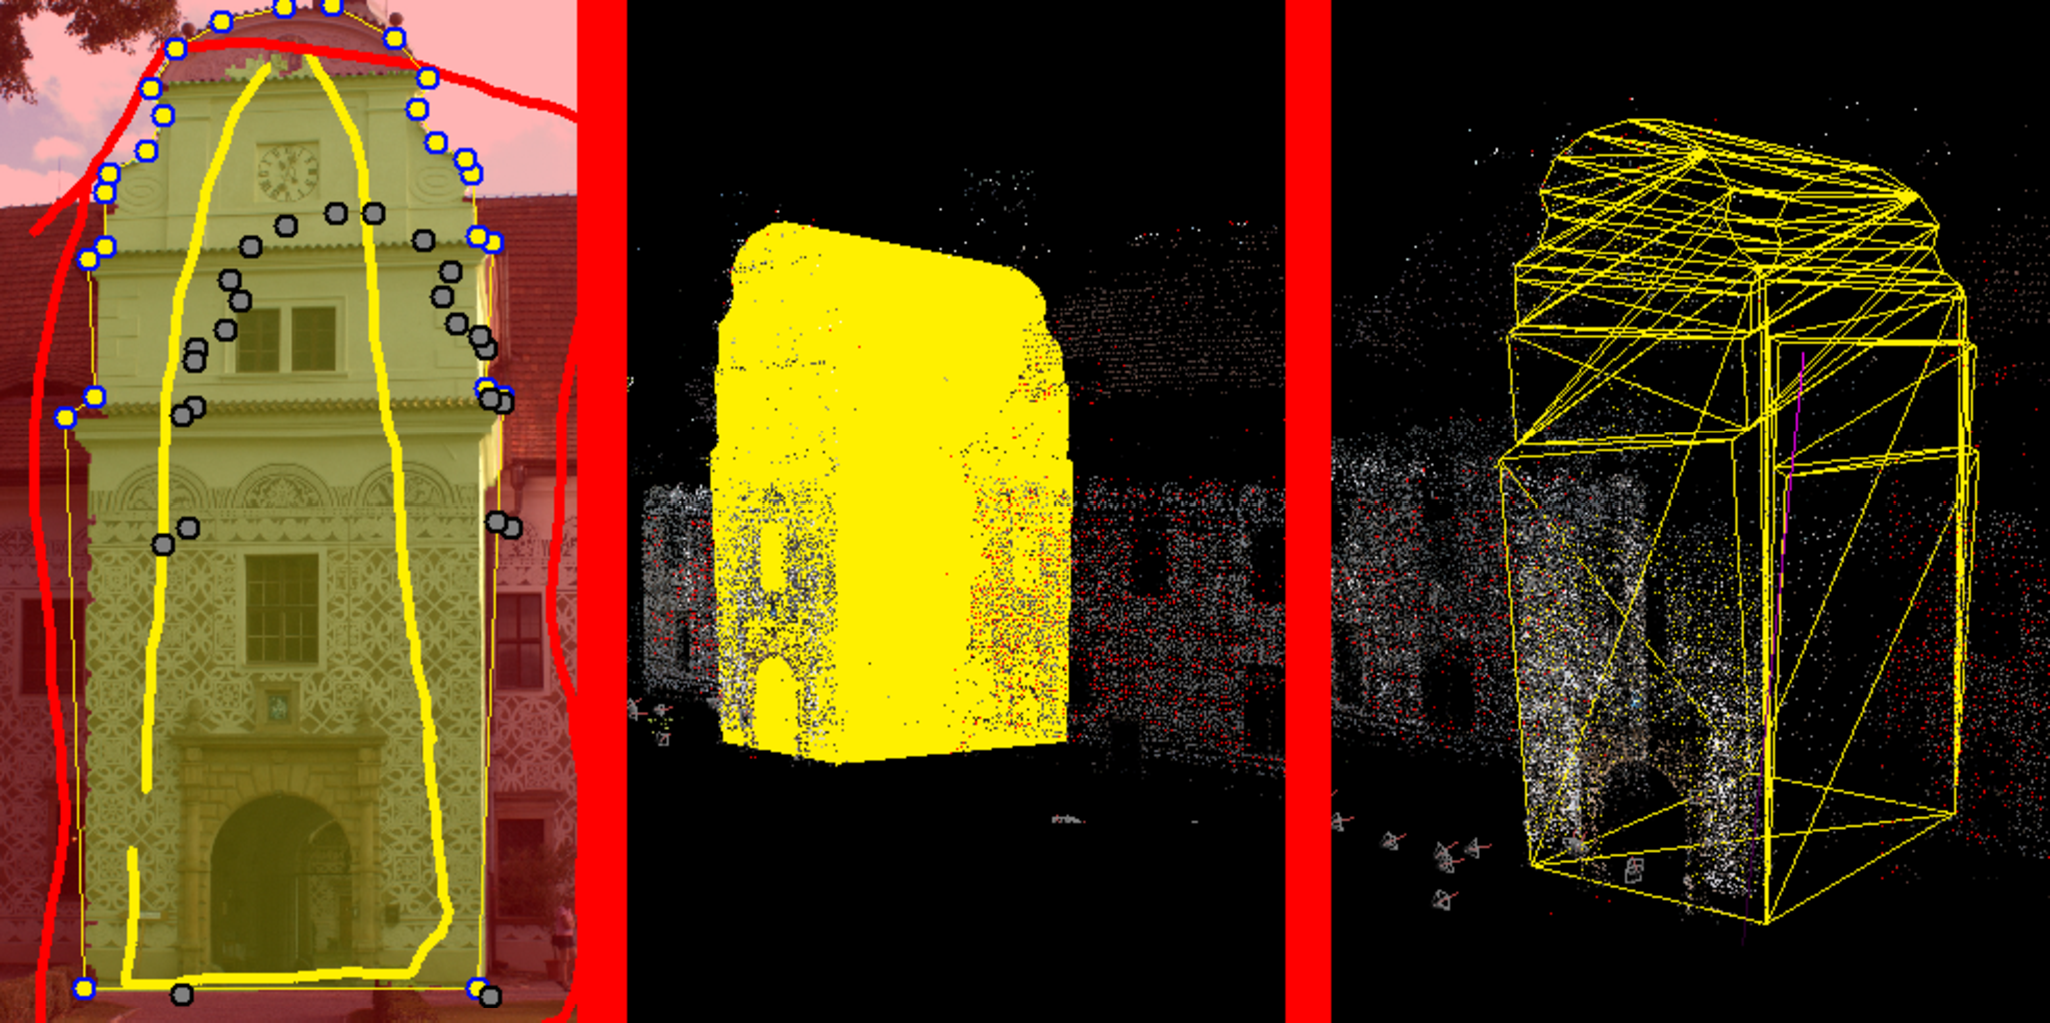
\includegraphics[width=15cm]{ilustrace/program/P-7}
		\caption{Ilustrace vytváření 3D tělesa. Vlevo je fotografie ve zadanou žlutou plochou a hranicí, ze které bylo vytvořeno 3D těleso.(Šedé body s černým okrajem jsou body 2. podstavy tělesa promítnuté do fotografie.) Uprostřed je těleso ve 3D scéně v normálním módu zobrazení. Vpravo je stejné těleso ve 3D scéně zobrazené ve wireframe módu. }
		\label{fig:P-7}
	\end{center}
\end{figure}


\bibliographystyle{csplainnat}

%bibliographystyle{plain}
%\bibliographystyle{psc}
{
\def\CS{$\cal C\kern-0.1667em\lower.5ex\hbox{$\cal S$}\kern-0.075em $}
\bibliography{lit}
}


\appendix	
\printnomenclature
\chapter{Obsah přiloženého DVD}
DVD přiložené k práci obsahuje především text této práce ve zdrojovém formátu (\LaTeX), tak i ve formátu PDF. Kromě toho také obsahuje projekt s upravenou aplikací ArchiRec3D s dokumentací\footnote{Původní aplikace neměla žádnou dokumentaci, proto dokumentace obsahuje pouze popis tříd a metod, které byly vytvořeny/upraveny v průběhu této práce.} a dalšími soubory. Podrobnější informace jsou k nalezení v souboru README.txt na přiloženém DVD.

\vspace{8mm}
Obsah:
\vspace{3mm}

$\backslash text$ \hspace{15mm} Adresář s textem práce ve zdrojovém formátu a v pdf.

$\backslash project$	\hspace{10mm} Adresář obsahující projekt, dokumentaci, testovací data a další.

$\backslash README.txt$	\hspace{10mm} Soubor obsahuje detailní popis obsahu DVD.

\end{document}